% ******************************************************** %
% DOCUMENT INFORMATION                                     %
% ******************************************************** %
%                                                          %
%                                                          %
% Purpose of Document                                      %
% -------------------                                      %
% Technical Report                                         %
%                                                          %
% Institution                                              %
% -----------                                              %
% University of Applied Sciences and Arts Northwestern     %
% Switzerland, School of Engineering                       %
%                                                          %
% Degree Program                                           %
% --------------                                           %
% Electrical Engineering and Information Technology, BSc.  %
%                                                          %
% Course                                                   %
% ------                                                   %
% Project 5, Fall Semester 2016                            %
%                                                          %
% Authors                                                  %
% -------                                                  %
% Raphael Frey                                             %
% Alex Murray                                              %
%                                                          %
% Document Design and Maintenance                          %
% -------------------------------                          %
% Raphael Frey                                             %
% Based on my own work. The  template on which this report %
% was based is available at:                               %
% https://github.com/alpenwasser/longtex                   %
% -------------------------------------------------------- %

\documentclass[11pt, a4paper, oneside]{memoir}

% -------------------------------------------------------- %
% Different font and pages  sizes, layouts. Not a complete %
% list, just what I've used on occasion.                   %
% -------------------------------------------------------- %
%\documentclass[9pt,b5paper]{memoir}
%\documentclass[twocolumn,9pt,a4paper]{memoir}
%\documentclass[10pt,a5paper]{memoir} % ~60 chars per line
%\documentclass[12pt,a4paper]{memoir} % ~60 to 70 chars per line


% -------------------------------------------------------- %
% Preamble  stuff  is  kept in  the  preamble/  directory, %
% separated  out into  different files  as needed  to keep %
% things modular.                                          %
% -------------------------------------------------------- %
% -------------------------------------------------------- %
% NOTE: There   are  two   kinds  of   packages  in   this %
% document. On ond hand, there  are those which are needed %
% for this  template to function at  as intended. It might %
% still  compile without  them,  but it  will probably  no %
% longer look as it should.                                %
%                                                          %
% On the other hand, there are those which I have found to %
% be useful over the years  and tend to commonly use.  You %
% may or may  not need those.  Feel free  to disable those %
% you do not need.                                         %
%                                                          %
% By default,  I recommend leaving the  following packages %
% enabled:                                                 %
% - fontenc: for output font encoding                      %
% - inputenc: for using  non-standard characters in input, %
%   such as Umlauts or other accented characters           %
% - graphicx:  needed for  the  chapter  style (based  on  %
%   veelo)                                                 %
%                                                          %
% Feel free to  disable and enable the  rest as needed. If %
% the document no longer compiles or breaks aesthetically, %
% you will notice soon enough...                           %
% -------------------------------------------------------- %


% -------------------------------------------------------- %
% General Packages                                         %
% -------------------------------------------------------- %
\usepackage[T1]{fontenc}     % output encoding
\usepackage[utf8]{inputenc}  % input encoding
\usepackage[english]{babel}
\usepackage{lipsum}          % filler text

% -------------------------------------------------------- %
% xcolor  and kvoptions  are  loaded by  xcolor-solarized. %
% If   you  require   special   options   for  these   two %
% packages,  uncomment  these  two lines  and  pass  those %
% options. Otherwise  leave them  commented out  since the %
% packages are loaded anyway.                              %
% We load xcolor here to avoid a package option conflict   %
% -------------------------------------------------------- %
\usepackage[table]{xcolor}
%\usepackage{kvoptions}
%\usepackage[prefix=sol]{xcolor-solarized}
\usepackage{xcolor-solarized}

% -------------------------------------------------------- %
% General Packages, continued                              %
% -------------------------------------------------------- %
\usepackage{graphicx}
\usepackage{amsmath}         % for reasonable math typesetting
\usepackage{pdfpages}        % include pdf documents
\usepackage{adjustbox}       % helps w/ minipage alignmant
\usepackage{pbox}            % boxes w/ line breaks in tables
\usepackage[textsize=footnotesize, textwidth = 37mm, english, colorinlistoftodos]{todonotes}
\usepackage{calc}            % used for calculating margins and widths for A3 pages
\usepackage[separate-uncertainty=true]{siunitx}
\usepackage[light]{kpfonts}
\usepackage{counttexruns}
\usepackage[european,siunitx,cuteinductors]{circuitikz}
\usepackage{adjustbox}
\usepackage{microtype}
%\usepackage{amsfonts}        % not sure yet if we need this
%\usepackage{caption}         % captions outside float environments, overrides memoir's caption facilities
%\usepackage{subcaption} % same as the caption package, seems to override memoir's own caption configs
%\usepackage{datetime2}
\usepackage{wrapfig}
\usepackage{listings}
%\usepackage{titletoc}        % TOC per chapter

%\overfullrule=2cm


% -------------------------------------------------------- %
% Draft Watermark                                          %
%                                                          %
% Prints  a watermark  across the  page, marking  it as  a %
% draft.                                                   %
% -------------------------------------------------------- %
%\usepackage{draftwatermark}
%\SetWatermarkText{Entwurf, \today}
%\SetWatermarkScale{0.5}
%\usepackage[final]{draftwatermark} % removes watermark


% -------------------------------------------------------- %
% TIKZ and PGF                                             %
%                                                          %
% TODO: See if this  should be put in a  separate file, or %
% if  having  it  here makes  sense. Alternatively,  these %
% documents might not need to be set globally at all.      %
% -------------------------------------------------------- %
\usepackage{tikz}
\usetikzlibrary{arrows}
\usetikzlibrary{graphs}
\usetikzlibrary{spy}
\usetikzlibrary{fit}
\usetikzlibrary{backgrounds}
\usetikzlibrary{positioning}
\usetikzlibrary{shapes.misc}
\usetikzlibrary{shapes.geometric}
\usetikzlibrary{shapes.symbols}
\usetikzlibrary{decorations.pathmorphing}
\usepackage{pgfplots}
\usepackage{pgfplotstable}
%\usepgfplotslibrary{units}
\usetikzlibrary{pgfplots.units}
\pgfplotsset{compat=1.10}
\pgfplotsset{max space between ticks=80pt}
\pgfplotsset{max space between ticks=80pt}
\pgfplotsset{try min ticks=5}
\pgfplotsset{
    tick label style={font=\small},
    label style={font=\small},
    legend style={font=\footnotesize}
}
\pgfplotsset{every axis plot/.append style={%
    line width=0.5pt}}
\usepgfplotslibrary{colormaps}
\usepgfplotslibrary{external}
\tikzexternalize[prefix=cache/]

\usepackage{bytefield}


% -------------------------------------------------------- %
% Conditionals                                             %
% -------------------------------------------------------- %
% http://tex.stackexchange.com/questions/5894/latex-conditional-expression
\usepackage{etoolbox}

% -------------------------------------------------------- %
% Packages which might be used under certain circumstances %
% -------------------------------------------------------- %
%\usepackage{geometry}
%\usepackage[english]{babel}
%\usepackage{kpfonts}

% -------------------------------------------------------- %
% Set link  colors and  all that good  stuff. See hyperref %
% manual for more info and options if you wish.            %
% -------------------------------------------------------- %
\newtoggle{paper}
%\toggletrue{paper} % we're printing on paper
\togglefalse{paper} % we're making an electronic version

\iftoggle{paper}{%
    % ---------------------------------------------------- %
    % If  we're  printing on  paper,  don't  do any  fancy %
    % coloring for links and such.                         %
    % ---------------------------------------------------- %
    \usepackage[%
        bookmarksnumbered=true,
        colorlinks=true,
        linkcolor=black,
        citecolor=black,
        urlcolor=black,
        %hidelinks=false,
    ]{hyperref}
}{%
    % ---------------------------------------------------- %
    % If  we're  creating  an electronic  version  of  our %
    % document, color links as follows.                    %
    % ---------------------------------------------------- %
    \usepackage[%
        bookmarksnumbered=true,
        colorlinks=true,
        linkcolor=blue,
        citecolor=solarized-cyan,
        urlcolor=purple,
        %hidelinks=false,
    ]{hyperref}
}

% -------------------------------------------------------- %
% Input Listing Formatting                                 %
% -------------------------------------------------------- %
\lstdefinestyle{txt}{
    aboveskip           = 3mm,
    belowskip           = 3mm,
    showstringspaces    = false,
    columns             = flexible,
    keepspaces          = true,
    basicstyle          = {\scriptsize\ttfamily},
    numbers             = left,
    numberstyle         = \tiny\color{gray},
    breaklines          = true,
    breakatwhitespace   = true,
    tabsize             = 3
}

% -------------------------------------------------------- %
% This file contains various options for the memoir class  %
% itself.                                                  %
% -------------------------------------------------------- %


% -------------------------------------------------------- %
% Rename Appendices to whatever we want.                   %
% See p78 of memman.pdf                                    %
% -------------------------------------------------------- %
%\def\appendixpagename{\sffamily\HUGE Anh\"ange}
%\def\appendixtocname{Anh\"ange}

% -------------------------------------------------------- %
% Choose a page layout                                     %
% -------------------------------------------------------- %
%                                                          %
% The  layout  is based  on isopage,  with  the  following %
% changes:                                                 %
% - The spine margin is 30 mm. This is so that binding the %
% document with  a ringbinder does  not come too  close to %
% the text.                                                %
% - The edge  margin is  1.5 times the spine  margin, i.e. %
% 45 mm.                                                   %
% - The top margin is 1/9  of the paper height, same as in %
% \isopage                                                 %
% - The bottom margin is decreased from isopage's value to %
% 1.5 times the top margin, i.e. about 50 mm.              %
% -------------------------------------------------------- %

%    +----------^--------------------+
%    |          | 33mm               |
%    |     +----v------------+       |
%    |30mm |                 | 45mm  |
%    |<--->|                 |<----->|
%    |     |                 |       |
%    |     |                 |       |
%    |     |                 |       |
%    |     |                 |       |
%    |     |                 |       |
%    |     |                 |       |
%    |     |                 |       |
%    |     |                 |       |
%    |     |                 |       |
%    |     |                 |       |
%    |     |                 |       |
%    |     |                 |       |
%    |     +----^------------+       |
%    |          | 49.5mm             |
%    |          |                    |
%    +----------v--------------------+
\isopage%
\setlrmarginsandblock{0.142857111\paperwidth}{0.190476190\paperwidth}{*}
\setulmarginsandblock{0.111111111\paperheight}{*}{1.5}%
\checkandfixthelayout%


% -------------------------------------------------------- %
% Choose a chapter style                                   %
% We're  going  with  veelo, but  removing  the  "Chapter" %
% designation in front of the chapter number.              %
% -------------------------------------------------------- %
% -------------------------------------------------------- %
% This  chapterstyle is  baesd on  veelo, but  removes the %
% "Chapter" designation in front of the chapter number.    %
% -------------------------------------------------------- %
%
% TODO: Check if this is allowed by the  LPPL, under which
% 'memoir.cls' is distributed, which contains the original
% code for the veelo chapter style.
%
% http://www.latex-project.org/lppl.txt
%
% If this is not permitted, implement alternative via this:
% http://tex.stackexchange.com/questions/51527/chapter-heading-with-the-word-chapter-replaced-by-chapter-name

\makeatletter
\makechapterstyle{fhnw}{%
    \setlength{\afterchapskip}{40pt}
    \renewcommand*{\chapterheadstart}{\vspace*{40pt}}
    \renewcommand*{\afterchapternum}{\par\nobreak\vskip 25pt}
    \renewcommand*{\chapnamefont}{\sffamily\LARGE\flushright}
    \renewcommand*{\chapnumfont}{\sffamily\HUGE}
    \renewcommand*{\chaptitlefont}{\sffamily\HUGE\bfseries\flushright}
    \renewcommand*{\printchaptername}{%
        \chapnamefont\MakeTextUppercase{}}
    \renewcommand*{\chapternamenum}{}
    \setlength{\beforechapskip}{18mm}%  \numberheight
    \setlength{\midchapskip}{\paperwidth}% \barlength
    \addtolength{\midchapskip}{-\textwidth}
    \addtolength{\midchapskip}{-\spinemargin}
    \renewcommand*{\printchapternum}{%
        \makebox[0pt][l]{%
            \hspace{.8em}%
            \resizebox{!}{\beforechapskip}{\chapnumfont \thechapter}%
            \hspace{.8em}%
            \rule{\midchapskip}{\beforechapskip}%
        }%
    }%
   \makeoddfoot{plain}{}{}{\thepage}%
}
\makeatother

\chapterstyle{fhnw} % requires graphicx package

\setsecheadstyle{\Large\bfseries\sffamily}
\setsubsecheadstyle{\large\bfseries\sffamily}
\setsubsubsecheadstyle{\bfseries\sffamily}

% -------------------------------------------------------- %
% Pagestyle (Headers, Footers)                             %
% -------------------------------------------------------- %
\pagestyle{headings}

% -------------------------------------------------------- %
% Cross Referencing Stuff                                  %
% -------------------------------------------------------- %

% Apparently these are not automatically translated into
% German by babel:
\def\figurerefname{Abbildung}
\def\tablerefname{Tabelle}
\def\pagerefname{Seite}

% -------------------------------------------------------- %
% Caption Configurations                                   %
% -------------------------------------------------------- %
\captionnamefont{\bfseries\small}
\captiontitlefont{\small}
\captiondelim{: }

% Captions for use outside of floats
\newfixedcaption{\figcaption}{figure}
\newfixedcaption{\tabcaption}{table}

% -------------------------------------------------------- %
% Define  what  sort  of  sectional  divisions  should  be %
% numbered.  See also "Document Divisions -- Numbering" in %
% the memoir manual.                                       %
%                                                          %
%            Division            |  Level                  %
%          ----------------------+---------                %
%            \book               |  -2                     %
%            \part               |  -1                     %
%            \chapter            |   0                     %
%            \section            |   1                     %
%            \subsection         |   2                     %
%            \subsubsection      |   3                     %
%            \paragraph          |   4                     %
%            \subparagraph       |   5                     %
%                                                          %
% \setsecnumdepth{<division>} sets  division numberings so %
% that <division>  and above will be  numbered.  When used %
% in  the preamble  (such as  here), \setsecnumdepth  also %
% calls \maxsecnumdepth, which is the numbering level used %
% in the \mainmatter part of the document. \setsecnumdepth %
% can be used anywhere  in the mainmatter to (temporarily) %
% change the numbering level.                              %
%                                                          %
% This template  uses chapters, sections,  subsections and %
% subsubsections  by default,  so  we  will set  numbering %
% level to subsubsection per default. Adjust as needed. We %
% will set this to subsubsection per default.              %
% -------------------------------------------------------- %
\setsecnumdepth{subsubsection}
\maxsecnumdepth{subsubsection}
\settocdepth{subsubsection}
\maxtocdepth{subsubsection}

\def\code#1{\texttt{#1}}
\def\quelleVA{\emph{Quelle:} Versuchsanleitung}
\def\anweisung{\emph{Anmerkung f\"ur Autoren: }}
\def\Raspi{Raspberry Pi}
\def\ISC{I\textsuperscript{2}C}


\definecolor{darkred}{rgb}{0.7,0,0}
\definecolor{darkblue}{rgb}{0.6,0.6,1}
\definecolor{darkgray}{gray}{0.4}
% checkmark
\newcommand{\checkmark}{\tikz\fill[fill=black!30!green,scale=0.4](0,.35) -- (.25,0) -- (1,.7) -- (.25,.15) -- cycle;}
% partially fulfilled
\newcommand{\partially}{\tikz\fill[fill=darkblue,scale=0.4](.5,0) -- (.55,.28) -- (.8,.33) -- (.55,.38) -- (.55,.62) -- (.8,.67) -- (.55,.72) -- (.5,1) -- (.45,.72) -- (.2,.67) -- (.45,.62) -- (.45,.38) -- (.2,.33) -- (.45,.28) -- cycle;}
% no indication
\newcommand{\noi}{\textcolor{darkgray}{\small\textsf{---}}}
% not present
\newcommand{\np}{\tikz\fill[fill=darkred,scale=0.4](0,0) -- (.5,.4) -- (1,0) -- (.6,.5) -- (1,1) -- (.5,.6) -- (0,1) -- (.4,.5) -- cycle;}
%\newcommand{\nv}{\textcolor{darkred}{$×$}}

\newcommand{\Sensor}{Sensor}
\newcommand{\Master}{Master-Ger\"at}

\newcommand{\myfancybreaksymbol}{\Diamond}
\newcommand{\myfancybreak}{\fancybreak{$\myfancybreaksymbol\quad\myfancybreaksymbol\quad\myfancybreaksymbol$}}

\newlength{\parindentbak}

\newcommand{\colorbitbox}[4]{%
    \rlap{\bitbox{#3}{\color{#1}\rule{\width}{\height}}}%
    \bitbox{#3}{\sffamily\textcolor{#2}{#4}}}

\newenvironment{conditions}
  {\noindent Wobei: \par\vspace{\abovedisplayskip}\noindent\begin{tabular}{>{$}l<{$} @{${}:{}$} l}}
  {\end{tabular}\par\vspace{\belowdisplayskip}}

% -------------------------------------------------------- %
% Provides  a   new  environment  a3pages   for  inserting %
% landscape a3pages at arbitrary points in your document.  %
%                                                          %
% NOTE: This environment needs to be enclosed in braces to %
% work  correctly.  Unfortunately,  I  haven't managed  to %
% integrate  those into  the commands  directly yet  (they %
% obviously mess up the bracing of the command itself).    %
%                                                          %
% EXAMPLE:                                                 %
%                                                          %
% {\begin{a3pages}                                         %
%     your content                                         %
%     goes here                                            %
%     and will be put on                                   %
%     landscape A3 pages                                   %
% \end{a3pages}}                                           %
%                                                          %
% Note the  opening brace  before \begin{a3pages}  and the %
% additional closing brace after \end{a3pages}             %
% -------------------------------------------------------- %
% See also:
% http://tex.stackexchange.com/questions/16942/difference-between-textwidth-linewidth-and-hsize

\newenvironment{a3pages}
    {%
        \clearpage
        \setlength{\pdfpagewidth}{2\pdfpagewidth}
        \setlength{\hsize}{\pdfpagewidth-\spinemargin-\foremargin} % for text paragraphs
        \setlength{\textwidth}{\hsize}                             % headers, footers
        \setlength{\stockwidth}{2\stockwidth}
        \setlength{\paperwidth}{2\paperwidth}
        \checkandfixthelayout%
    }
    {%
        \clearpage
    }



% -------------------------------------------------------- %
% If only some files are to  be included in the file for a %
% compilation run, specify those files here.               %
% -------------------------------------------------------- %
%\includeonly{%
%    nrontmatter/info,
%    frontmatter/abstract,
%    mainmatter/einleitung,
%    mainmatter/uberblick,
%    mainmatter/models,
%    mainmatter/simu,
%    mainmatter/hardware,
%    mainmatter/hardware-sensor,
%    mainmatter/hardware-master,
%    mainmatter/software,
%    mainmatter/firmware-sensor,
%    mainmatter/software-master,
%    mainmatter/validierung,
%    mainmatter/userguide,
%    mainmatter/fazit,
%    appendices/commercial-modules,
%    appendices/ltspice,
%    appendices/schema,
%    appendices/validierung,
%    appendices/costs,
%    appendices/datentrager,
%}

% ******************************************************** %
\begin{document}
% ******************************************************** %
%\fontfamily{pbk}\selectfont

% -------------------------------------------------------- %
% NOTE: The titlepage will also leave one empty page after %
% itself, so that it doesn't  get its backside printed for %
% double-sided  printing. If  document  has  been  set  to %
% single-sided  printing,  no  empty verso  page  will  be %
% added.                                                   %
% -------------------------------------------------------- %
\begin{titlingpage}

    %\bfseries

    % ---------------------------------------------------- %
    % Main Info on Contents                                %
    % ---------------------------------------------------- %
    \newcommand{\infotable}{%
        \begin{tabular}{r|l}
            \textsc{\textbf{Degree Program}}
            & Electrical Engineering and Information Technology \\
            [4mm]

            \textsc{\textbf{Course}}
            & Project 5 \\
            [4mm]

            \textsc{\textbf{Advisors}}
            & Alex Huber, Hanspeter Schmid \\
            [4mm]

            \textsc{\textbf{Authors}}
            & Raphael Frey, Alex Murray \\
            [4mm]

            \textsc{\textbf{Date}}
            & \today \\
            [4mm]

            \textsc{\textbf{Version}}
            & 0.2 \\
        \end{tabular}%
    }%


    % ---------------------------------------------------- %
    % Place the Background Picture and Info Table          %
    % ---------------------------------------------------- %
    \hspace{-2.54mm}
    \newlength{\logoX}
    \setlength{\logoX}{5mm}
    \newlength{\logoY}
    \setlength{\logoY}{5mm}
    \begin{tikzpicture}[remember picture, overlay]
        % ------------------------------------------------ %
        % Background Picture                               %
        % ------------------------------------------------ %
        %\node[inner sep=0pt] at (current page.center) {%
        %    \includegraphics[width=\paperwidth,height=\paperheight]{images/titlepage/titlepic.jpg}%
        %};
        %\node[
        %    fill=white,
        %    fill opacity=0.5,
        %    inner sep=0pt,
        %    anchor=west
        %] at (-38.5mm,-105mm) {%
        %    \input{images/python/title.pgf}%
        %};

        % ------------------------------------------------ %
        % Info Table                                       %
        % ------------------------------------------------ %
        \node[%
            %fill=black,
            %fill opacity=0.8,
            %rounded corners=10mm,
            %outer sep=0pt,
            inner sep=2em,
            yshift=9em,
            anchor = south,
        ] at (current page.south) {\textcolor{black}{\infotable}};

        % ------------------------------------------------ %
        % FHNW Logo                                        %
        % ------------------------------------------------ %
        \node[anchor=north west,xshift=\logoX,yshift=-\logoY,outer sep=0pt,inner sep=0pt] at (current page.north west) {%
            
\includegraphics[height=12mm]{images/titlepage/fhnw.eps}%
        };
    \end{tikzpicture}



    % ---------------------------------------------------- %
    % The Text can  be set rather low in  the page without %
    % adjusting the top lengths.                           %
    % Backing up  and reseting these lengths  seems not to %
    % be necessary;  it appears  they are restored  at the %
    % end of the titlingpage environment.                  %
    % ---------------------------------------------------- %
    \setlength{\headsep}{0pt}
    \setlength{\headheight}{0pt}
    \setlength{\uppermargin}{4em}
    \checkandfixthelayout


    % ---------------------------------------------------- %
    % By   default,  centering   inside  the   titlingpage %
    % environment  will   center  with  respects   to  the %
    % typeblock. When  the  typeblock  is  centered,  this %
    % leads to  centered text  with respect to  the entire %
    % title  page. However,  When  the  typeblock  is  not %
    % centered, some adjustment is needed.                 %
    % See memman Chapter "Titles" for more information.    %
    % ---------------------------------------------------- %
    \calccentering{\unitlength}
    \begin{adjustwidth*}{\unitlength}{-\unitlength}


    % ---------------------------------------------------- %
    % Work some  magic to  automatically adjust  the hrule %
    % lengths to the length of the book title.             %
    %                                                      %
    % NOTE: The  font  size setting  needs  to  be in  the %
    % \mytitle  command, otherwise  \settolength will  not %
    % take it  into account  and will only  calculate with %
    % the default font size.                               %
    %                                                      %
    % NOTE  2: This mechanism  breaks if  the title  spans %
    % across multiple  lines. You're on  your own  in that %
    % case.                                                %
    % ---------------------------------------------------- %
    %\newcommand{\mytitle}{{\textbf{\fontsize{25mm}{1em}\selectfont Project Powerline}}} % default font
    \vspace*{7em}
    \newcommand{\mytitle}{{\textbf{\fontsize{12mm}{1em}\selectfont Sensor Chip}}}
    \newlength{\titlelength}            % Length of title text
    \settowidth{\titlelength}{\mytitle}
    \newcommand{\titlerulefactor}{1.2}  % Length of title rules, as a factor

    % ---------------------------------------------------- %
    % Set the title color                                  %
    % ---------------------------------------------------- %
    \newcommand{\titlecolor}{black}

    % ---------------------------------------------------- %
    % Put the title onto the page                          %
    % ---------------------------------------------------- %
    \textcolor{\titlecolor}{%
        \centering
        \rule{\titlerulefactor\titlelength}{1pt} \\
        \vspace*{4mm}
        \mytitle\\
        %\vspace*{5mm}
        \rule{\titlerulefactor\titlelength}{1pt} \\
        \vspace*{6mm}
        \fontsize{8mm}{1em}\selectfont Technical Report \\
    }


    % ---------------------------------------------------- %
    % This is the end of the centering magic.              %
    % ---------------------------------------------------- %
    \end{adjustwidth*}


    % ---------------------------------------------------- %
    % Make  sure  this  is   not  put  into  \frontmatter, %
    % otherwise it will get a \frontmatter folio.          %
    % \cleardoblepage  is not  actually necessary  because %
    % it  is  automatically   called  by  the  titlingpage %
    % environment.                                         %
    % ---------------------------------------------------- %
    %\cleardoublepage

    %\setlength{\headsep}{\originallength}
    %\checkandfixthelayout
\end{titlingpage}


% -------------------------------------------------------- %
% See  the  memoir  documentation  for  what  specifically %
% frontmatter does. Among  other things, page  numbers are %
% set to roman numerals and chapter numbers are removed.   %
% -------------------------------------------------------- %
\frontmatter

% -------------------------------------------------------- %
% Comment out what's not needed, obviously.                %
% -------------------------------------------------------- %
%\begin{centering}
\vspace*{30mm}
\begin{tiny}
    \begin{tabular}{lll}
        Content & \copyright~2016 & Raphael Frey \\
                &                 & Alex Murray  \\
                &                 &              \\
        Design  & \copyright~2016 & Raphael Frey \\
    \end{tabular}


    % ---------------------------------------------------- %
    % Having  this  in  a  tabular  is  a  bit  ugly,  but %
    % it  ensures alignment  and  limited paragraph  width %
    % without much effort.                                 %
    % ---------------------------------------------------- %
    \vspace{1em}
    \begin{tabular}{p{.9\textwidth}}
        \noindent Created in fall semester 2016 at the FHNW School for Engineering.\\

        \\
        \iftoggle{paper}{%
            This is the print version  of this document. An electronic version
            with colored and clickable yperlinks  is available upon request at
            \code{rmfrey@runbox.com}.
        }{%
            This is the electronic version of this document. Hyperlinks are colored
            and clickable. For a version with non-colored hyperlinks, please contact
            \href{mailto:rmfrey@runbox.com}{\code{rmfrey@runbox.com}}.
            % internet links: blau
            % externe links: magenta
        }
        \\

        \\
        This document has been compiled \thecounttexruns~times so far.\\
    \end{tabular}
    \vspace{1em}

    \begin{tabular}{>{\ttfamily}lrl}
        Version 0.1 & 10.10.2016 & Creation \\
    \end{tabular}

    \vspace{1em}
    %\begin{tabular}{l @{${}:{}$} l}
    %    Source title image & \cite{ref:titlepage:pvanlage} \\
    %    Source Logo FHNW & \cite{ref:fhnwlogo}           \\
    %\end{tabular}
\end{tiny}
%\\
%\footnotesize{\checkmark~\np~\noi~\partially} \\
%\\
%\large{\checkmark~\np~\noi~\partially} \\
%\\
%\checkmark~\np~\noi~\partially
%\end{centering}

% ---------------------------------------------------------------------------- %
\chapter*{Abstract}
\label{ch:abstract}
% ---------------------------------------------------------------------------- %

As an ongoing  project at the Institute of Microelectronics,  a \sdm~ has been
in development over the past few years. This project's objective was to develop
a comprehensive  test and  data processing suite  to efficiently  and reliably
assess the performance  of various verions of these chips. In  a second stage,
the results of these measurements are to be used to further improve the \sdm's
design.

A  test  bench  has been  developed  which  allows  measurement of ten  chips  in
a  few  days  in  various configurations. The  measurement  process  has  been
largely automated  with scripts, requiring little  manual intervention. In our
project, this  has resulted  in roughly \num{4000}  measurements, representing
about \num{500000000} measurement points  and requiring approximately \num{12}
gigabytes  of storage  space. The setup  has  been documented  so that  future
groups can rebuild it and reproduce our results.

TODO: Stuff from Alex.

%% ---------------------------------------------------------------------------- %
\chapter*{Task}
\label{ch:task}
% ---------------------------------------------------------------------------- %

%\include{frontmatter/dedication}
%\include{frontmatter/declaration}
%\include{frontmatter/acknowledgements}

% -------------------------------------------------------- %
% List of TODOs                                            %
% -------------------------------------------------------- %
\listoftodos
\clearpage


% -------------------------------------------------------- %
% The starred versions do not make an entry for themselves %
% in the ToC, the unstarred versions do.                   %
% -------------------------------------------------------- %
{%
%\enlargethispage{4em}
\tableofcontents*
}
%\newpage\listoffigures
%\newpage\listoftables


% -------------------------------------------------------- %
% Set page numbers to  arabic numerals, reset page counter %
% to 1, display  chapter numbers. See memoir documentation %
% for more information.                                    %
% -------------------------------------------------------- %
\mainmatter


% -------------------------------------------------------- %
% It is  advisable to use actually  meaningful chapter and %
% section names instead of generically numbered ones as in %
% this  example structure. That  way, their  place in  the %
% document is not directly tied to their file name, and it %
% is  possible to  restructure the  document (e.g.  move a %
% section  from one  chapter  to another,  or reorder  the %
% chapters)  without  needing  to adjust  file  names  and %
% similar shenanigans.                                     %
% -------------------------------------------------------- %
% ---------------------------------------------------------------------------- %
\chapter{Introduction}
\label{ch:introduction}
% ---------------------------------------------------------------------------- %

\begin{itemize}\tightlist
    \item
        What has been done so far?
    \item
        What are our objectives?
    \item
        How does this tie into P6?
\end{itemize}

In his  master thesis \emph{Sensor Chip}  \cite{ref:burgherr}, Tobias Burgherr
developed a  sensor chip for converting  an analog input voltage  to a digital
output (bitstream). Broadly speaking, the chip consists of a pre-amplifier and
an analog-to-digital converter.

Based on this work, two teams then each worked to improve the existing design;
one  focusing on  the  preamp  \cite{ref:gloor}, the  other  team  on the  ADC
\cite{ref:baier}.

While some measurements and test have  been made, the preceding groups focused
on what  they needed  to measure  to accomplish the  tasks at  hand. Our first
objective in this  project is therefore to perform a  comprehensive test suite
on the  existing chip from  \cite{ref:burgherr}. The results from  these tests
will be compared with simulations, allowing us to draw conclusions for further
improvements. Focus  will also  be  placed on  detailed  documentation of  the
experimental  setup to  ease reproduction  of  our results  by future  student
teams.

This  project's results  will  form the  basis  for our  further  work in  our
Bachelor Thesis.

\todo[noline]{Structure of this report}

% ---------------------------------------------------------------------------- %
\chapter{Test Bench}
\label{chap:testBench}
% ---------------------------------------------------------------------------- %

This  chapter will  present a  brief overview  of the  hardware and  provide a
step-by-step guide to put it into operation.

% ---------------------------------------------------------------------------- %
\section{Hardware and Component List}
\label{sec:hwList}
% ---------------------------------------------------------------------------- %

\todo[inline]{%
        Which devices and components have been used, and for which purposes?%
}

% ---------------------------------------------------------------------------- %
\section{Configuration}
\label{sec:hwList}
% ---------------------------------------------------------------------------- %

\todo[inline]{How was the hardware set up? What was connected to what?}
\todo[inline]{Hardware configuration (buttons, switches, ...}
\todo[inline]{Software configuration (Raspi, python, bash, ...)}

% ---------------------------------------------------------------------------- %
\subsection{Waveform Generators}
\label{subsec:33120A}
% ---------------------------------------------------------------------------- %
\todo[inline]{reference to user manual}
\todo[inline]{scripts, connections}

% ---------------------------------------------------------------------------- %
\subsection{Volt and Amp Meters}
\label{subsec:34465A}
% ---------------------------------------------------------------------------- %

\todo[inline]{reference to user manual}
\todo[inline]{measurement modes, cable connections}

% ---------------------------------------------------------------------------- %
\subsection{DC Power Supply}
\label{subsec:dcPower}
% ---------------------------------------------------------------------------- %
\todo[inline]{reference to user manual}
\todo[inline]{Connections}

% ---------------------------------------------------------------------------- %
\subsection{Oscilloscope}
\label{subsec:oscilloscope}
% ---------------------------------------------------------------------------- %

\todo[inline]{connections}
\todo[inline]{configuration}
\todo[inline]{script}
\todo[inline]{quirks}

% ---------------------------------------------------------------------------- %
\subsection{Raspberry Pi}
\label{subsec:raspi}
% ---------------------------------------------------------------------------- %

\todo[inline]{software installation}
\todo[inline]{measurement programs}
\todo[inline]{pin connections}

% ---------------------------------------------------------------------------- %
\subsection{Sensor Test Board}
\label{subsec:testBoard}
% ---------------------------------------------------------------------------- %

\todo[inline]{DIP Switches}
\todo[inline]{Socket operation}
\todo[inline]{plug connections}
\todo[inline]{safety precautions}

% ---------------------------------------------------------------------------- %
\subsection{Laptop}
\label{subsec:laptop}
% ---------------------------------------------------------------------------- %

\todo[inline]{python scripts}
\todo[inline]{bash scripts}
\todo[inline]{LAN Connection}


%% ---------------------------------------------------------------------------- %
%\section{Hardware Overview}
%\label{sec:hwOverview}
%% ---------------------------------------------------------------------------- %
%
%The   hardware   consists   of   two  primary   components: The   test   board
%(\fref{fig:pcbOverview})and a \raspi~ (\fref{fig:raspi}).
%
%The test board's purpose is to provide all the necessary circuitry for driving
%the sensor  IC in a  convenient package. On its  left-hand side, it  has seven
%industrial plugs  for connecting to  power supplies,  an input signal,  a test
%output for the preamp as well as ground.
%
%At the board's top edge, connections for the externally provided clock and the
%output signal line can be found.
%
%\begin{figure}
%    \centering
%    %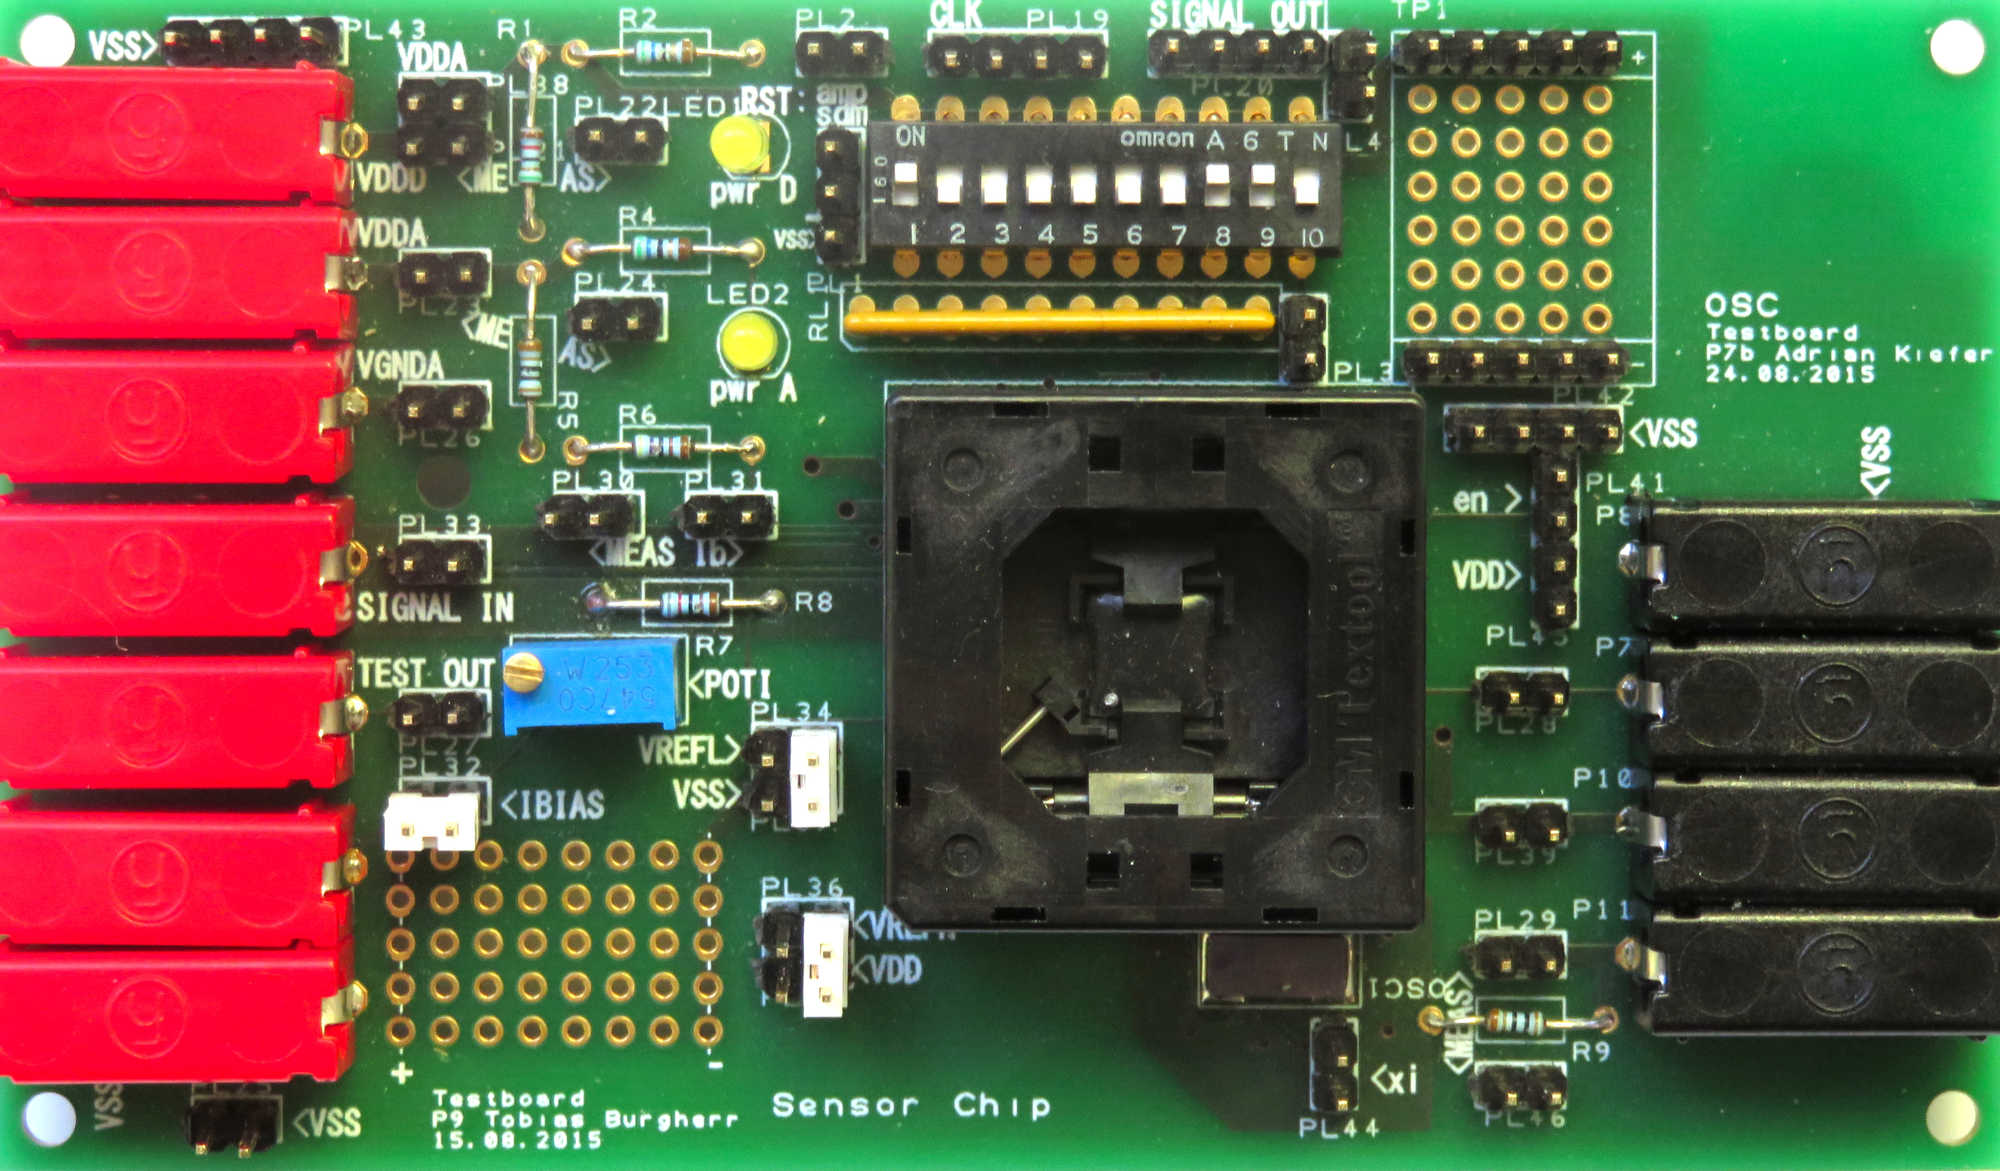
\includegraphics[width=\textwidth]{images/pcb/pcbOverview.jpeg}
%    \newcommand{\plugtext}[1]{\textbf{\texttt{\Large{#1}}}}

\begin{tikzpicture}
    \begin{scope}[x={(0mm,135mm)},y={(0mm,79mm)},line width=1pt,cap=round]
        \node[anchor=south west,inner sep=0mm] at (0mm,0mm) {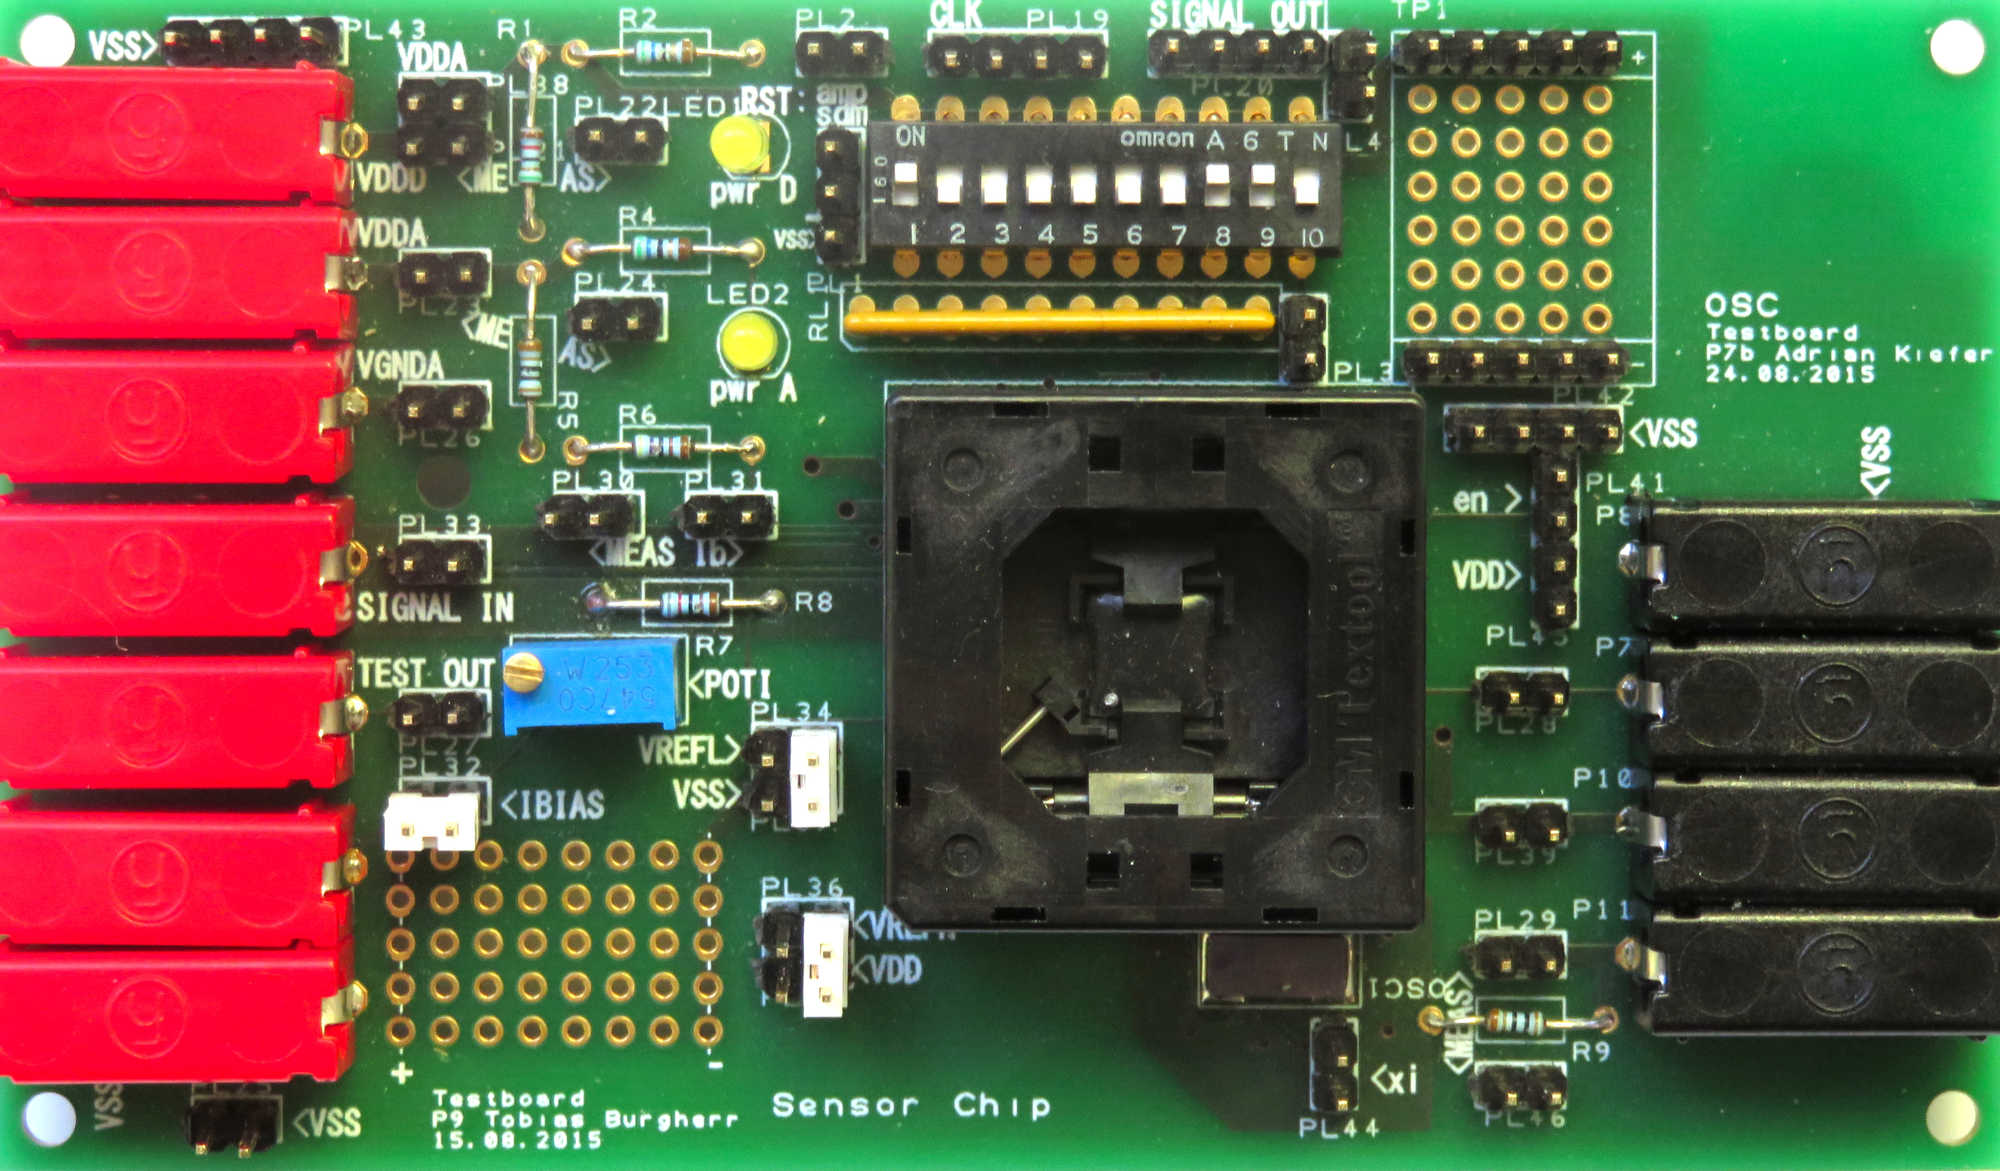
\includegraphics[width=135mm]{images/pcb/pcbOverview.jpeg}};
    \end{scope}
    %\node[fill=black,text=white,anchor=south west] at (0mm,0mm) {\textsf{\Large{VDDD}}};

    \node[%
        %fill=black,
        %fill opacity=0.5,
        text=white,
        text opacity=1,
        rounded corners=1mm,
        anchor=south west] at (4mm,66mm) {\plugtext{VDDD}};

    \node[%
        %fill=black,
        %fill opacity=0.5,
        text=white,
        text opacity=1,
        rounded corners=1mm,
        anchor=south west] at (4mm,56.5mm) {\plugtext{VDDA}};

    \node[%
        %fill=black,
        %fill opacity=0.5,
        text=white,
        text opacity=1,
        rounded corners=1mm,
        anchor=south west] at (4mm,47.5mm) {\plugtext{VGNDA}};

    \node[%
        %fill=black,
        %fill opacity=0.5,
        text=white,
        text opacity=1,
        rounded corners=1mm,
        anchor=south west] at (1mm,37.5mm) {\textbf{\textsf{\large{SIGNAL IN}}}};

    \node[%
        %fill=black,
        %fill opacity=0.5,
        text=white,
        text opacity=1,
        rounded corners=1mm,
        anchor=south west] at (1mm,27.5mm) {\textbf{\textsf{\large{TEST OUT}}}};

    \node[%
        %fill=black,
        %fill opacity=0.5,
        text=white,
        text opacity=1,
        rounded corners=1mm,
        anchor=south west] at (4mm,17mm) {\plugtext{IBIAS}};

    \node[%
        %fill=black,
        %fill opacity=0.5,
        text=white,
        text opacity=1,
        rounded corners=1mm,
        anchor=south west] at (4mm,8mm) {\plugtext{VSS}};
\end{tikzpicture}

%    \caption{Test board overview with its most commonly used connections labeled}
%    \label{fig:pcbOverview}
%\end{figure}
%
%\begin{figure}
%    \centering
%    \missingfigure{Raspberry Pi}
%    \caption{The Raspberry Pi used in this setup}
%    \label{fig:raspi}
%\end{figure}
%
%The chip's top  level pins are listed in  \tref{tab:inputPlugs}. Some of these
%can  be configured  via an  array of  DIP switches,  located between  the chip
%socket  and  the  \signal{CLK}  and  \signal{SIGNAL OUT}  plugs  on  the  test
%board. The most commonly  used among these is the preamp's  gain, which can be
%set to values between \num{-16}  and \num{+16}. The preamp's sign (positive or
%negative) is  a dedicated  switch; its  gain's absolute  values are  listed in
%\tref{tab:dipGain}.
%
%\begin{table}
%    \centering
%    \caption{Sensor chip toplevel pins}
%    \label{tab:inputPlugs}
%    \scriptsize
%    \sisetup{list-pair-separator = { or }}
%    \rowcolors{2}{solarized-base3}{white}
%    \begin{tabular}{>{\fontfamily{jkptt}\selectfont}l>{\fontfamily{jkptt}\selectfont}lp{30mm}lp{30mm}} \\
%    %\begin{tabular}{>{\fontfamily{lmtt}\selectfont}l>{\fontfamily{lmtt}\selectfont}lp{30mm}lp{30mm}} \\
%        \toprule
%        \textnormal{\textsc{Pin \#}} & \textnormal{\textsc{Name}}                  & \textsc{Description} & \textsc{Value} & \textsc{Note} \\
%        \midrule
%        39 & vin                     & analog input signal                         & \SIrange{0.5}{2.5}{\volt} & \\
%        25 & bit\_stream             & digital output signal                       & \SIlist{0;3}{\volt}       & \\
%        34 & clk                     & clock                                       & \SIlist{0;3}{\volt}       & \\
%        36 & sdm\_rst                & pulse to reset the $\Sigma\Delta M$         & \SIlist{0;3}{\volt}       & short pulse is enough (min $T_C$) \\
%        41 & vgnda                   & analog ground                               & \SI{1.5}{\volt}           & \\
%        48 & vrefh                   & high reference voltage                      & \SI{3}{\volt}             & \\
%        47 & vrefl                   & low reference voltage                       & \SI{0}{\volt}             & \\
%        46 & ibias                   & bias current                                & \SI{120}{\micro\ampere}   & $24 \cdot 5 \cdot 1$, internally reduced by 120 \\
%        43 & sc\_amp\_vout\_test\_en & enables test output after preamp            & \SIlist{0;3}{\volt}       & \SI{0}{\volt}: off, \SI{3}{\volt}: on\\
%        44 & sc\_amp\_vout\_test     & test output after preamp                    & \SIrange{0.5}{2.5}{\volt} \\
%        33 & sc\_amp\_rst\_ext\_en   & enables external reset input for the preamp & \SIlist{0;3}{\volt}       & \SI{0}{\volt}: off, \SI{3}{\volt}: on\\
%        32 & sc\_amp\_rst\_ext       & external reset input for the preamp         & \SIlist{0;3}{\volt}       & Internally synced to \signal{clk}. Needs \signal{en} signal. \\
%        35 & sc\_amp\_pos\_neg\_amp  & positive or negative gain                   & \SIlist{0;3}{\volt}       & \SI{0}{\volt}: positive, \SI{3}{\volt}: negative \\
%        28 - 31 & sc\_amp\_csel<3:0> & set gain                                    & \SIlist{0;3}{\volt}       & See table TODO \\
%        27 & sc\_amp\_en             & enable preamp                               & \SIlist{0;3}{\volt}       & \SI{0}{\volt}: off, \SI{3}{\volt}: on\\
%        26 & sah\_sdm\_en            & enable $\Sigma\Delta M$ S/H bock            & \SIlist{0;3}{\volt}       & \SI{0}{\volt}: off, \SI{3}{\volt}: on\\
%        42 & vdda                    & analog positive power supply                & \SI{3}{\volt}             & \\
%        37 & vddd                    & digital positive power supply               & \SI{3}{\volt}             & \\
%        40 & vss                     & analog and digital negative power supply    & \SI{0}{\volt}             & \\
%        \bottomrule
%    \end{tabular}
%    \sisetup{list-pair-separator = { and }}
%\end{table}
%
%\begin{table}
%    \centering
%    \caption{DIP switch settings for amplifier gain}
%    \label{tab:dipGain}
%    \scriptsize
%    \begin{tabular}{%
%            >{\fontfamily{jkptt}\selectfont}r
%            >{\fontfamily{jkptt}\selectfont}r
%            >{\fontfamily{jkptt}\selectfont}r
%            >{\fontfamily{jkptt}\selectfont}r|
%            >{\fontfamily{jkptt}\selectfont}r}
%        \toprule
%        \signal{sc\_amp\_en(3)} &
%        \signal{sc\_amp\_en(2)} &
%        \signal{sc\_amp\_en(1)} &
%        \signal{sc\_amp\_en(0)} &
%        Gain \\
%        \midrule
%        1 & 1 & 1 & 1 &  1 \\
%        0 & 1 & 1 & 1 &  2 \\
%        0 & 0 & 1 & 1 &  4 \\
%        0 & 0 & 1 & 1 &  8 \\
%        0 & 0 & 0 & 1 & 16 \\
%        \bottomrule
%    \end{tabular}
%\end{table}
%
%
%% ---------------------------------------------------------------------------- %
%\clearpage
%\section{Putting the Sensor IC Into Operation}
%\label{sec:ICintoOperation}
%% ---------------------------------------------------------------------------- %
%
%This  section  will  detail  the  steps  needed to  put  the  Sensor  IC  into
%operation. Some  of  this  information  will be  redundant  with  the  reports
%\cite{ref:burgherr},  \cite{ref:gloor} and  \cite{ref:baier},  but  we aim  to
%provide a  convenient guide for this  process in a single  place, thus sparing
%future teams the effort of needing  to assemble this information from multiple
%sources, which is both a time-consuming and error-prone process.
%\todo[noline]{Make direct references to pages/tables in other reports?}
%\todo[noline]{Safety precations}
%
%Fundamentally, putting the chip into operation consists of the following steps:
%\begin{itemize}\tightlist
%    \item
%        Set up \raspi.
%    \item
%        Determine bias resistor setting.
%    \item
%        Set   DIP   switches   to   the  appropriate   values   according   to
%        \tref{tab:dipGain}.
%    \item
%        Connect supply voltages and bias current supply.
%    \item
%        Connect \raspi~and test board.
%\end{itemize}
%
%% ---------------------------------------------------------------------------- %
%\subsection{Setting up the Raspberry Pi}
%\label{subsec:raspiInstall}
%% ---------------------------------------------------------------------------- %
%
%\todo[inline]{%
%    Give a more detailled guide on what to install on the \raspi~ and how than
%    in the previous reports
%}
%
%\todo[inline]{RaspiPower supply}
%\todo[inline]{External connections for Raspi}
%\todo[inline]{%
%    Controlling the  function generator  for \signal{SIGNAL  IN} line  via the
%    \raspi.
%}
%
%% ---------------------------------------------------------------------------- %
%\subsection{Hardware Setup}
%\label{subsec:hardwareSetup}
%% ---------------------------------------------------------------------------- %
%
%Operating the test board requires the following components:
%
%\begin{itemize}\tightlist
%    \item
%        direct voltage source: \SI{3}{\volt}
%    \item
%        direct voltage source: \SI{1.5}{\volt}
%    \item
%        Direct  current  source: \SI{120}{\micro\ampere}.  \emph{Note:} If  no
%        direct current source  is available, as in our case,  a direct voltage
%        source in combination with  a multimeter for controlling/measuring the
%        current can be used.
%    \item
%        function generator for \signal{clk}
%    \item
%        Direct  and  alternating  voltage  source  for  input  signal  voltage
%        (between \SI{0.5}{\volt} and \SI{2.5}{\volt}).
%    \item
%        An oscilloscope for monitoring the preamp's output on the \signal{TEST
%        OUT} pin, as well as the raw bit stream.
%\end{itemize}
%
%The complete setup is depicted in \fref{fig:experimentDiagram}.
%
%\begin{figure}
%    \sisetup{range-phrase = { \ldots }}
\sisetup{list-pair-separator = {/}}

\begin{circuitikz}[x=1mm,y=1mm]

    % ------------------------------------------------------------------------ %
    % Test Board
    % ------------------------------------------------------------------------ %
    \draw (0,0) -- (50,0) -- (50,29) -- (0,29) -- cycle;

    % Left-hand side Plugs
    \foreach \y in {0,...,6} {%
        \draw (0,\y*3.5+2.5) -- (8,\y*3.5+2.5) -- (8,\y*3.5+5.5) -- (0,\y*3.5+5.5) -- cycle;
    };

    % CLK plug
    \draw (23,27.5) -- (27,27.5) -- (27,28.5) -- (23,28.5) -- cycle;
    \foreach \x in {0,...,3} {%
        \fill (23.25+\x,27.75) -- (23.25+\x+0.5,27.75) -- (23.25+\x+0.5,28.25) -- (23.25+\x,28.25) -- cycle;
    }

    % Signal out Plug
    \draw (29,27.5) -- (33,27.5) -- (33,28.5) -- (29,28.5) -- cycle;
    \foreach \x in {0,...,3} {%
        \fill (29.25+\x,27.75) -- (29.25+\x+0.5,27.75) -- (29.25+\x+0.5,28.25) -- (29.25+\x,28.25) -- cycle;
    }

    % DIP switch housing
    \draw (22,24) -- (32,24) -- (32,26) -- (22,26) -- cycle;
    \foreach \x in {1,...,9} {%
        \draw (\x+22,24) -- (\x+22,26);
    }

    % DIP Switches
    \foreach \x in {0,...,9} {%
        \fill (22+\x+0.25,24.5) -- (22+\x+0.75, 24.5) -- (22+\x+0.75,25) -- (22+\x+0.25,25) -- cycle;
    }


    % ------------------------------------------------------------------------ %
    % RasPi
    % ------------------------------------------------------------------------ %
    \draw (10,50) -- (50,50) -- (50,70) -- (10,70) -- cycle;

    % GPIO
    \foreach \x in {0,...,39} {%
        \fill (49.5-\x*0.6667-0.25,50.25) -- (49.5-\x*0.66675-0.25-0.35,50.25) -- (49.5-\x*0.66675-0.25-0.35,50.5) -- (49.5-\x*0.6667-0.25,50.5);
        \fill (49.5-\x*0.6667-0.25,50.875) -- (49.5-\x*0.66675-0.25-0.35,50.875) -- (49.5-\x*0.66675-0.25-0.35,51.125)   -- (49.5-\x*0.6667-0.25,51.125);
    }

    % ------------------------------------------------------------------------ %
    % Voltage and Current Sources
    % ------------------------------------------------------------------------ %

    % Supply Voltages
    \draw (0,25) -- (-5,25) node[circ] {}-- (-20,25) to[american voltage source,l_=\scriptsize{\SI{3}{\volt}},-*] (-20,40);

    \draw (-5,25) -- (-5,21.5) -- (0,21.5);
    \draw (0,18) -- (-40,18) to[american voltage source,l_=\scriptsize{\SI{1.5}{\volt}},-*] (-40,40);

    \draw (-60,40) to[american current source,l^=\scriptsize{\SI{120}{\micro\ampere}},*-] (-60,11) -- (0,11);

    % GND Line
    \draw (0,4) -- (-70,4) -- (-70,40) -- (25.125,40) -- (25.125,50.25);

    % CLK
    \draw (0,40) node[circ]{} -- (0,35) to[square voltage source,-*] (23.5,35) -- (23.5,28);
    \draw (23.5,35) -- (28.375,35) -- (28.375,50.25);

    % ------------------------------------------------------------------------ %
    % Signal out line
    % ------------------------------------------------------------------------ %
    \draw (30.5,28) -- (30.5,50.25);


    \draw (-70,4) node[ground]{} node[circ]{};

    %\foreach \ini [evaluate=\ini as \inieval using 2*\ini] in {0,...,6}
    %\draw[ultra thick,cyan] (\inieval,0) -- ++(0,1) -| (\inieval+1,0) -- (\inieval+2,0);
\end{circuitikz}


%    \caption{%
%        Experimental setup  with connections.  \emph{Note}: Drawing not
%        finalized yet.%
%    }
%    \label{fig:experimentDiagram}
%\end{figure}
%
%The  voltage  on  the  bias  input  must be  set  so  that  the  bias  current
%is  \SI{120}{\micro\ampere}. The  current  can  be adjusted  with  a  variable
%resistor. \cite{ref:burgherr} outlines how the  value for this resistor can be
%calculated. To ensure correct  operation, it is highly  recommended to monitor
%the current on the bias input pin  with a current meter and adjust the voltage
%source as needed to  achieve a current of \SI{120}{\micro\ampere}.\todo{actual
%R/V values used in our experiments}
%% Burgherr: I-32: Bias current
%
%Additionally, we strongly advise validating the  DC input voltages with a volt
%meter and not blindly trusting the given voltage source's indicator.
%
%The final setup, as used in the experiments for this report, is depicted in \fref{fig:completeSetup}.
%
%\begin{figure}
%    \missingfigure{Complete setup as used in the experiments for this report (photograph, not diagram)}
%    \caption{the setup as used in the experiments for this report}
%    \label{fig:completeSetup}
%\end{figure}
%
%An \emph{Aim TTi MX100TP} laboratory  DC power supply (\fref{fig:dcSupply}) is
%used  as input  for the  \SI{3}{\volt}, \SI{1.5}{\volt}  and the  bias current
%lines.
%
%\begin{figure}
%    \missingfigure{DC Power Supply}
%    \caption{DC Power Supply}
%    \label{fig:dcSupply}
%\end{figure}
%
%The  bias  current  is  monitored with  an  \emph{Agilent  U1253B}  multimeter
%(\fref{fig:agilentMultimeter}),  while   a  \emph{Keysight   34465A}  tabletop
%(\fref{fig:keysightMultimeter})  multimeter is  used for  measuring the  input
%signal voltage (in order not stay within the sensible range of \SI{0.5}{\volt}
%and \SI{2.5}{\volt},  below and  above which  the ADC  enters saturation). The
%output  bitstream   is  monitored   with  a  \emph{LeCroy   waveRunner  6100A}
%oscilloscope.
%
%\begin{figure}
%    \missingfigure{DC Power Supply}
%    \caption{DC Power Supply}
%    \label{fig:agilentMultimeter}
%\end{figure}
%
%\begin{figure}
%    \missingfigure{Keysight Multimeter}
%    \caption{Keysight tabletop multimeter}
%    \label{fig:keysightMultimeter}
%\end{figure}
%
%\begin{figure}
%    \missingfigure{LeCroy Oscilloscope}
%    \caption{LeCroy Oscilloscope}
%    \label{fig:lecroyOscilloscope}
%\end{figure}
%
%Two    \emph{Hewlett   Packard    33120A}   arbitrary    waveform   generators
%(\fref{fig:HPwave}) are used  to provide the system's clock  and input signal,
%respectively. The device  used for generating  the input signal  is controlled
%remotely  via the  \raspi\todo{Document  Python scripts  used for  this}. This
%reduces the  time required  for performing  experiments significantly. Further
%efficiency gains  could be made by  replacing the DIP switches  with something
%which can be controlled remotely (the only thing requiring manual intervention
%at  that point  would  be the  replacing  of the  chip  itself when  measuring
%multiple samples).
%
%\begin{figure}
%    \missingfigure{Hewlett Packard Arbitrary Waveform Generator}
%    \caption{Hewlett Packard Arbitrary Waveform Generator}
%    \label{fig:HPwave}
%\end{figure}
%
%Appendix \ref{sec:HPwave}  details the configuration process  for the function
%generator, starting on page \pageref{sec:HPwave}.

% --------------------------------------------------------------------------- %
\chapter{Measurement and Data Processing}
\label{chap:measurementProcess}
% --------------------------------------------------------------------------- %

\todo[inline]{%
    Primary questions to answer in this chapter: What did we measure, how, and
    why?
}

Two different  kinds of measurements  are performed:  Analog  measurements are
used  to assess  the  performance  of the  preamp  via  the \signal{TEST  OUT}
pin. Secondly, digital measurements for assessing the $\Sigma\Delta M$ as well
as the two components combined are derived by evaluating the bit stream.

Analog measurement data  is captured with an osccilloscope  and then evaluated
on a PC. The bit stream is captured and processed on the \raspi.

For both the  preamp as well as the $\Sigma\Delta$  modulator, DC measurements
over an input  voltage range between \SI{0.5}{\volt}  and  \SI{2.5}{\volt} are
performed. AC measurements are used to assess the system's frequency behavior.

Both DC and AC measurements are performed with various settings for the preamp
(sign,  gain,  on/off)  as  well as  the  $\Sigma\Delta$  modulator  (sampling
frequency).

The sample size is 10 chips, unless indicated otherwise.

Based on these measurements and their  analysis in the next chapter, we strive
to answer the question  of what sort of use cases this  sytem is suitable for,
and with which settings.

% TODO: noise
% TODO: resolution in bits under a given set of circumstances
% TODO: Measurement methodology


% --------------------------------------------------------------------------- %
\section{Pre-Amplifier: DC Measurements}
\label{sec:preAmpDC}
% --------------------------------------------------------------------------- %

% --------------------------------------------------------------------------- %
\section{Sigma-Delta Converter: DC Measurements}
\label{sec:sigdelDC}
% --------------------------------------------------------------------------- %

% --------------------------------------------------------------------------- %
\section{Complete System: DC Measurements}
\label{sec:systemDC}
% --------------------------------------------------------------------------- %

% --------------------------------------------------------------------------- %
\section{Pre-Amplifier: AC Measurements}
\label{sec:preAmpAC}
% --------------------------------------------------------------------------- %

% --------------------------------------------------------------------------- %
\section{Sigma-Delta Converter: AC Measurements}
\label{sec:sigdelAC}
% --------------------------------------------------------------------------- %

% --------------------------------------------------------------------------- %
\section{Complete System: AC Measurements}
\label{sec:systemAC}
% --------------------------------------------------------------------------- %

% ---------------------------------------------------------------------------- %
\chapter{Results}
\label{chap:results}
% ---------------------------------------------------------------------------- %


\begin{itemize}\tightlist
    \item
        Saturation: Lower boundary: bitstream without any input signal
    \item
        Saturation: Upper boundary: Find meaningful equivalent to "no input" at lower boundary
    %\item
    %    Why do we perform DC measurements? (linearity, offset)
    %\item
    %    Why do we  perform AC measurements w/ harmonics? (What  sort of system
    %    can be measured with this chip, how fast is the plant?)
    %\item
    %    Why do we perform SNR measurements?
    \item
        What are potential  measurements which might be of  interest but which
        we  could  not perform  (and  the  reasons  for  which they  were  not
        performed)?
    \item
        What would need to be done to be able to perform those measurements?
    %\item
    %    What kind of measurements were \emph{not} performed, and why?
    %\item
    %    Which measurements were performed?
    %\item
    %    Why are these measurements relevant?
    %\item
    %    What kind of results are we expecting? (Simulation results)
    %\item
    %    What are our actual results?
    %\item
    %    What are potential causes for the differences? (Potentially split this off
    %    into a separate chapter titled \emph{Analysis} or something similar.)
\end{itemize}

%

% --------------------------------------------------------------------------- %
\section{Pre-Amplifier: DC Measurements}
\label{sec:preAmpDC}
% --------------------------------------------------------------------------- %

The preamplifier was directly  measured, isolated from the \sdm, by applying a
number of constant voltages on the input and recording the output voltage with
an oscilloscope on the \signal{TEST OUT} pin.

Since the  preamp  uses  a  switching  capacitor  implementation,  the  output
waveform is of  course  a  square  wave  of  sorts,  as  can be seen in figure
\ref{fig:preamp_waveform}.

\begin{figure}
    \centering
    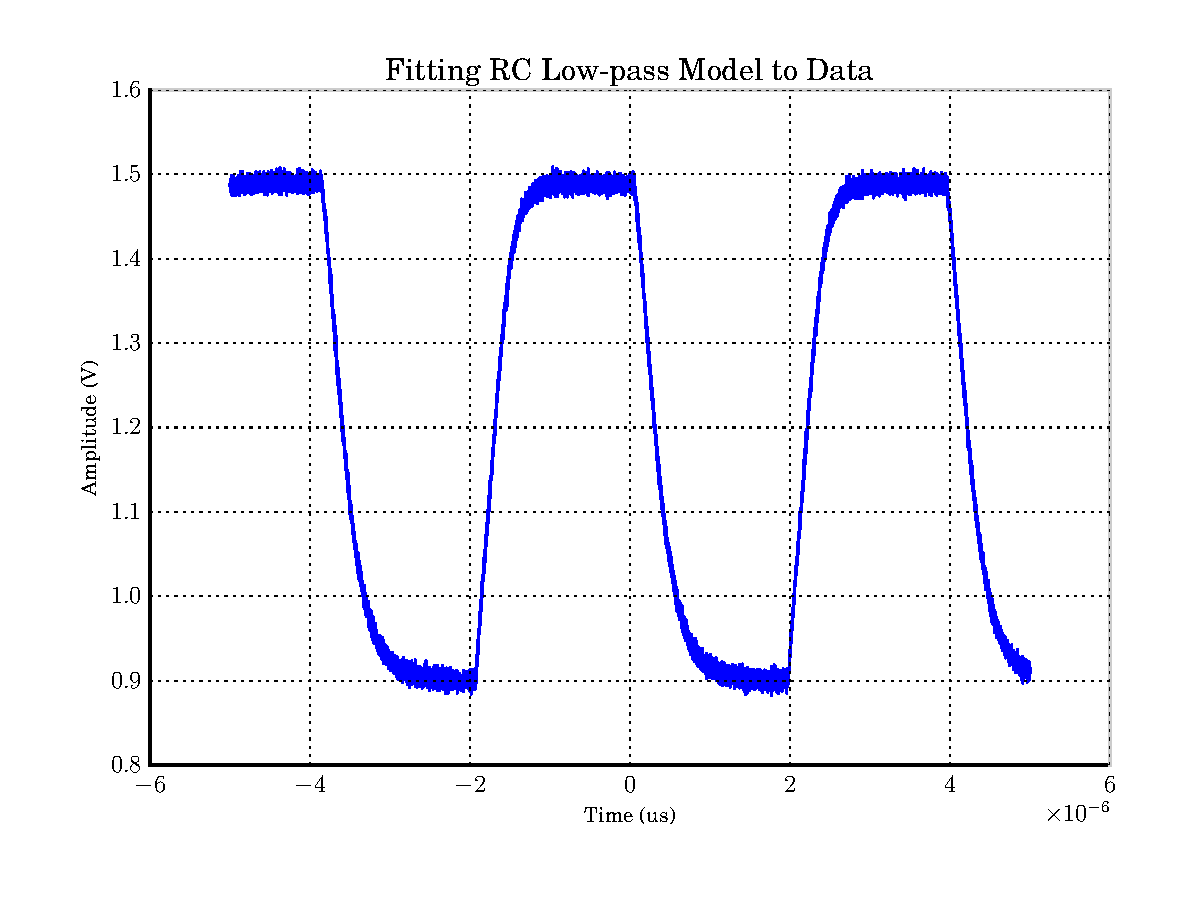
\includegraphics[width=\linewidth]{images/plots/preamp_waveform.pdf}
    \caption{Typical preamp output signal as measured on the \signal{TEST OUT} pin.}
    \label{fig:preamp_waveform}
\end{figure}

A first observation to make are the slow rise and fall-times. Indeed,  this is
one  of the major limiting factors of the chip's performance;  If  the  target
voltage can't be reached within half of the clock period (before it  is  reset
again),  the  \sdm~will end up  converting  a  lower  voltage  than  expected.

For  every  chip,  for  every sampling frequency, for every gain, inverted and
non-inverted,  11  different  input voltages were applied and the  output  was
measured.  All  of  the  data  was  then fitted using a simple first order  RC
low-pass charge/discharge model, described by the following python code:

\begin{minted}{python}
def preamp_curve(t, amp, amp_offset, period, t_offset, duty_cycle, tau1, tau2):
    def discharge_segment(t, amp, tau):
        return amp * np.exp(-t / tau)
    def charge_segment(t, amp, tau):
        return amp * (1.0 - np.exp(-t / tau))
    t_local = (t+t_offset) % period
    t_switch = period * duty_cycle
    def preamp_curve_single():
        for t_value in t_local:
            if t_value < t_switch:
                yield charge_segment(t_value, amp, tau1) + amp_offset
            else:
                yield discharge_segment(t_value - t_switch, amp, tau2) + amp_offset
    return np.array([x for x in preamp_curve_single()])
\end{minted}

The initial parameters for the  fit  were obtained by first smoothing the data
(using  a  Savitzky-Golay  filter) and finding  the  transition  points.  This
process is illustrated  in  figure  \ref{fig:transition_detection}.  This  was
necessary because there are a lot of local minima the fit could fall into. The
initial period, duty cycle, and phase shift can be extracted from the distance
between the  transition  lines.  The  initial  amplitude  and  offset  can  be
determined with a min/max search.

\begin{figure}
    \centering
    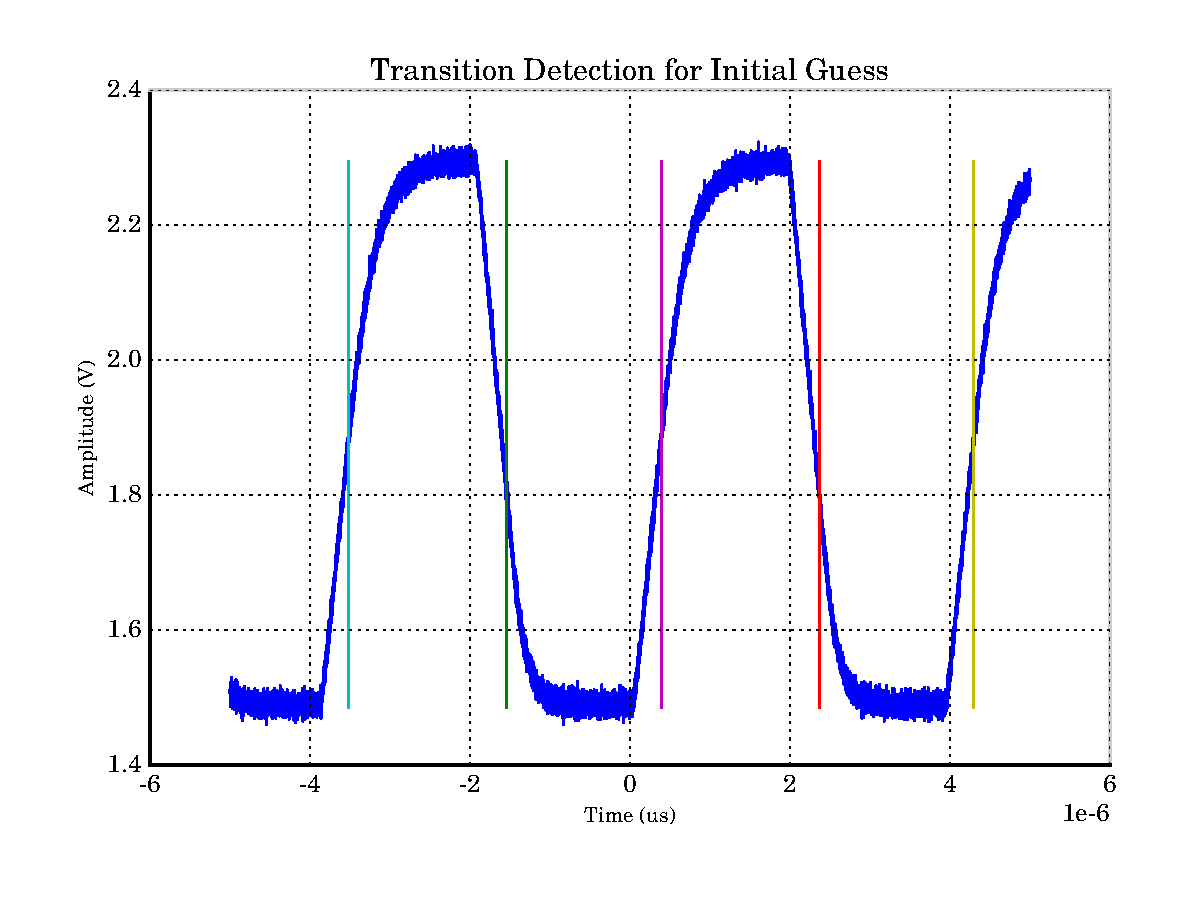
\includegraphics[width=\linewidth]{images/plots/transition-detection.pdf}
    \caption{Finding the transition points as a method to accurately estimate initial parameters for duty cycle, period and phase.}
    \label{fig:transition_detection}
\end{figure}

The  most  interesting  parameters  yielded  from  the fit  are  $\tau_1$  and
$\tau_2$, which give us a rough idea of the transconductance $g_m$ of the OTA.
The gain can also be easily extracted after  the  fit  by performing a min/max
search   on   the   fitted   curve.   This    is    illustrated    in   figure
\ref{fig:fitting_rc_model} as the horizontal line.

\begin{figure}
    \centering
    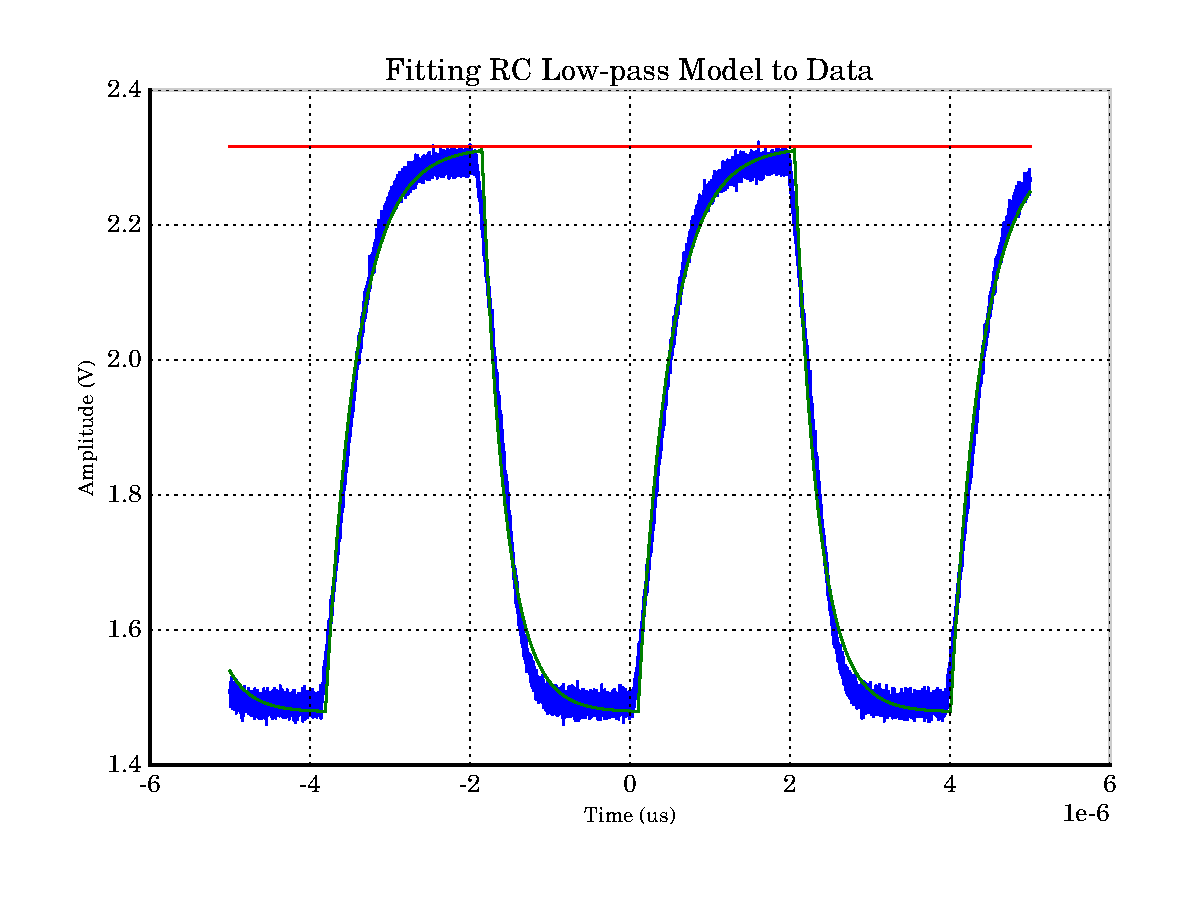
\includegraphics[width=\linewidth]{images/plots/fitting_rc_model.pdf}
    \caption{Fitting the RC model to the raw data and determining the preamp output voltage.}
    \label{fig:fitting_rc_model}
\end{figure}

It can be observed that the transconductance $g_m$ is largest  when  near  the
reference  voltage $V_{ref}=\SI{1.5}{\volt}$ and decreases with  higher  input
amplitudes. This effect  can  be  seen  in figure \ref{fig:preamp_11_signals}.
Furthermore, in the  same  figure,  one  can  observe  slewing  on  the larger
signals.  This  effect  could  be included in the fit model  above  in  future
evaluations.

\begin{figure}
    \centering
    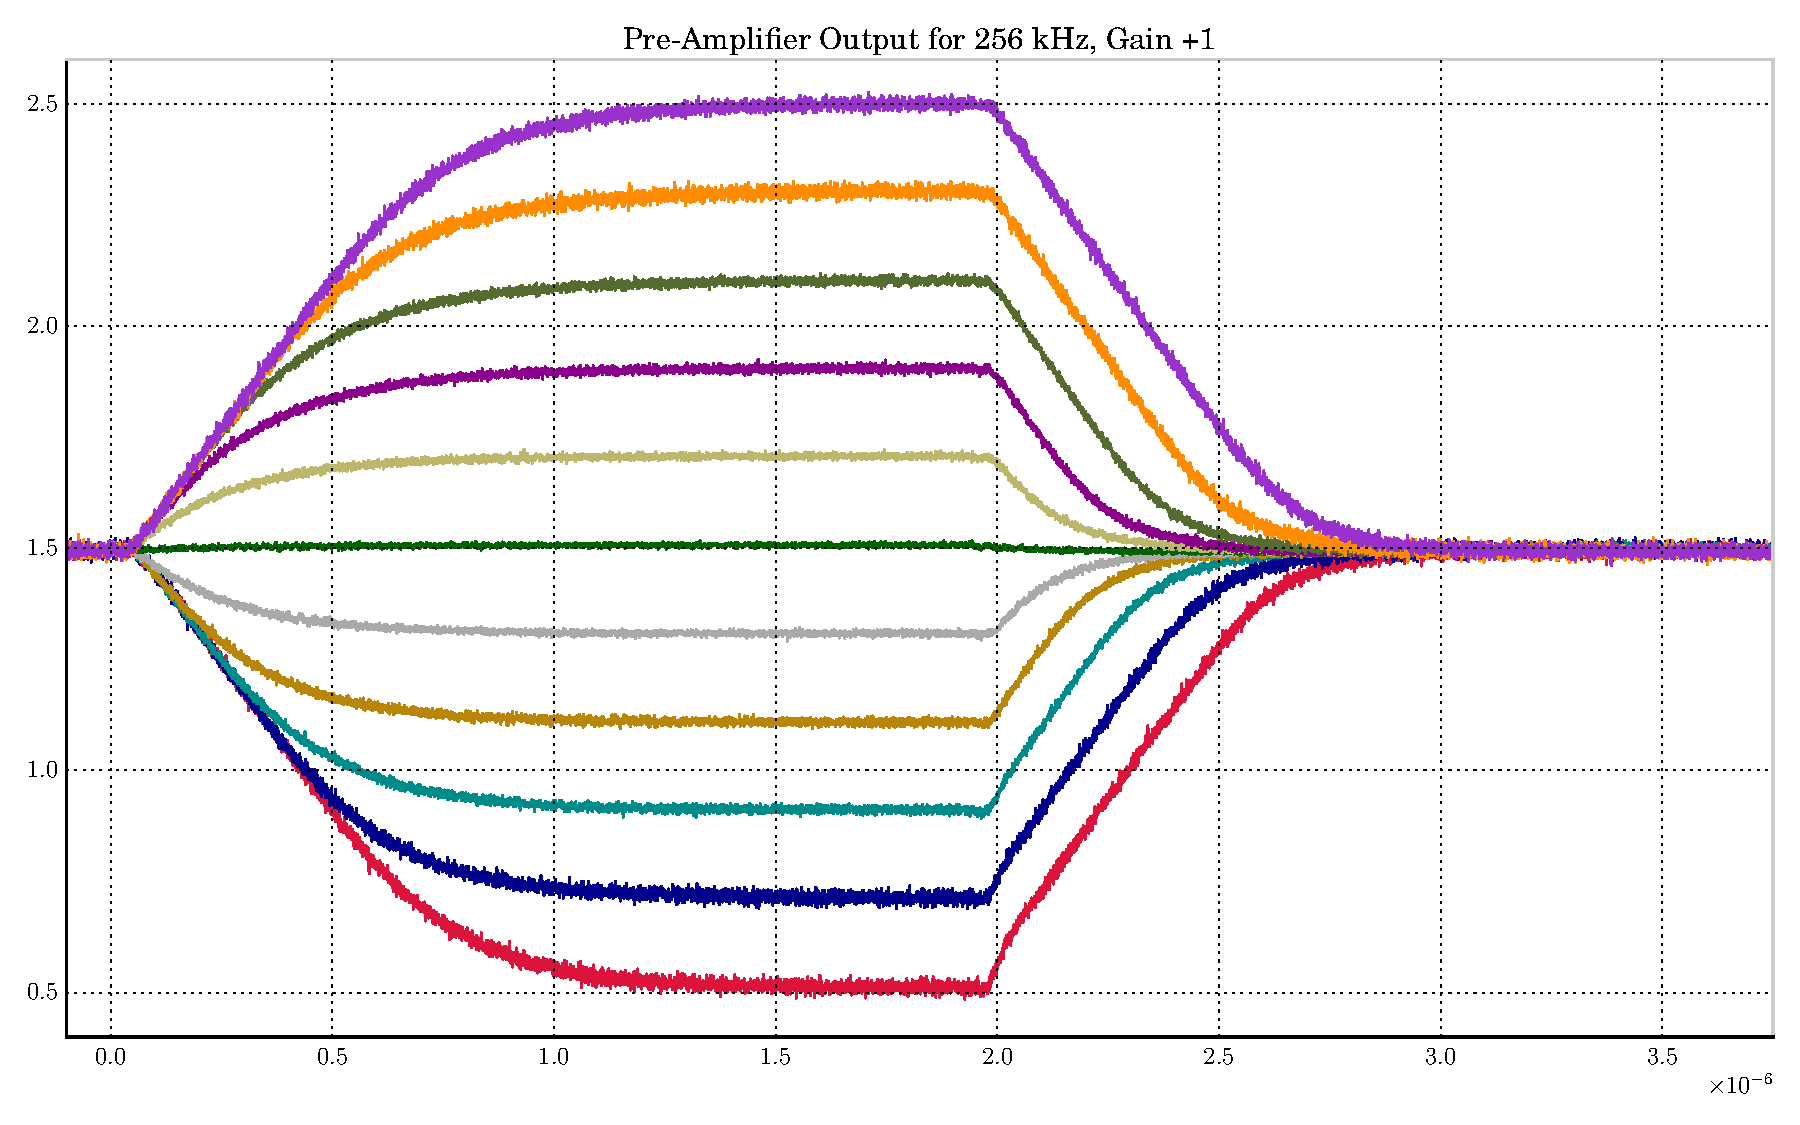
\includegraphics[width=\linewidth]{images/plots/vinComparisonPreamp.pdf}
    \caption{Output voltage of the pre-amplifier for 11 different DC input voltage levels.}
    \label{fig:preamp_11_signals}
\end{figure}
. 

By combining the individual $\tau$ constants and  plotting them in function of
the input voltage, we see the  effect of $g_m$ decreasing more clearly (figure
\ref{fig:tau}).  Here,  the  results from 10 chips were statistically averaged to get a better result.

\begin{figure}
    \centering
    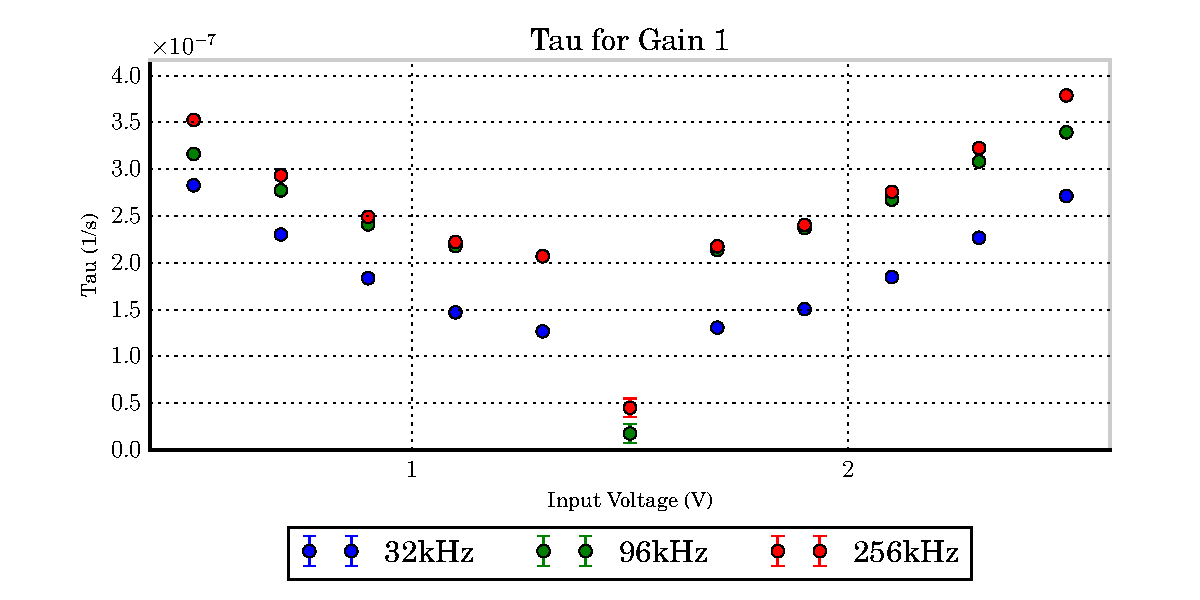
\includegraphics[width=\linewidth]{images/plots/tau_results_1.pdf}
    \caption{Fitted parameter tau (RC time constant) in function of DC input voltage.}
    \label{fig:tau}
\end{figure}

The $\tau$ constants  appear to be frequency dependent. This doesn't make much
sense and is very likely a direct  result  of  using a very rough model to fit
the data.

By  plotting  the output voltage from the preamp  in  function  of  the  input
voltage and fitting a linear function $y=mx+q$ to the data, we expect a linear
function who's  incline is equal to that of the configured gain. Additionally,
there  we expect a small offset to exist, due to the imperfections of reality.
This  process  is  visualised  in  figure \ref{fig:linear_fit}.

\begin{figure}
    \centering
    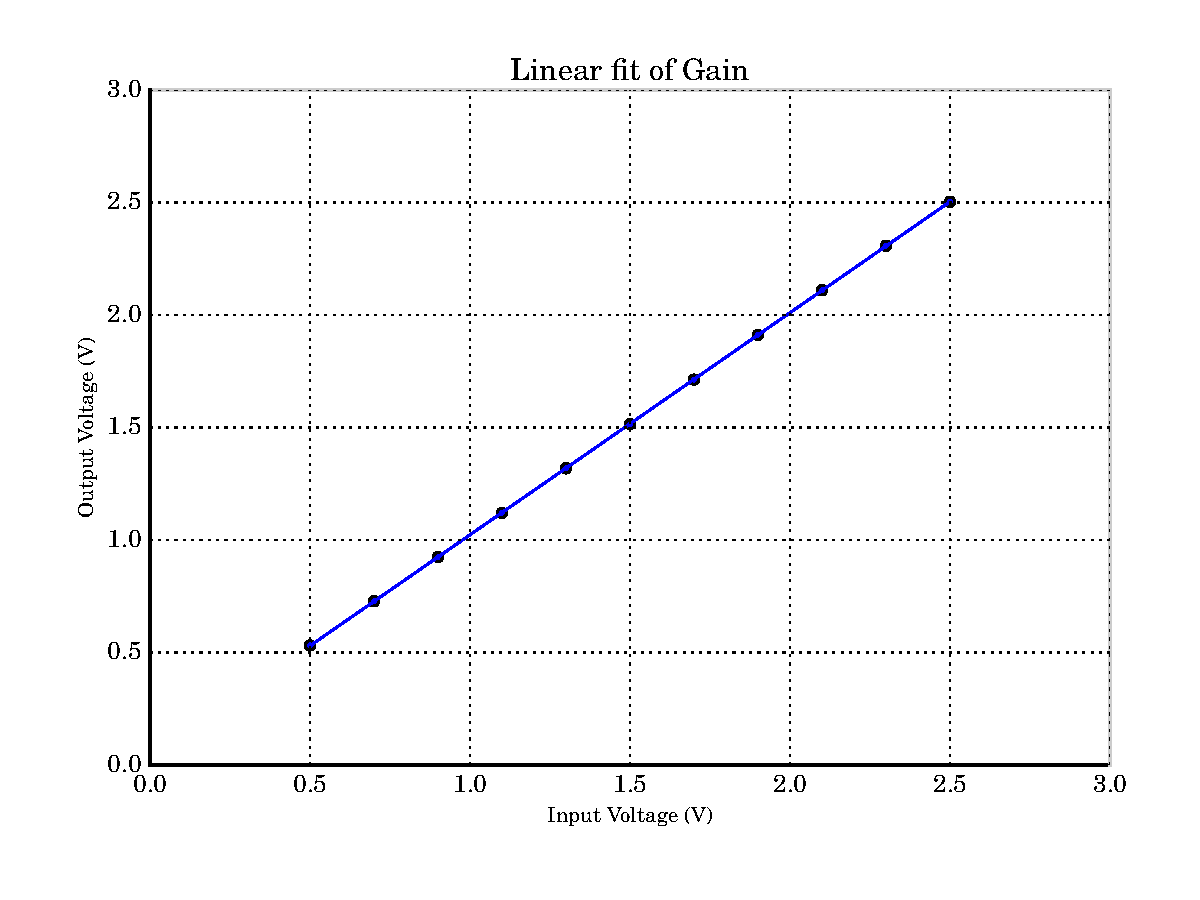
\includegraphics[width=\linewidth]{images/plots/linear_fit.pdf}
    \caption{Linear fit of DC input vs output voltage. The resulting slope is directly the effective gain.}
    \label{fig:linear_fit}
\end{figure}

\begin{figure}
    \centering
    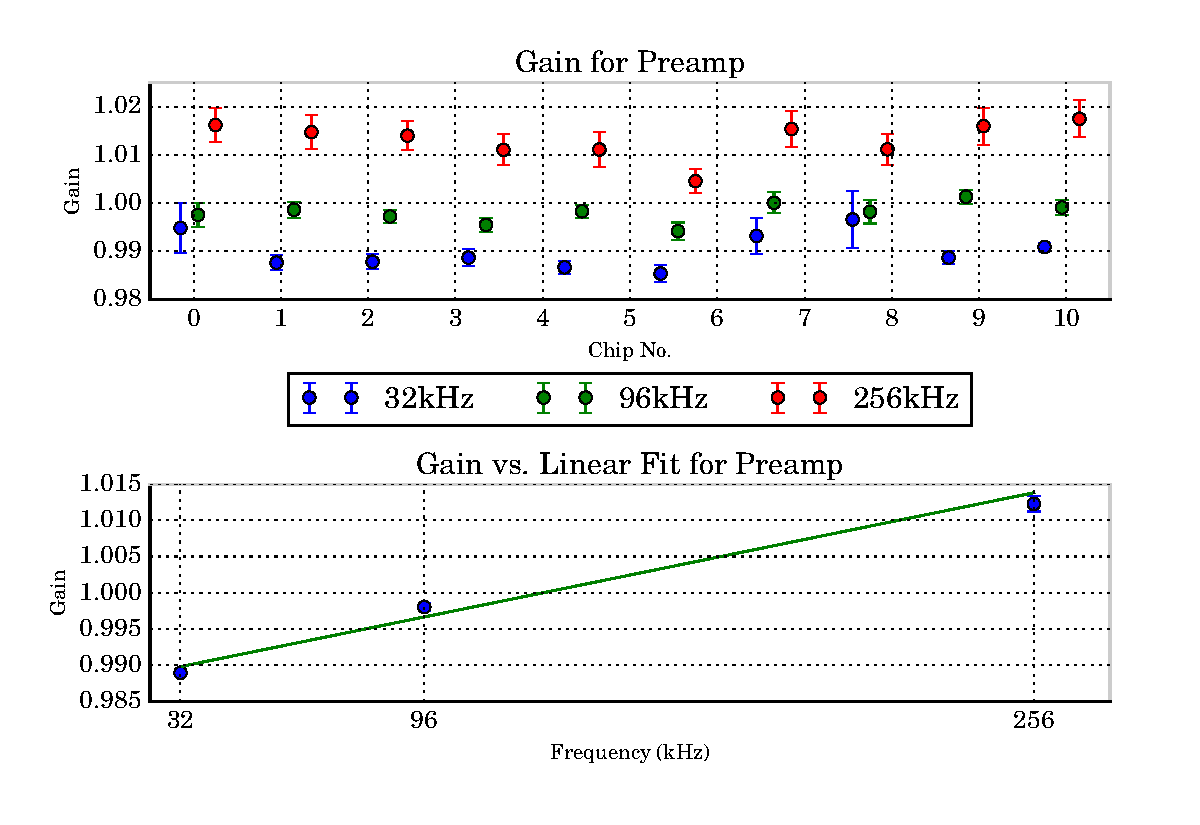
\includegraphics[width=\linewidth]{images/plots/dc_slope_preamp_gain+1.pdf}
    \caption{Effective gains of pre-amplifier at different sampling frequencies. The configured gain is 1.}
    \label{fig:preamp_slope+1}
\end{figure}
\begin{figure}
    \centering
    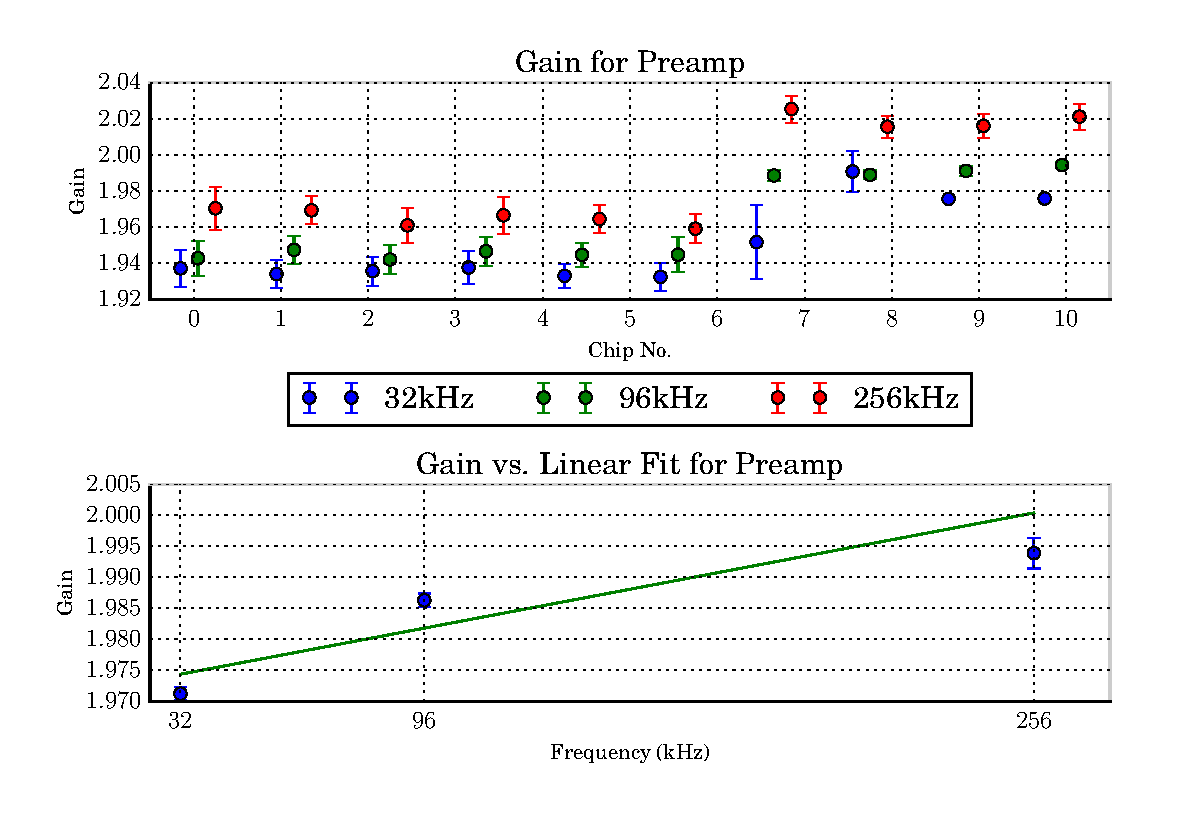
\includegraphics[width=\linewidth]{images/plots/dc_slope_preamp_gain+2.pdf}
    \caption{Effective gains of pre-amplifier at different sampling frequencies. The configured gain is 2.}
    \label{fig:preamp_slope+2}
\end{figure}
\begin{figure}
    \centering
    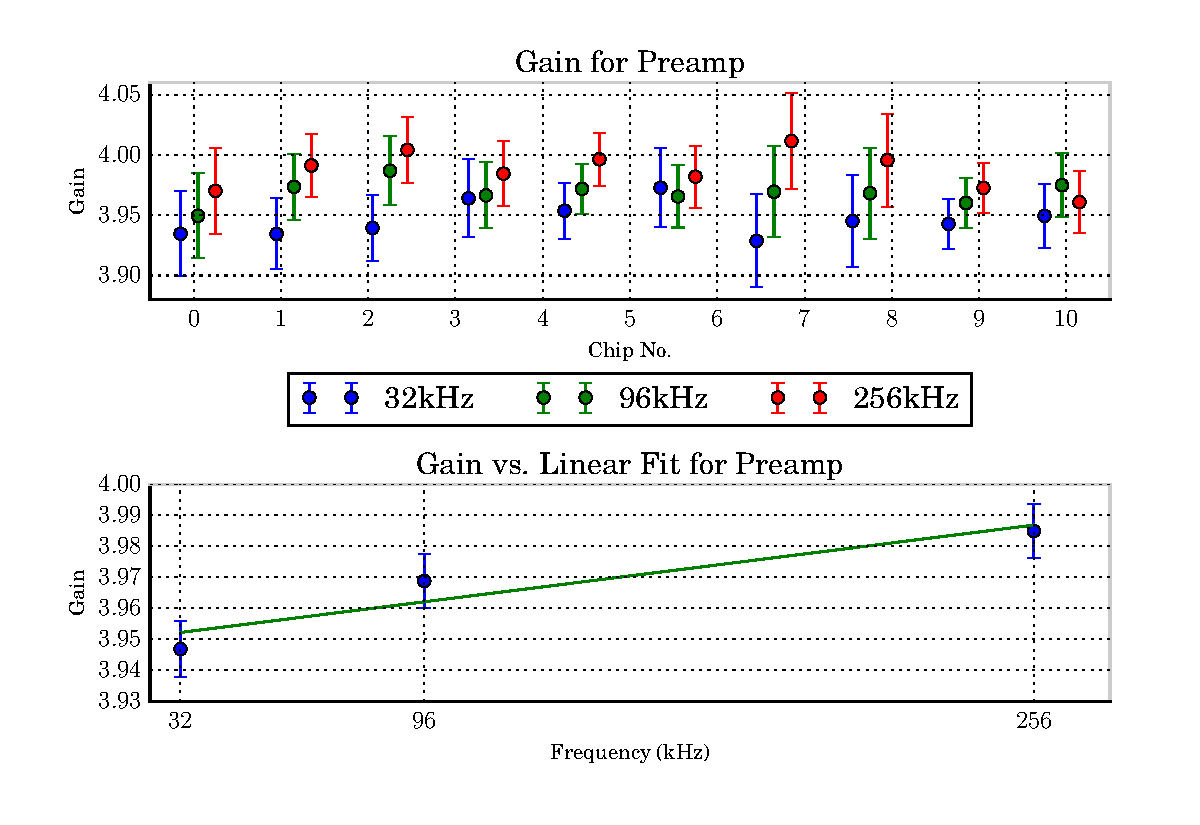
\includegraphics[width=\linewidth]{images/plots/dc_slope_preamp_gain+4.pdf}
    \caption{Effective gains of pre-amplifier at different sampling frequencies. The configured gain is 4.}
    \label{fig:preamp_slope+4}
\end{figure}
\begin{figure}
    \centering
    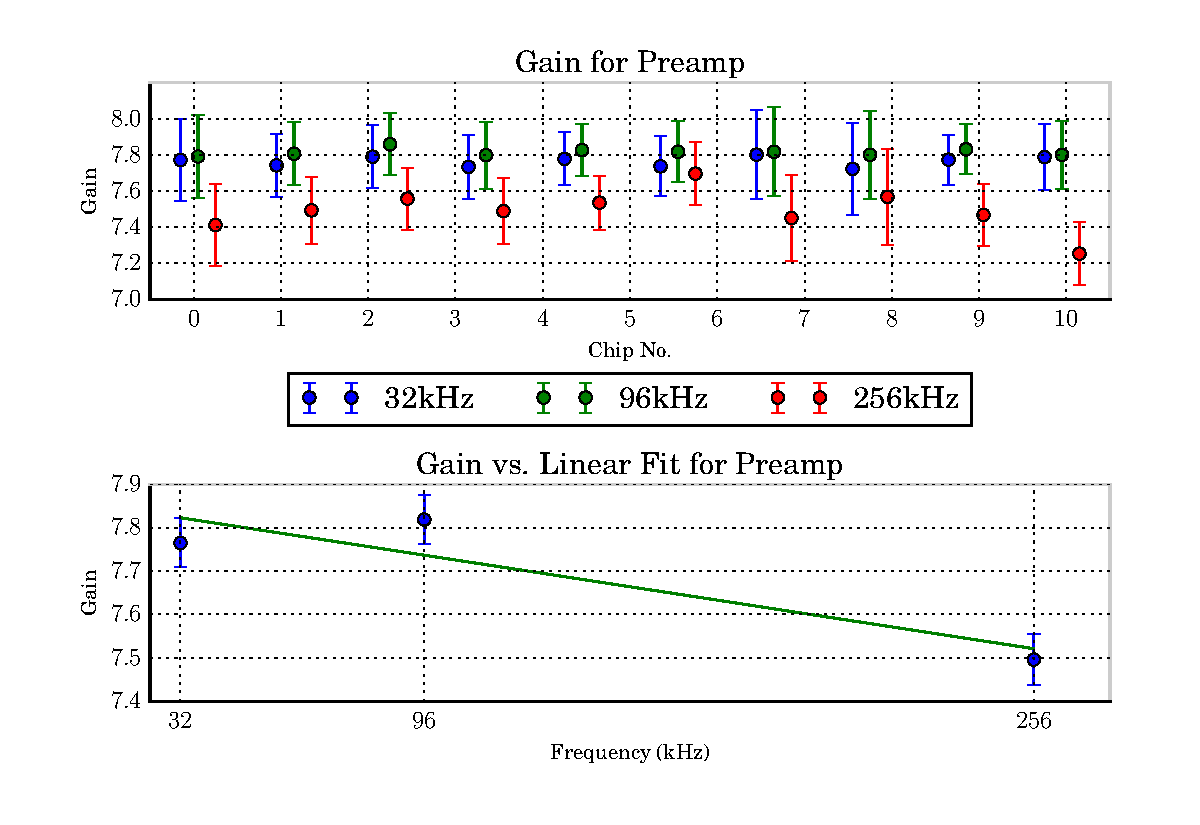
\includegraphics[width=\linewidth]{images/plots/dc_slope_preamp_gain+8.pdf}
    \caption{Effective gains of pre-amplifier at different sampling frequencies. The configured gain is 8.}
    \label{fig:preamp_slope+8}
\end{figure}
\begin{figure}
    \centering
    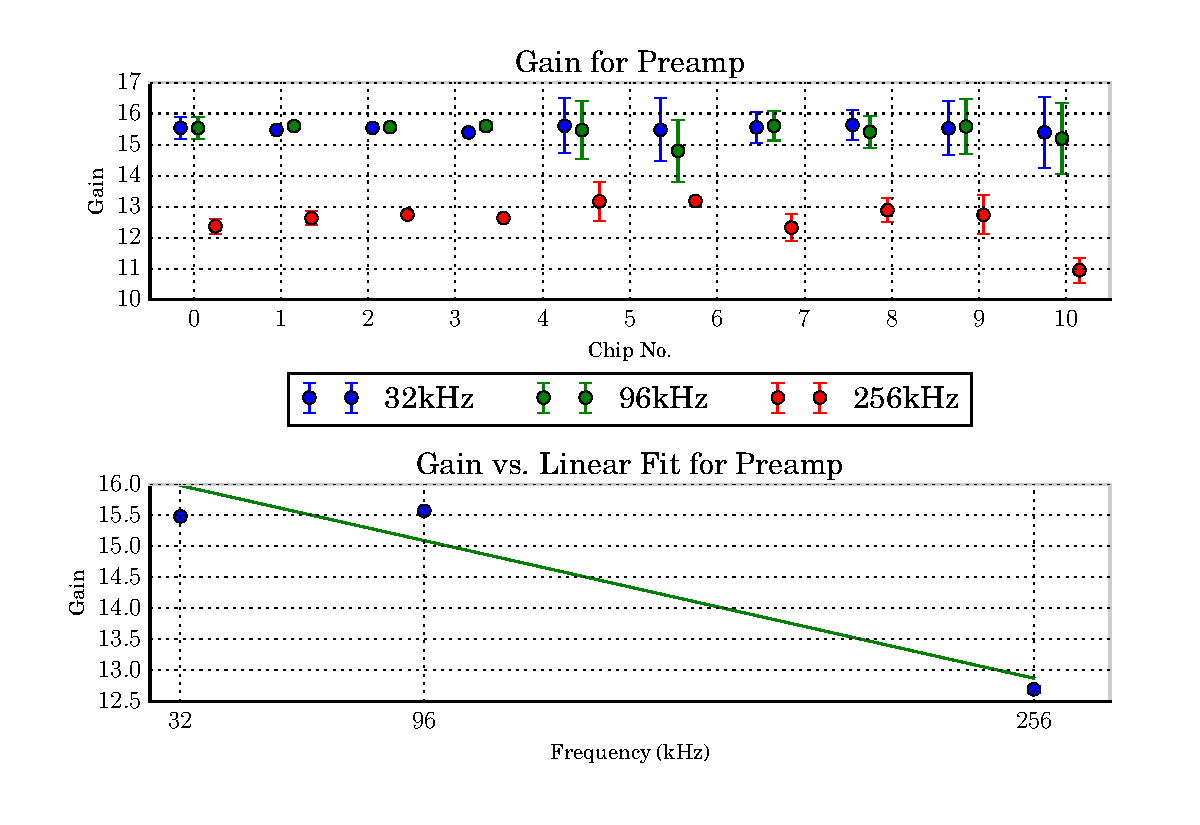
\includegraphics[width=\linewidth]{images/plots/dc_slope_preamp_gain+16.pdf}
    \caption{Effective gains of pre-amplifier at different sampling frequencies. The configured gain is 16.}
    \label{fig:preamp_slope+16}
\end{figure}

The upper plots in figures \ref{fig:preamp_slope+1}, \ref{fig:preamp_slope+2},
\ref{fig:preamp_slope+4},             \ref{fig:preamp_slope+8}             and
\ref{fig:preamp_slope+16} shows all positive  gains (1, 2, 4, 8, 16) for every
chip (x axis)  in function of $fs$. There appeared to be a correlation between
sampling frequency $fs$  and  gain,  which  made  sense  at the time, since at
higher sampling  frequencies,  the  output  of the preamp no longer manages to
properly reach the  target  voltage  in time. The lower plots in these figures
show the gain in function of sampling frequency.

It is interesting that as the configurable gain is increased, the measurements
with a higher sampling frequency decrease in expected gain. There is currently
no  explanation  as  to  why  this  is  the  case,  it   is  open  to  further
investigation.

Another interesting observation is what happens when the gain is inverted. The
same  measurements  but  for   negative   gains   can   be   seen  in  figures
\ref{fig:preamp_slope-1}, \ref{fig:preamp_slope-2},  \ref{fig:preamp_slope-4},
\ref{fig:preamp_slope-8} and  \ref{fig:preamp_slope-16}  .  This  is much more
what we expect to see: The sampling frequency and the gain have no significant
influence. It is currently unclear why the preamp behaves more correct when in
inverted  mode.   An   asymmetry   was  also  observed  while  performing  the
measurements in the lab.

\begin{figure}
    \centering
    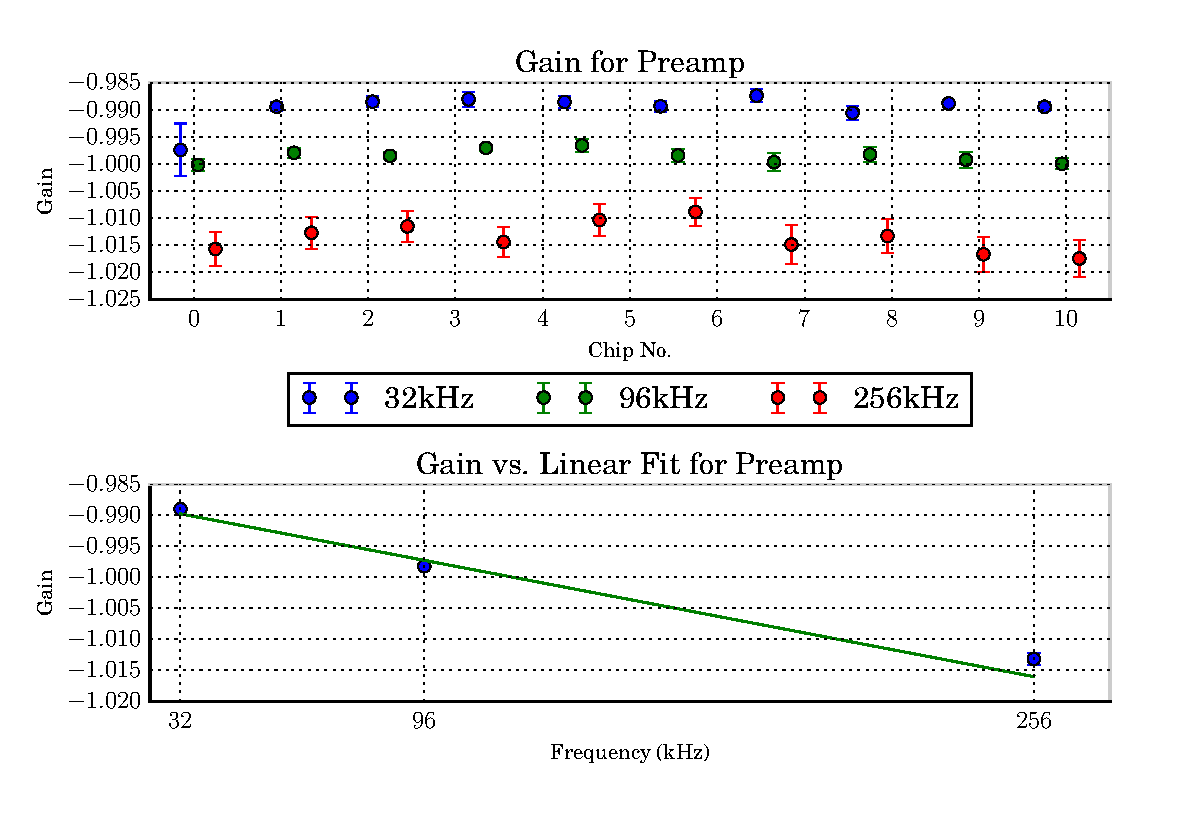
\includegraphics[width=\linewidth]{images/plots/dc_slope_preamp_gain-1.pdf}
    \caption{Effective gains of pre-amplifier at different sampling frequencies. The configured gain is -1.}
    \label{fig:preamp_slope-1}
\end{figure}
\begin{figure}
    \centering
    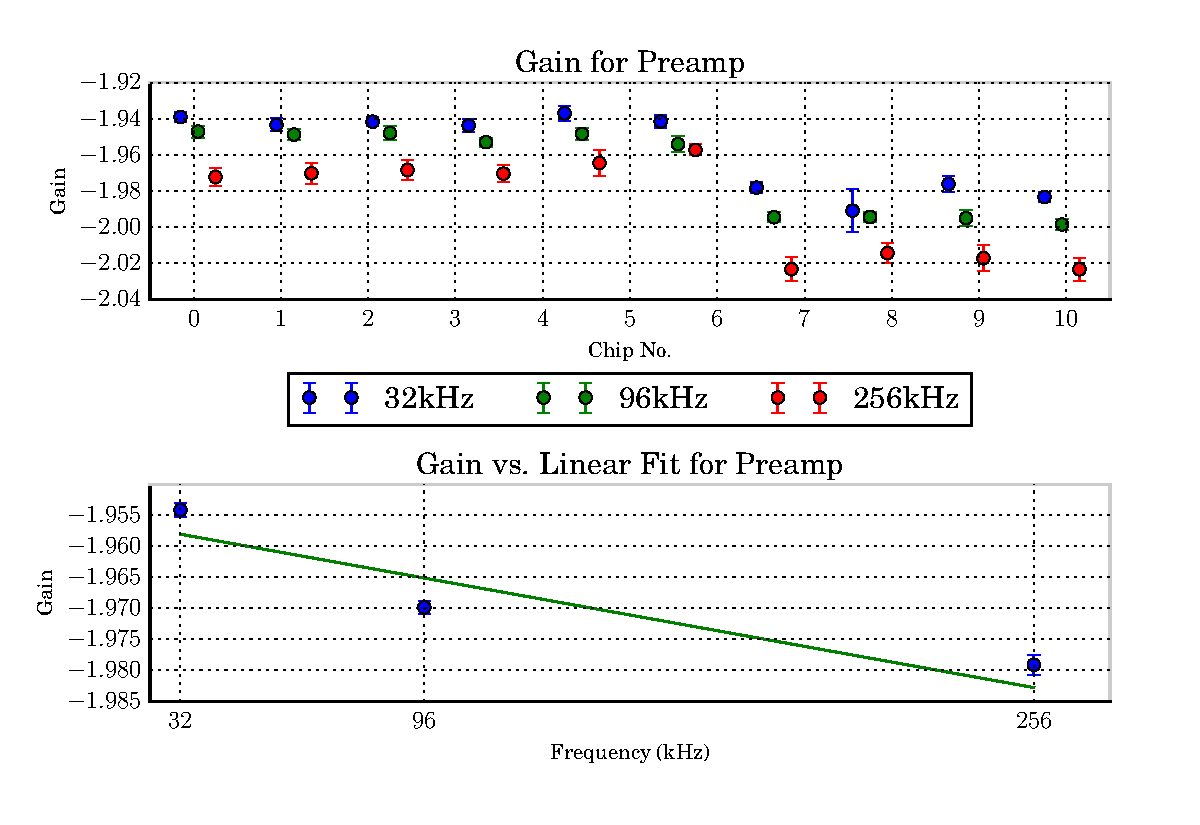
\includegraphics[width=\linewidth]{images/plots/dc_slope_preamp_gain-2.pdf}
    \caption{Effective gains of pre-amplifier at different sampling frequencies. The configured gain is -2.}
    \label{fig:preamp_slope-2}
\end{figure}
\begin{figure}
    \centering
    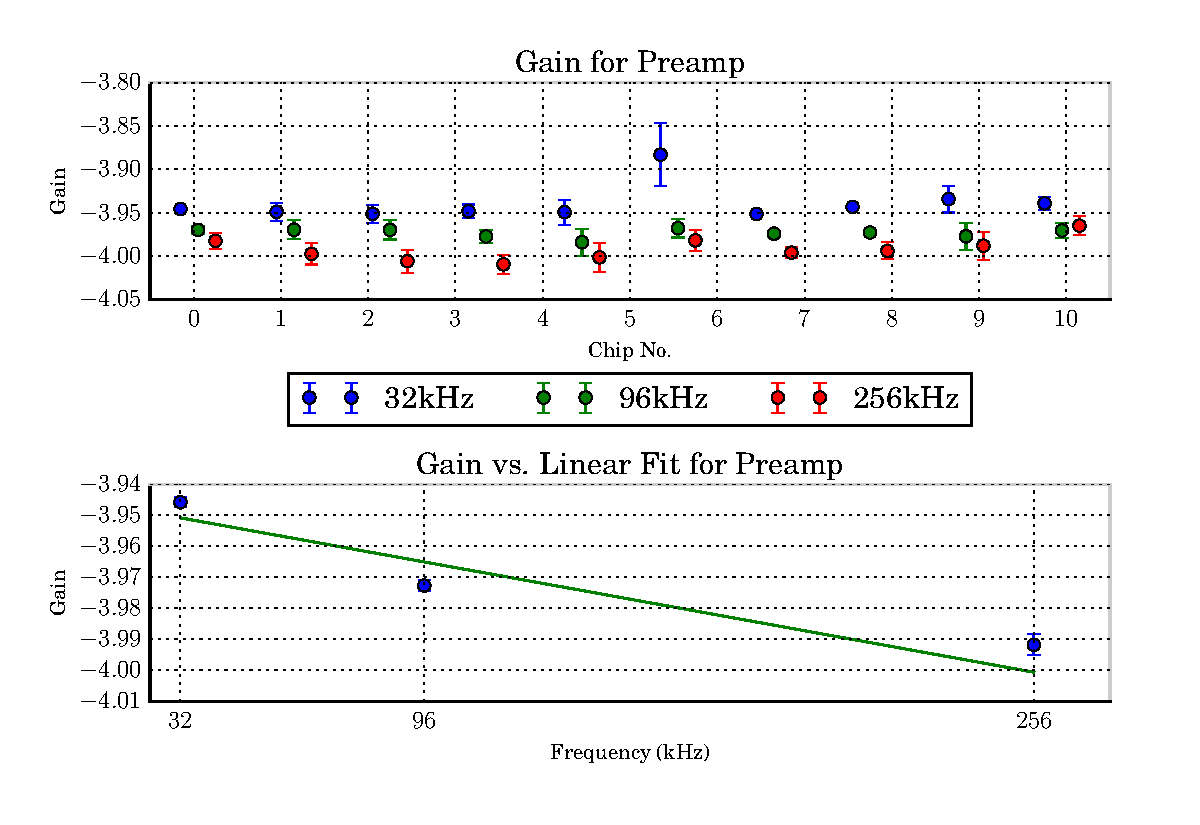
\includegraphics[width=\linewidth]{images/plots/dc_slope_preamp_gain-4.pdf}
    \caption{Effective gains of pre-amplifier at different sampling frequencies. The configured gain is -4.}
    \label{fig:preamp_slope-4}
\end{figure}
\begin{figure}
    \centering
    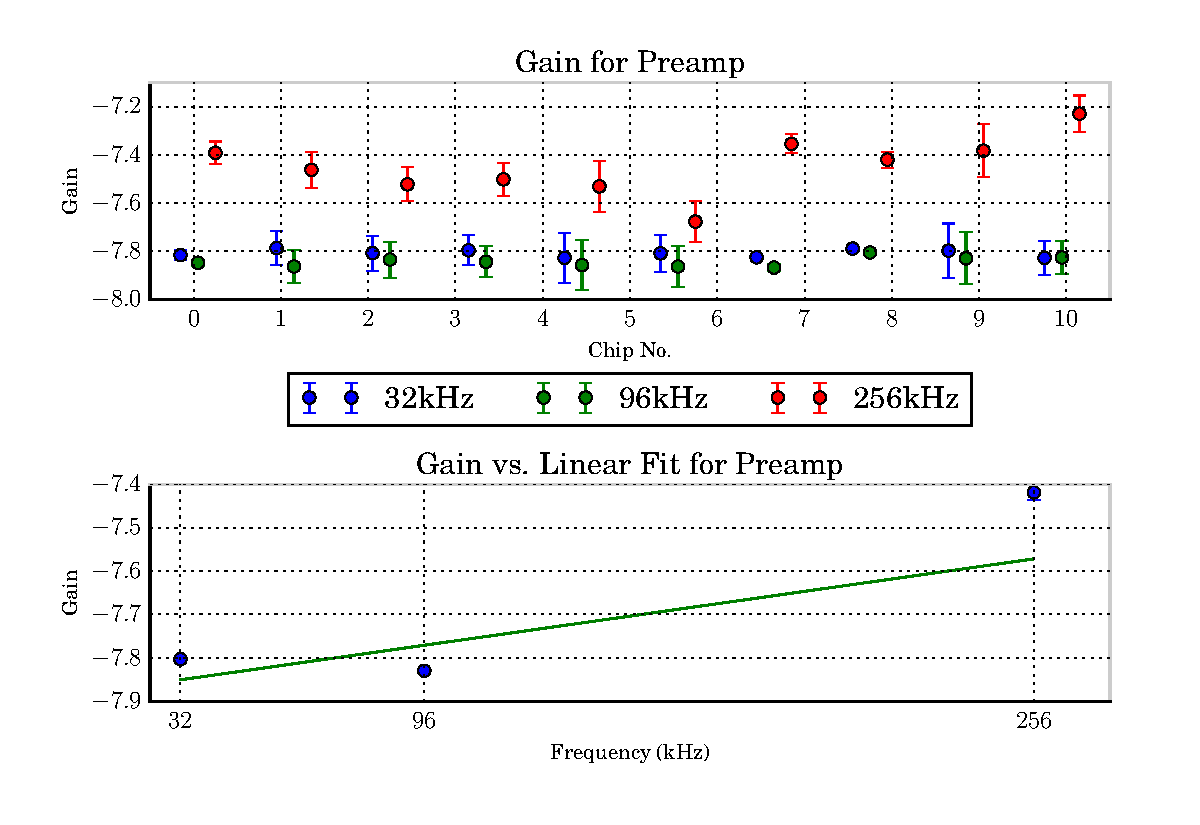
\includegraphics[width=\linewidth]{images/plots/dc_slope_preamp_gain-8.pdf}
    \caption{Effective gains of pre-amplifier at different sampling frequencies. The configured gain is -8.}
    \label{fig:preamp_slope-8}
\end{figure}
\begin{figure}
    \centering
    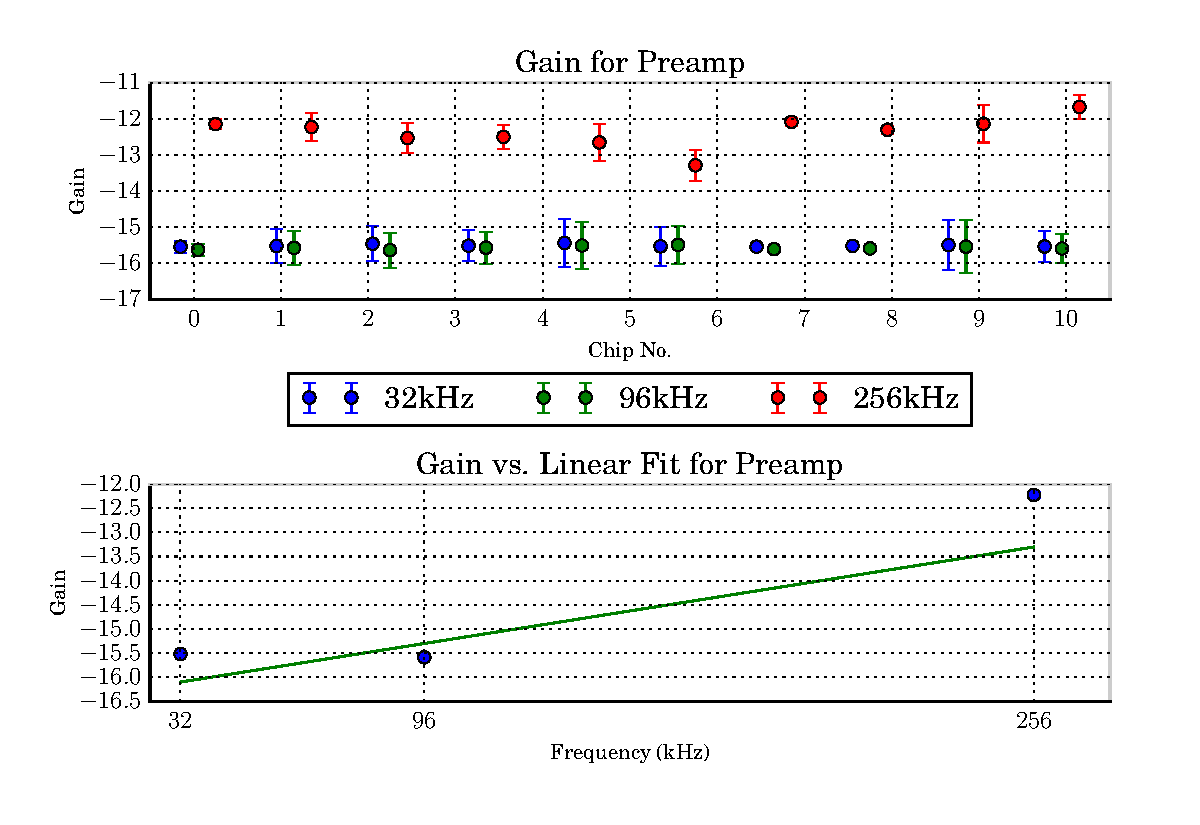
\includegraphics[width=\linewidth]{images/plots/dc_slope_preamp_gain-16.pdf}
    \caption{Effective gains of pre-amplifier at different sampling frequencies. The configured gain is -16.}
    \label{fig:preamp_slope-16}
\end{figure}

Another   interesting  figure  to  look  at  might  be  the  offset   of   the
pre-amplifier. In much the same way,  the offsets are presented in function of
gain and sampling frequency in figures

\begin{figure}
    \centering
    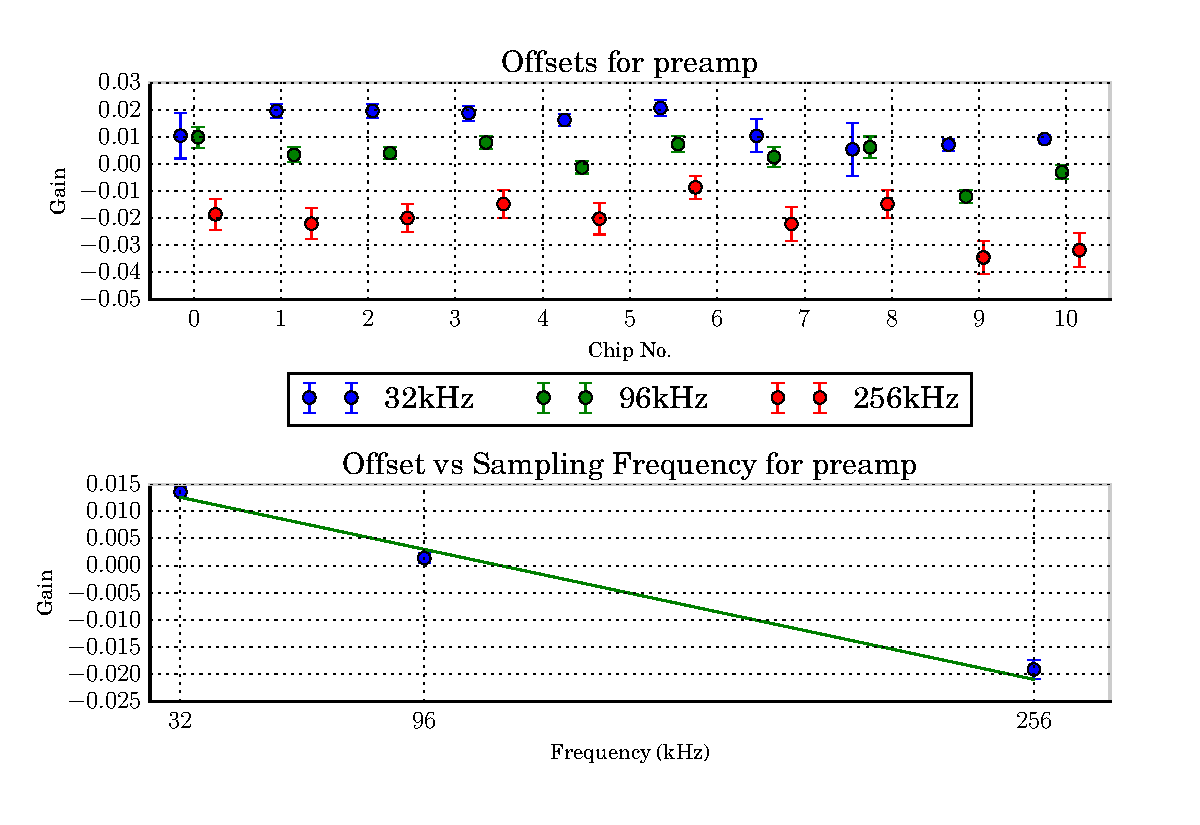
\includegraphics[width=\linewidth]{images/plots/dc_offsets_preamp.pdf}
    \caption{Effective offsets of preamp at different sampling frequencies. The configured gain is 1.}
    \label{fig:preamp_offsets}
\end{figure}

% --------------------------------------------------------------------------- %
\section{Sigma-Delta Converter: DC Measurements}
\label{sec:sigdelDC}
% --------------------------------------------------------------------------- %

The \sdm~was measured directly, isolated from the preamp, by applying a number
of  constant  DC  voltages  to  the \signal{TEST OUT} pin  and  recording  the
resulting bit streams using the GPIO \raspi.

Following  the  same  principles as with the pre-amplifier, for every chip and
for every sampling frequency, 11 different input voltages were applied and the
output bit  stream  was  recorded.  All of the data was then evaluated using a
third order sinc-decimation filter to reconstruct a  digital  version  of  the
measured voltage.

By fitting the linear function $y=mx+q$ to  the  11  input/output voltage data
points, we expect to obtain a  line  who's  incline  is  equal to 1 and offset
equal to 0. In figure \ref{fig:sigdel_gain}  each  incline  of  each  chip  is
plotted for  each  sampling frequency $fs$. Similarly, the offset of each chip
is plotted in figure \ref{fig:sigdel_offset}.

\begin{figure}
    \centering
    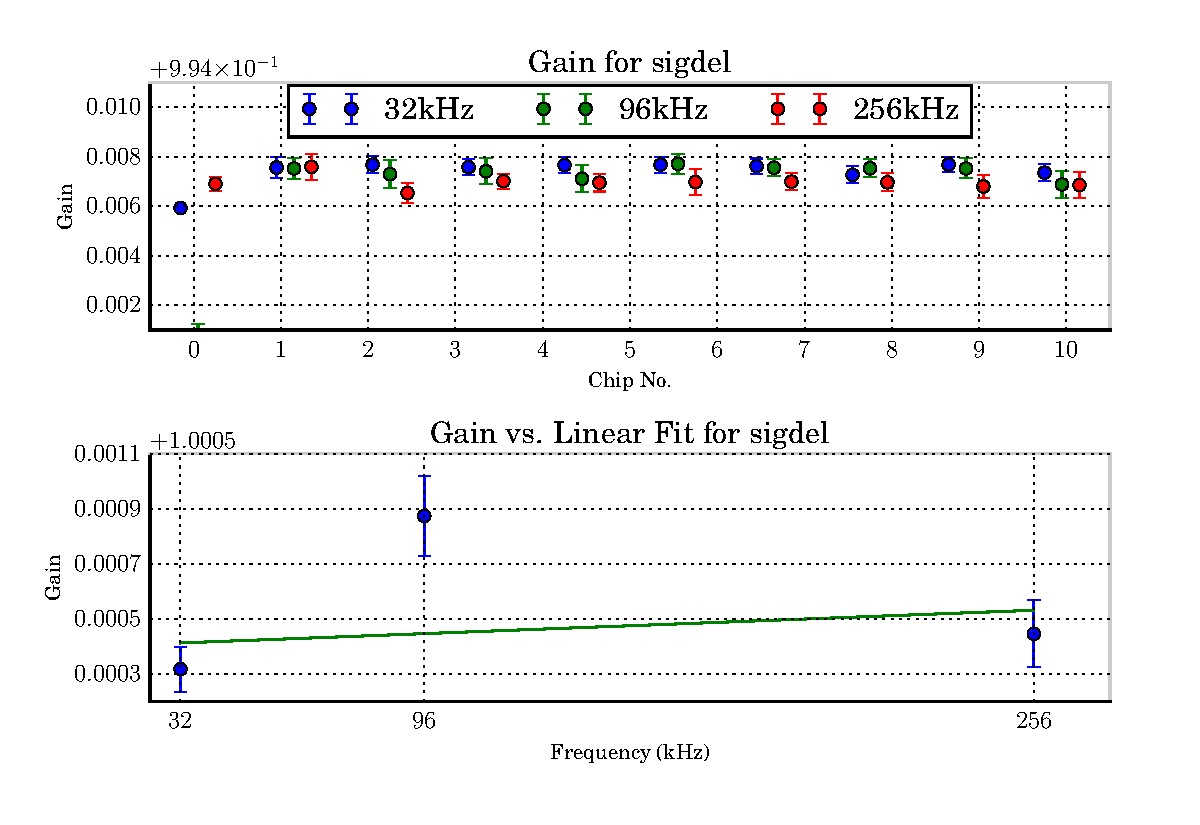
\includegraphics[width=\linewidth]{images/plots/dc_slope_for_sigdel.pdf}
    \caption{Effective gain/linearity of \sdm~at different sampling frequencies.}
    \label{fig:sigdel_gain}
\end{figure}
\begin{figure}
    \centering
    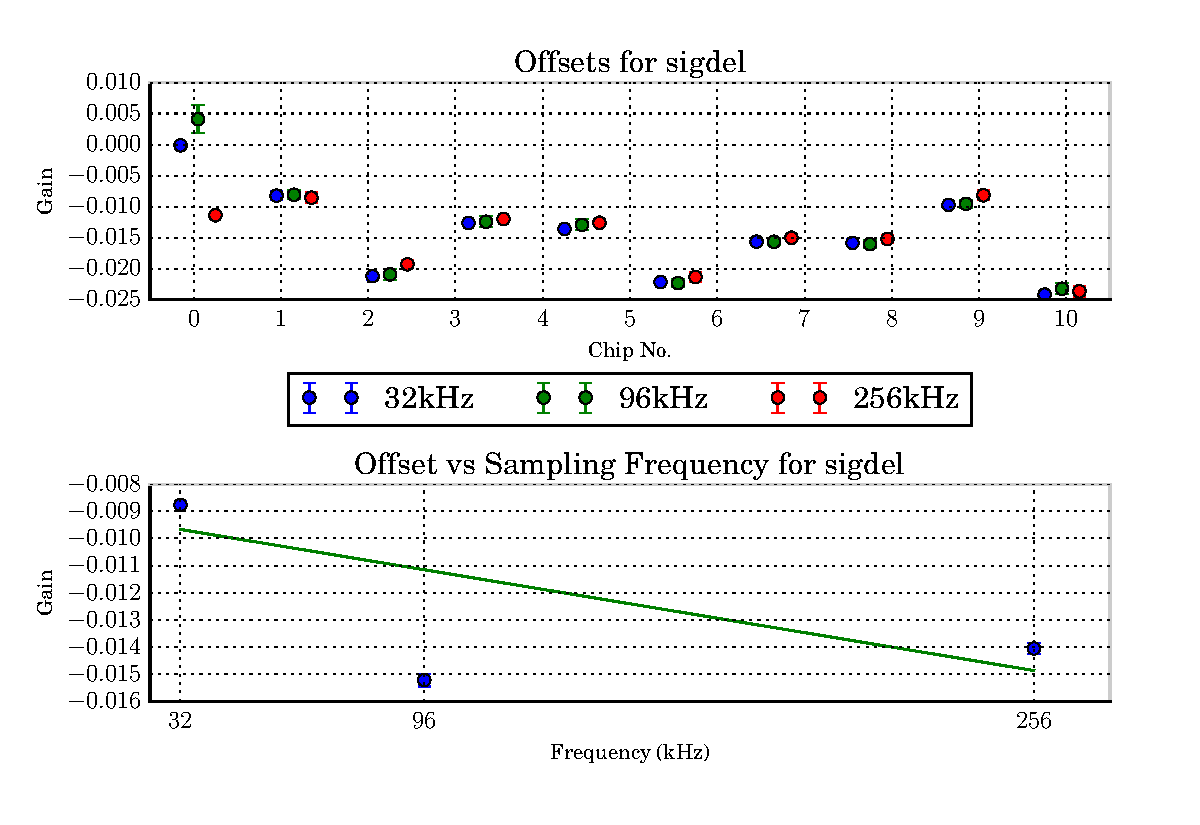
\includegraphics[width=\linewidth]{images/plots/dc_offsets_sigdel.pdf}
    \caption{Effective offset of \sdm~at different sampling frequencies.}
    \label{fig:sigdel_offset}
\end{figure}

The  results  show that there is no significant deviation  from  the  expected
values.

During processing of the bit stream data, some anomalies were noticed.  Random
spikes would  occur  here and there. See figure \ref{fig:noisy_sigdel}.

\begin{figure}
    \centering
    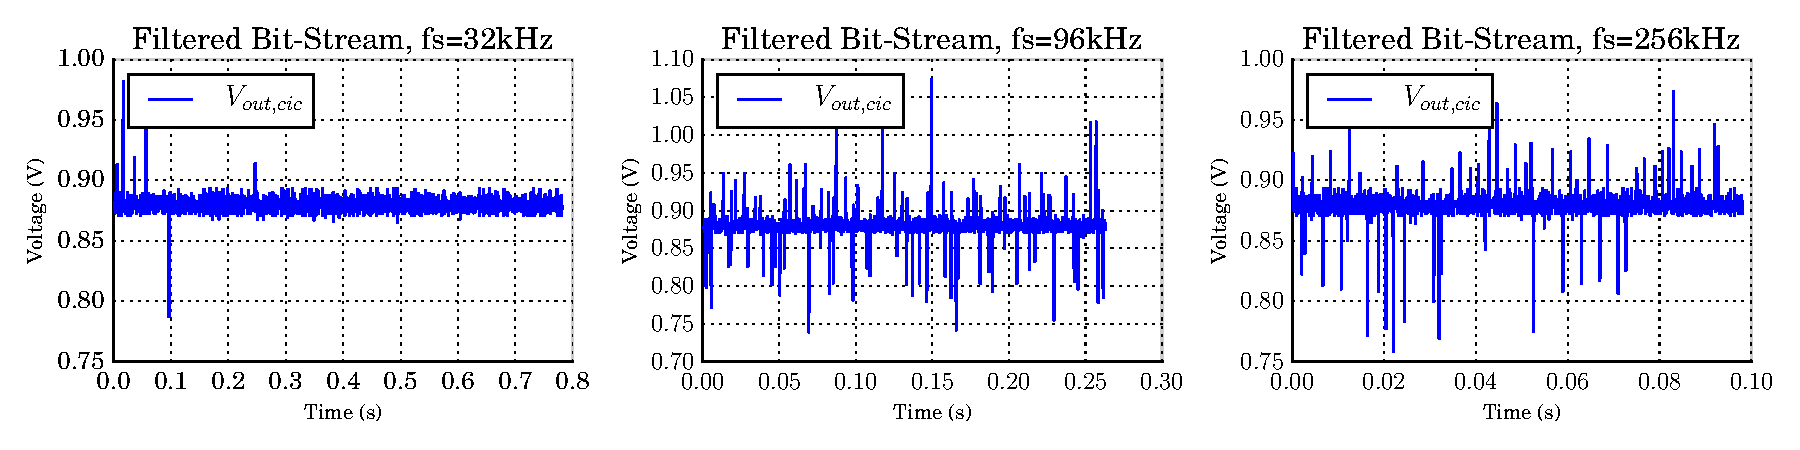
\includegraphics[width=\linewidth]{images/plots/noisy_bitstream.pdf}
    \caption{Large, random spikes after filtering the bit stream.}
    \label{fig:noisy_sigdel}
\end{figure}
.
The only correlations that could  be  made  were that the
spikes  occurred  more  often  at  higher sampling rates than they do at lower
sampling rates. After analysing the time axis  to  make  sure  the data points
were  equidistantly  spaced,  random  deviations  were  detected.  This  could
possibly   be   a  result  of  using  the  rather   inaccurate   system   call
\textit{gettimeofday()}  for  generating  time  stamps  on  the   \raspi.  The
deviations are large enough to  suggest the possibility that bits went missing
from the bit stream.

% --------------------------------------------------------------------------- %
\section{Complete System: DC Measurements}
\label{sec:systemDC}
% --------------------------------------------------------------------------- %

The  same  measurements  were  performed  on  the complete chip: That is,  the
pre-amplifier and the \sdm~were measured together as one.

As expected, the rather imperfect results from the pre-amplifier combined with
the perfect results from the \sdm~result in a  semi-imperfect  system. Figures
\ref{fig:both_gain}  and  \ref{fig:both_offset}  show  the  various gains  and
offsets of the complete system.

\begin{figure}
    \centering
    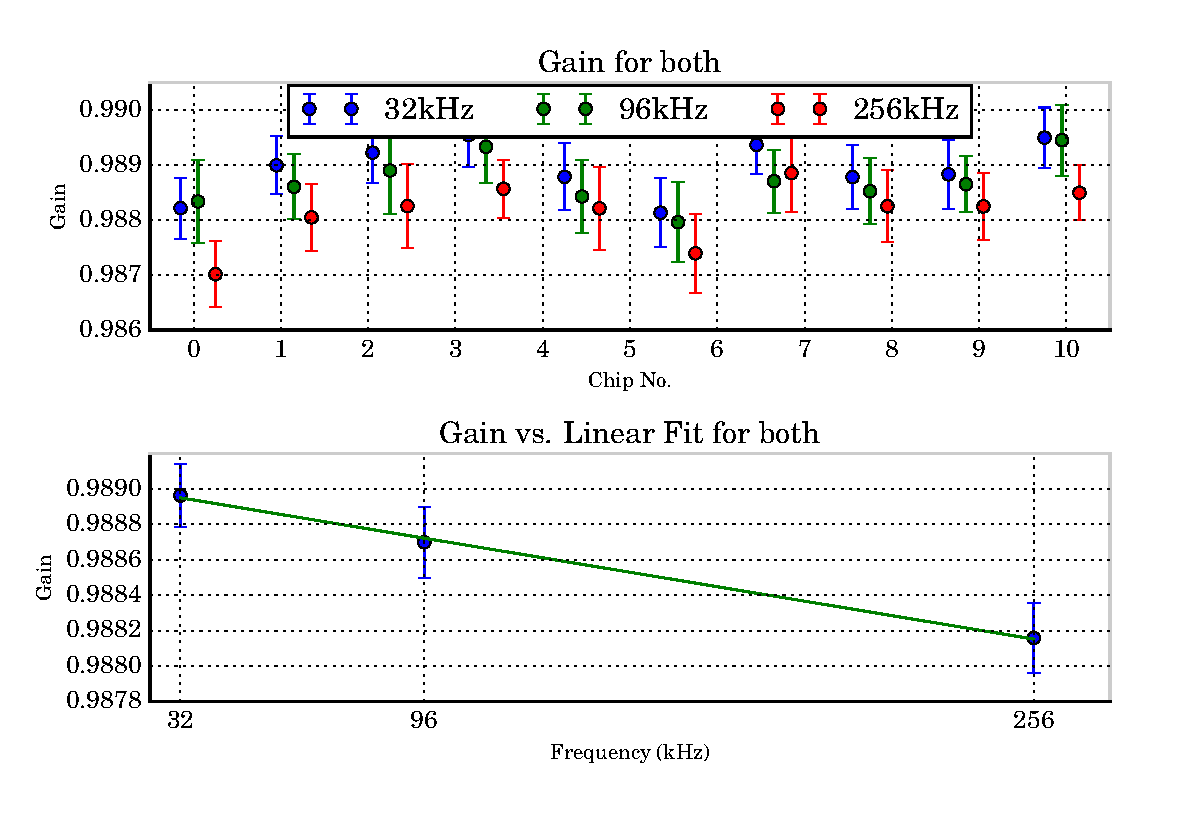
\includegraphics[width=\linewidth]{images/plots/dc_slope_for_both.pdf}
    \caption{Effective gain of the whole system at different sampling frequencies. The configured gain is 1.}
    \label{fig:both_gain}
\end{figure}
\begin{figure}
    \centering
    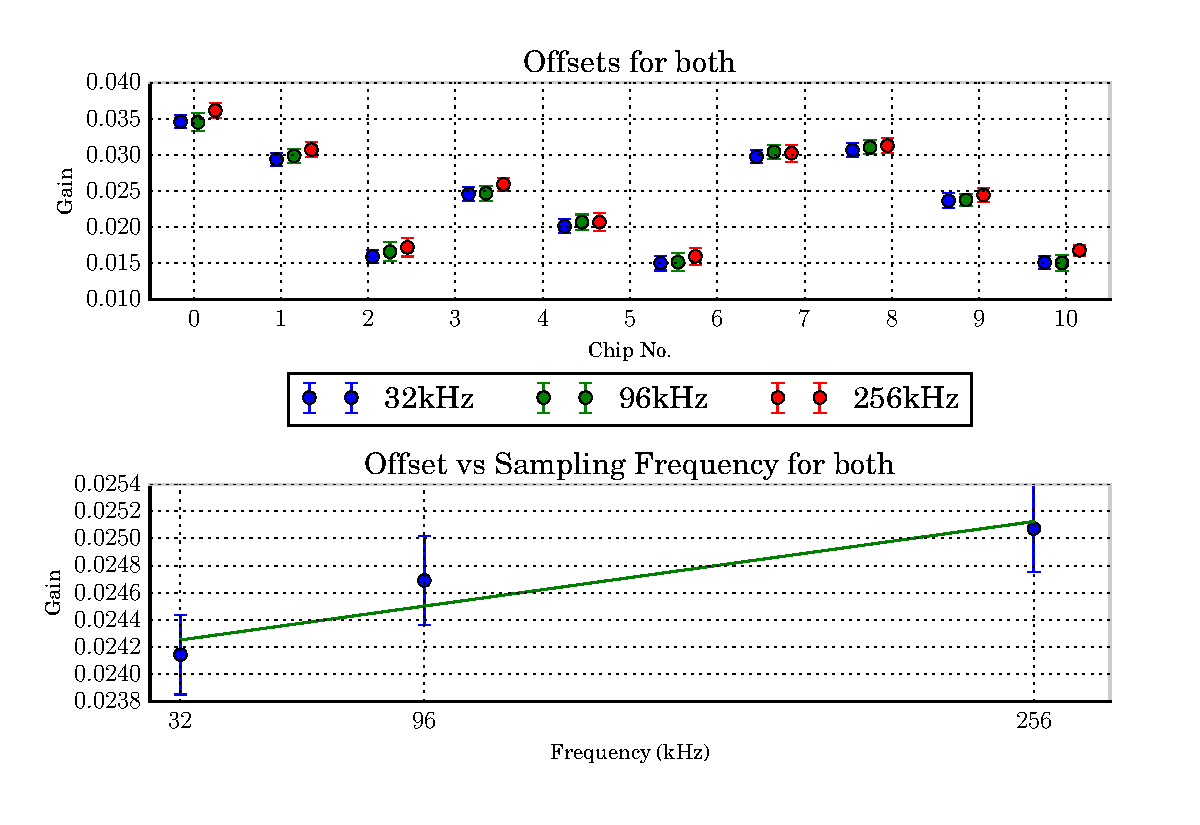
\includegraphics[width=\linewidth]{images/plots/dc_offsets_both.pdf}
    \caption{Effective offset of the whole system at different sampling frequencies. The configured gain is 1.}
    \label{fig:both_offset}
\end{figure}

% ---------------------------------------------------------------------------- %
\chapter{Conclusions and Outlook}
\label{chap:conclusions}
% ---------------------------------------------------------------------------- %

This project's  main objectives  were to create  and document  a comprehensive
test bench  and the corresponding  data processing  tools, and to  measure and
assess  the performance  and  characteristics of  the  \sdm.  Originally,  the
plan  was  to  to  measure  new  chip  designs  which  build  upon  the  first
iteration. However, as  we found out during  the project, the new  chips would
not arrive in  time to perform these measurements. Therefore, we  fell back to
the original chip design in our measurements.

Developing the test  bench  and  the  data processing tools turned out to be a
noticeably more  complex undertaking than originally anticipated, and progress
was not as swift as we had hoped.  Additionally,  some time was lost due to an
incorrect component having been soldered onto  the  test board, requiring time
for finding and fixing the error. Lastly, we  occasionally  got hung up on the
wrong  details,  investing  time  without  generating   much   usable  output.

This resulted  in  some  delays,  which  means  not  all  objectives have been
achieved  at  this point. Specifically, mapping the measurement results to the
internal  architecture  of  the  chip  via simulations still needs to be done.
However, the test bench and data processing tools  have  been  developed  to a
satisfying and  very  usable  state,  allowing  for  quick  measurement  of  a
multitude of chips and analysis of the resulting data.

As  was  already established in the previous  work\cite{ref:gloor},  the  poor
characteristics  of  the pre-amplifier  are  the  main  cause  for  diminished
performance  of  the  device.  In  this  work,  measurements  have  shown  the
pre-amplifier having a  rather  large  offset  and a gain that varies strongly
depending  on  the operating frequency. Deviations in effective  gain  can  be
traced back to slow rise and  fall  times  of the switched capacitor OTA; When
the operating  frequency  is  close to the limit (which turns out to be around
\SI{256}{\kilo\hertz}), the  target output voltage of the pre-amplifier can no
longer  be  reached within one clock cycle and the  converted  value  deviates
strongly as a result.

There  are  multiple possible reasons for the slow rise and  fall  times.  The
transconductance of the OTA might  be  too  low. Increasing it leads to better
performance,  but  at  the  cost  of  higher power consumption. Decreasing the
values of the switched capacitors can lead to faster rise and fall times,  but
at the cost of higher noise and more susceptibility to parasitic capacitances.
Considering   the   fact   that   the   switched   capacitors   are   in   the
\SI{100}{\femto\farad}-range, and considering  the fact that the output of the
pre-amplifier is directly connected  to a lead on the chip (which is typically
in  the  \SI{}{\pico\farad}-range),  the  lead  may  very  well  have a strong
negative influence  on  the  pre-amplifier's  performance.  This  hasn't  been
tested, but may be worth considering.

Without the aid of simulations, we can't make more decisive conclusions.

On the bright side, though, the \sdm~appears to perform quite well.

- objective: develop test bench and data processing stuff
- success: moderately: test bench ok, scripts okay-ish, no simulations
- why not? time delays
- how to proceed into p6?


\begin{itemize}\tightlist
    \item
        Short recap: What did we want to achieve?
    \item
        Were we successful?
    \item
        If not: Why? How do we proceed from here?
    \item
        How to proceed from here into P6?
\end{itemize}


% -------------------------------------------------------- %
% Bibliography: We  are using  the  IEEEtran package  from %
% Michael Shell                                            %
%                                                          %
% There  are  a  few  different  styles  in  the  IEEEtran %
% package.   We are  going to  use  one of  two of  those, %
% either in the sorted or unsorted variety.                %
%                                                          %
% The sorted  version sorts  bibliographic entries  in the %
% bibliography alphabetically, while  the unsorted version %
% lists bibliographic  entries in the order  in which they %
% were cited (first occurrence).                           %
% -------------------------------------------------------- %
%\bibliographystyle{bibliography/IEEEtranS} % sorted
%\raggedright
\bibliographystyle{bibliography/IEEEtran} % unsorted
\bibintoc
\bibliography{bibliography/references}
\todo[inline]{%
    Make sure to have the right IEEE style and all that good stuff
}

% -------------------------------------------------------- %
% Appendices are  usually numbered  and therefore  part of %
% the mainmatter, not the backmatter.                      %
% The advice about meaningful chapter names applies to the %
% appendices as well, see above.                           %
% -------------------------------------------------------- %
\appendixpage
\appendix
%% ---------------------------------------------------------------------------- %
\chapter{Configuration of Laboratory Equipment}
\label{chap:labconfig}
% ---------------------------------------------------------------------------- %

This chapter contains supplementary information for configuring the laboratory
equipment used during the project.

% ---------------------------------------------------------------------------- %
\section{HP Arbitrary Waveform Generator}
\label{sec:HPwave}
% ---------------------------------------------------------------------------- %

Configuring the waveform generator consists of two primary parts:

\begin{itemize}\tightlist
    \item
        Making an initial configuration and storing it for later reuse.
    \item
        Restoring that configuration after a power-down event.
\end{itemize}

% ---------------------------------------------------------------------------- %
\subsection{Initial Configuration}
\label{subsec:HPwave:initialConfig}
% ---------------------------------------------------------------------------- %

When   powered  on,   the   user  will   be  greeted   by   the  screen   from
\fref{fig:HPwave:poweron}. The  first  thing  to  do  is  to  set  the  output
impedance  to  \emph{HIGH}  instead  of  \SI{50}{\ohm}. For  this,  enter  the
menu  by  pressing  \emph{Shift}  and \emph{Enter}. Then  scroll  through  the
menu  using the  \emph{>}  button until  encountering  menu item  \emph{D: SYS
MENU},  seen in  \fref{fig:HPwave:sysMenu}. Enter  the  system config  submenu
by  pressing  the  \emph{v}  key. Press   the  same  key  again  for  entering
the  \emph{OUT TERM}  submenu,  as  seen in  \fref{fig:HPwave:outTerm}. Switch
from   \emph{\SI{50}{\ohm}}   (\fref{fig:HPwave:50Ohm})   to   \emph{HIGH   Z}
(\fref{fig:HPwave:highZ}), confirm with the \emph{Enter} key.

Next,  ensure  that   a  square  wave  is  output  (default   is  sine  wave),
configure  the   frequency  to  the  desired   value  (\fref{fig:HPwave:freq},
\SI{256}{\kilo\hertz}   used   in  this   example),   set   the  VPP   voltage
to   \SI{3}{\volt}  (\fref{fig:HPwave:vpp}),   and   offset   the  signal   by
\SI{1.5}{\volt}  (the  system  expects  an  input  between  \SI{0}{\volt}  and
\SI{3}{\volt},  not   \SI{-1.5}{\volt}  and  \SI{+1.5}{\volt}),  as   seen  in
\fref{fig:HPwave:offset}.

Lastly, store  the configuration in  one of the  available slots, as  shown in
\fref{fig:HPwave:store}. This ensures  that this entire process  does not have
to be repeated after each shutdown of the device.

\todo[inline,color=purple!20!white]{%
    Would it  make sense to  arrange the images in  this section more  in line
    with  the text,  given that  this is  more of  a userguide  rather than  a
    scientific document?
}

\begin{figure}
    \centering
    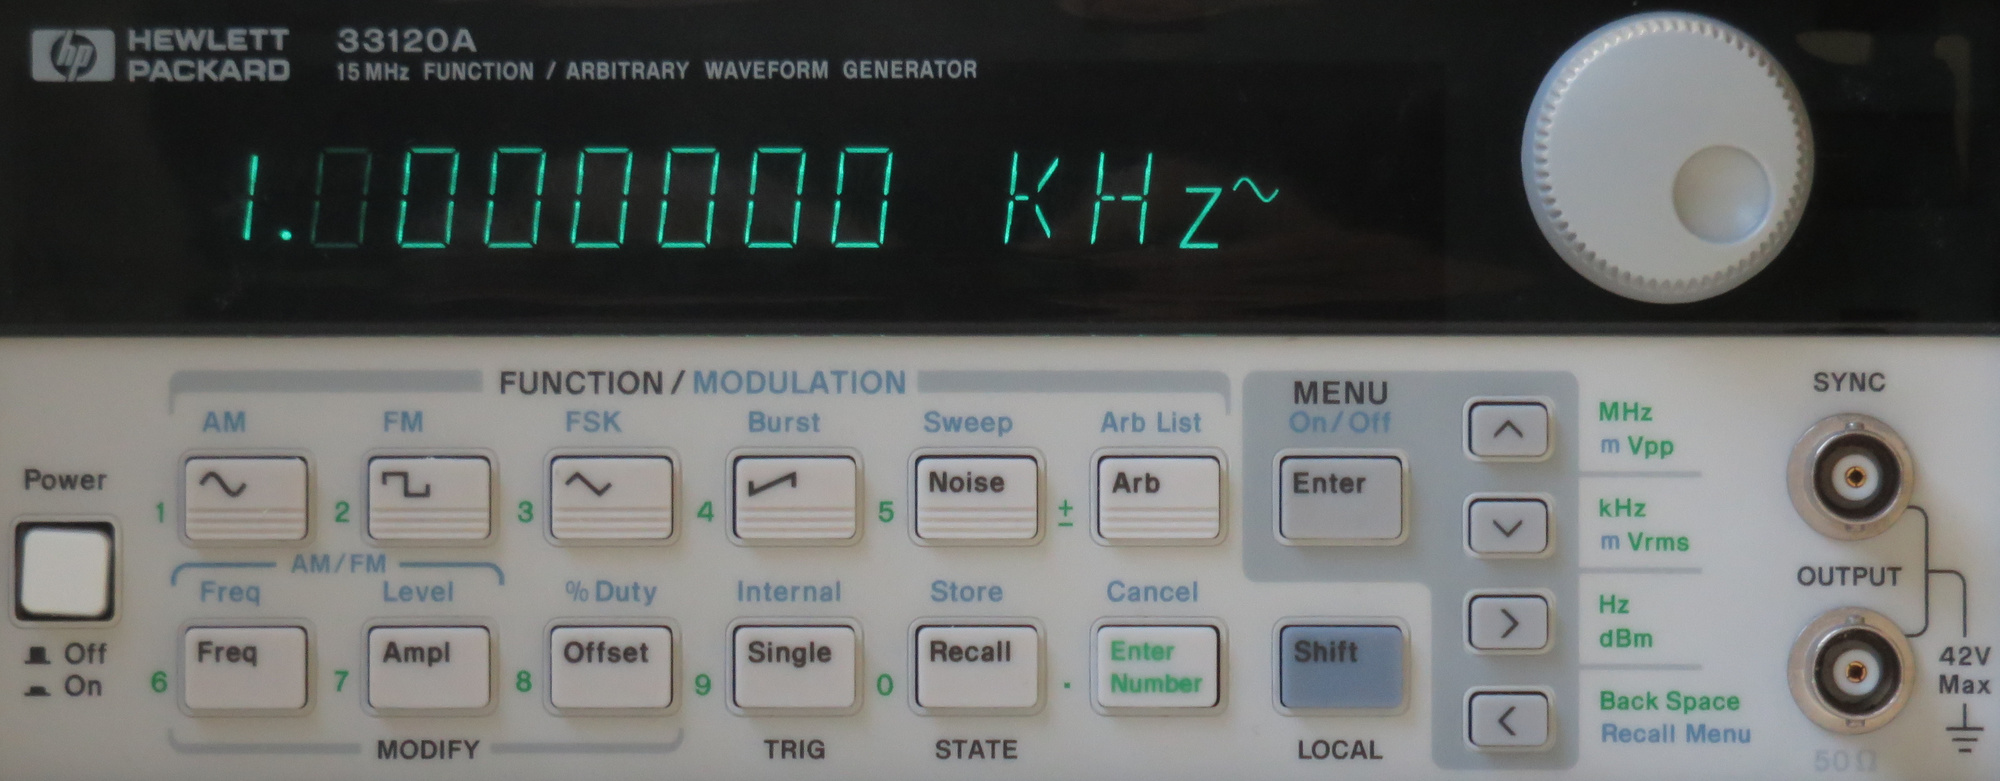
\includegraphics[width=0.67\textwidth]{images/funcGen/funcGen-01.jpg}
    \caption{Initial screen after power-on}
    \label{fig:HPwave:poweron}
\end{figure}

\begin{figure}
    \centering
    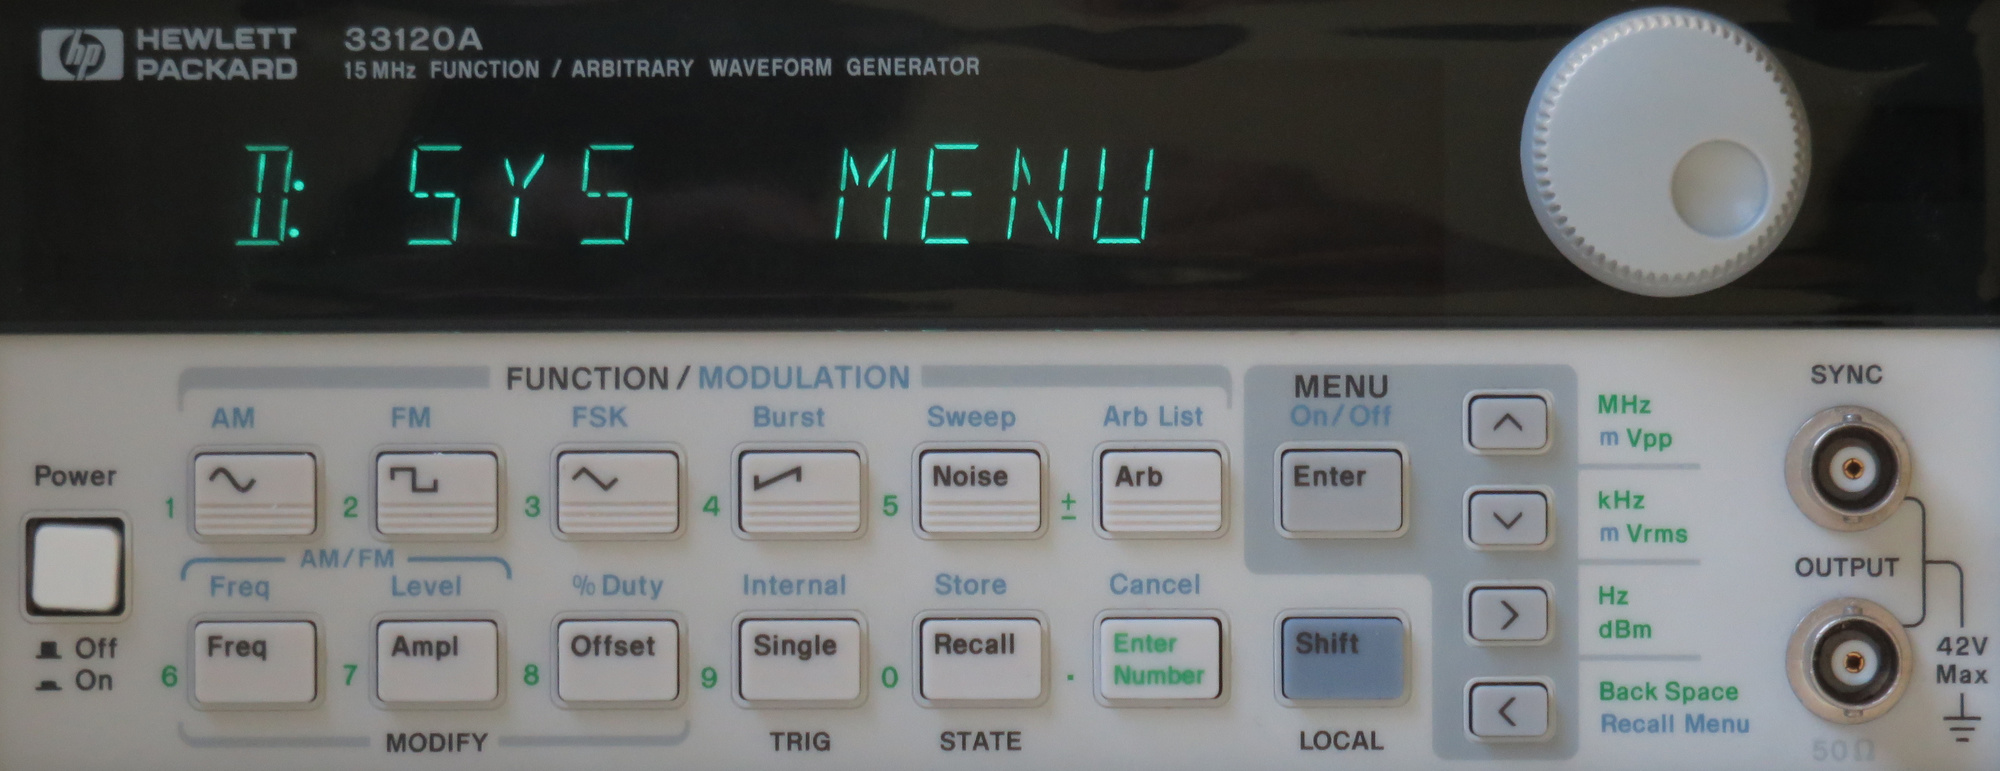
\includegraphics[width=0.67\textwidth]{images/funcGen/funcGen-02.jpg}
    \caption{System config menu}
    \label{fig:HPwave:sysMenu}
\end{figure}

\begin{figure}
    \centering
    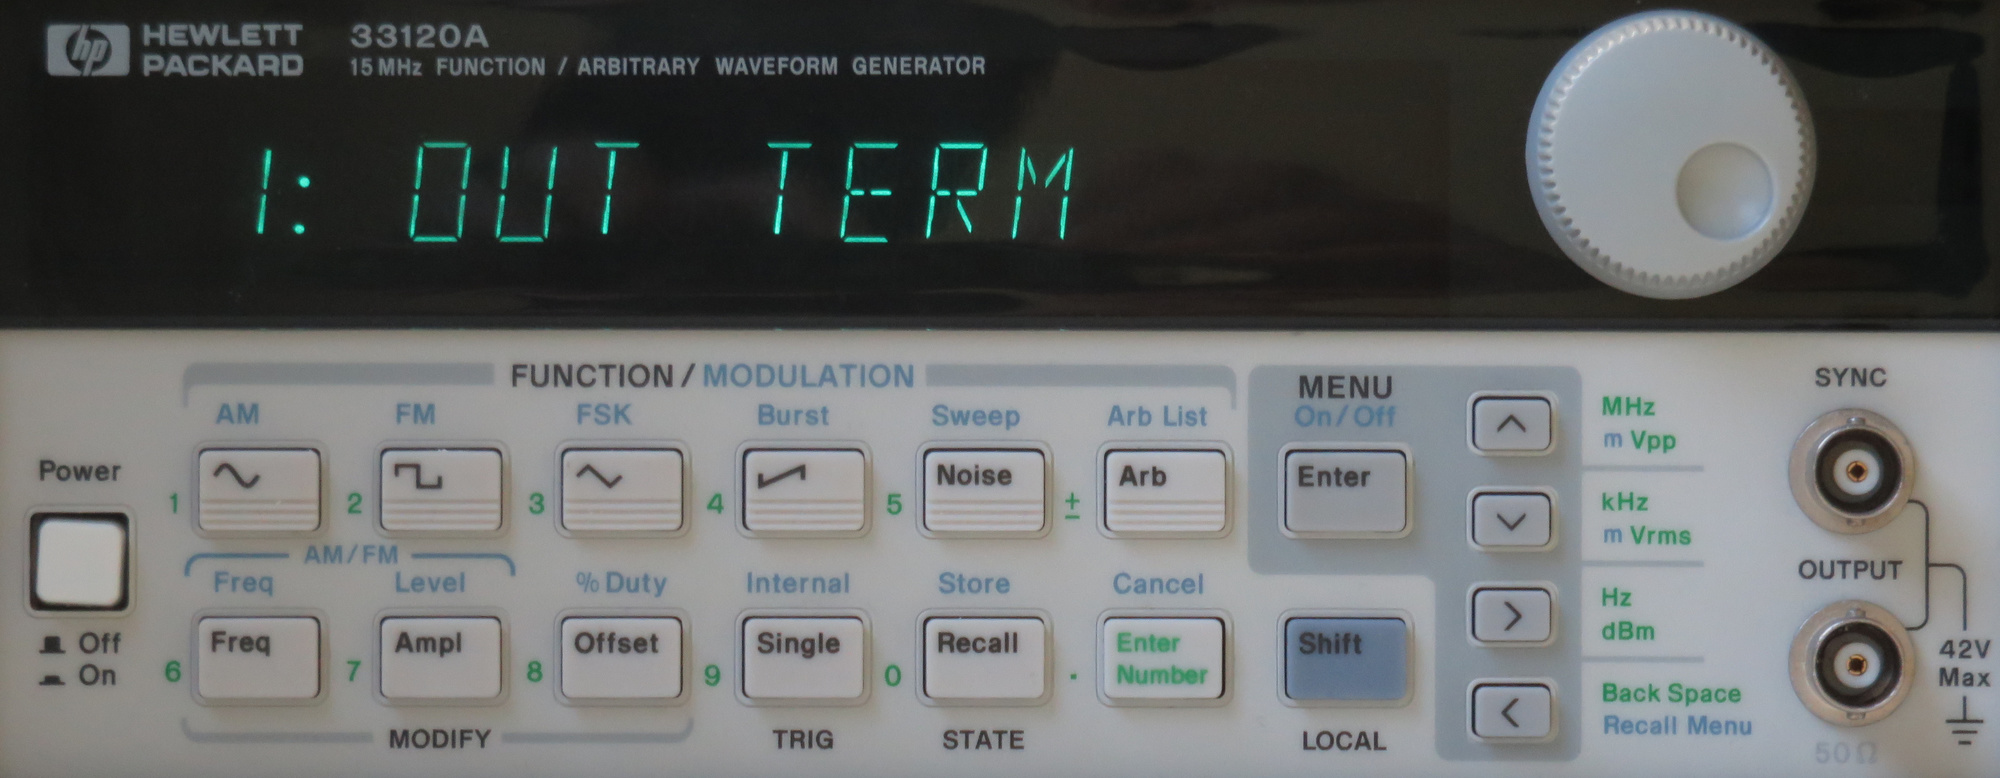
\includegraphics[width=0.67\textwidth]{images/funcGen/funcGen-03.jpg}
    \caption{Select the \emph{OUT TERM} menu item.}
    \label{fig:HPwave:outTerm}
\end{figure}

\begin{figure}
    \centering
    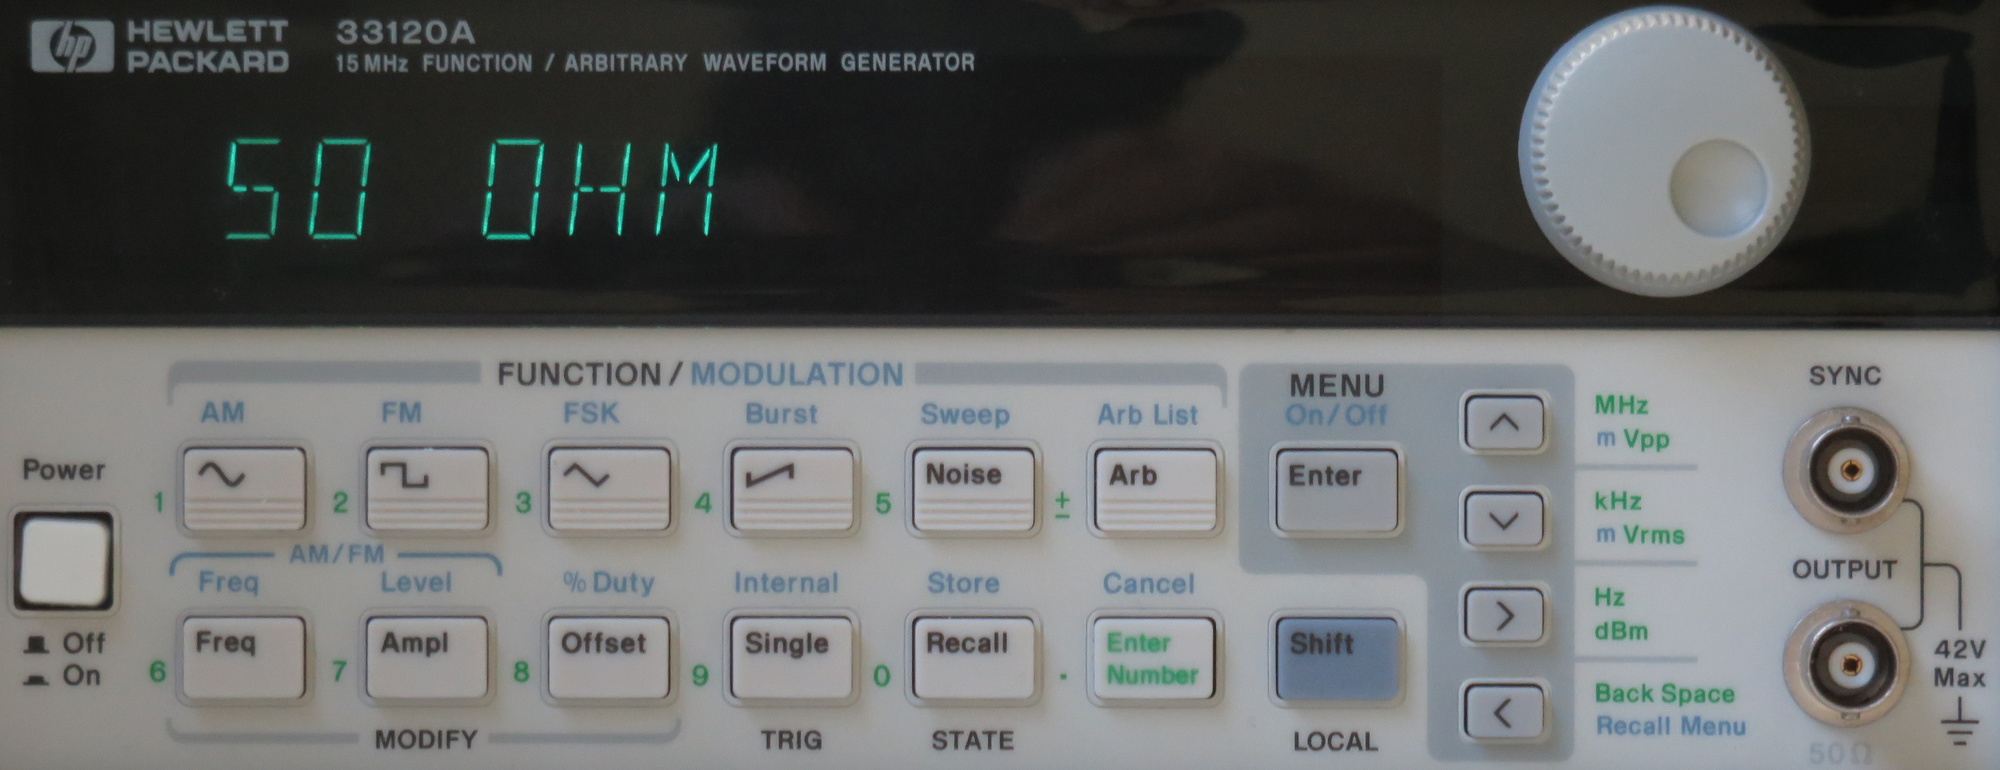
\includegraphics[width=0.67\textwidth]{images/funcGen/funcGen-04.jpg}
    \caption{By default, the output impedance is set to \SI{50}{\ohm}}
    \label{fig:HPwave:50Ohm}
\end{figure}

\begin{figure}
    \centering
    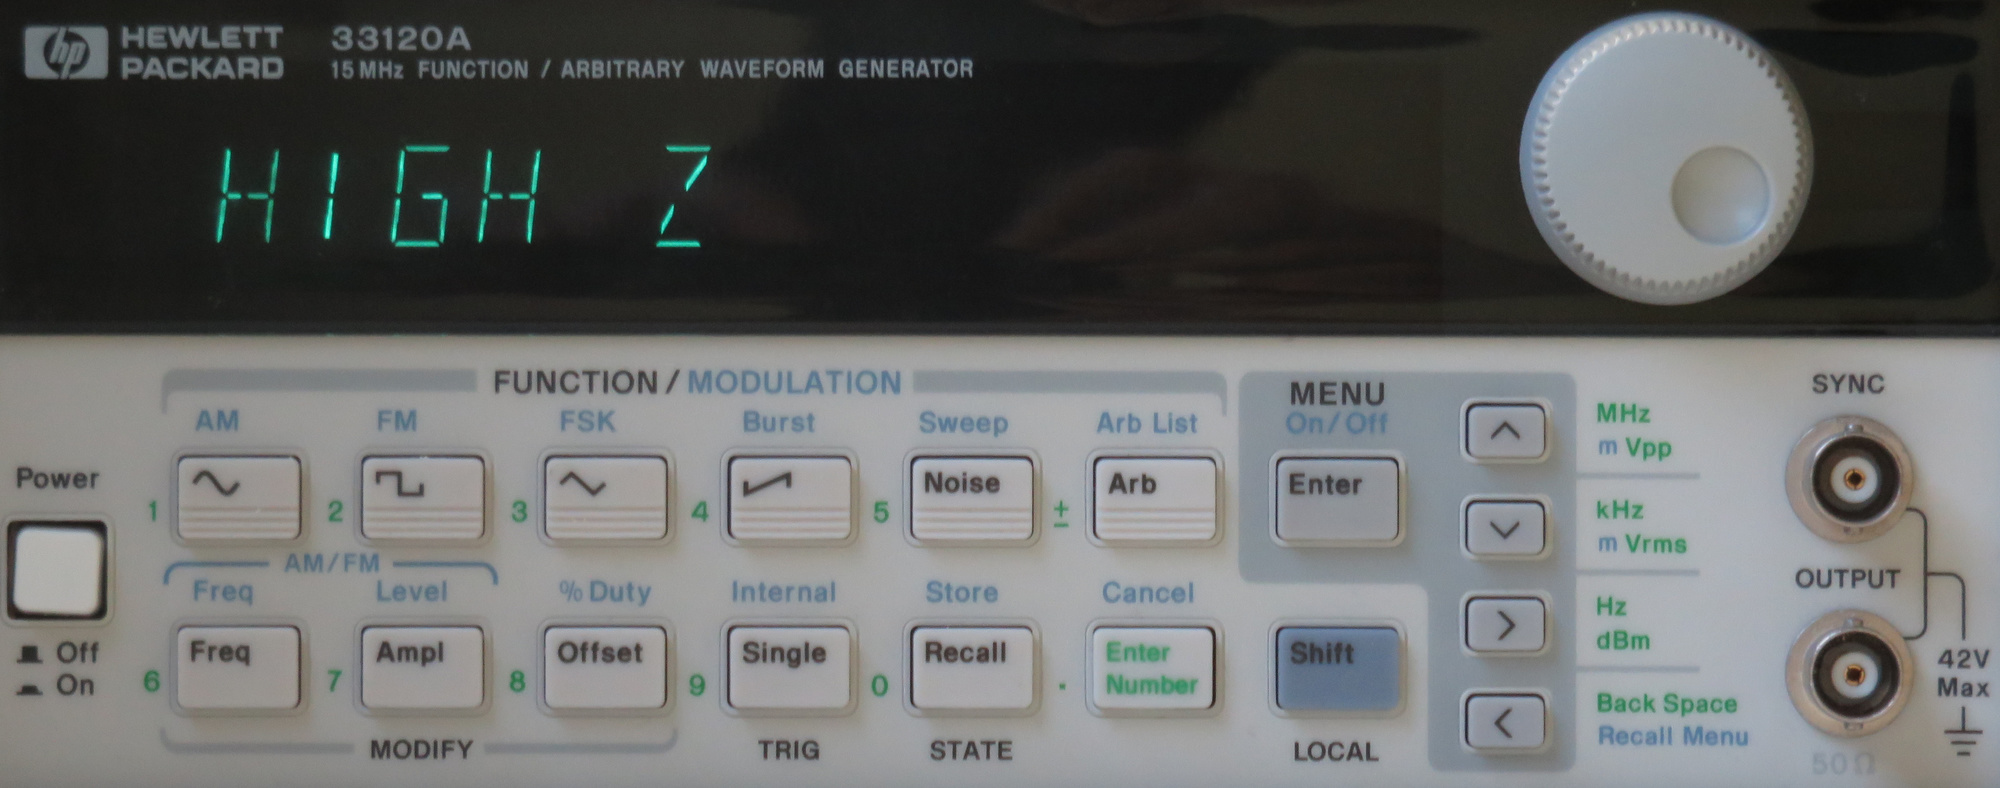
\includegraphics[width=0.67\textwidth]{images/funcGen/funcGen-05.jpg}
    \caption{Setting the output impedance to high}
    \label{fig:HPwave:highZ}
\end{figure}

\begin{figure}
    \centering
    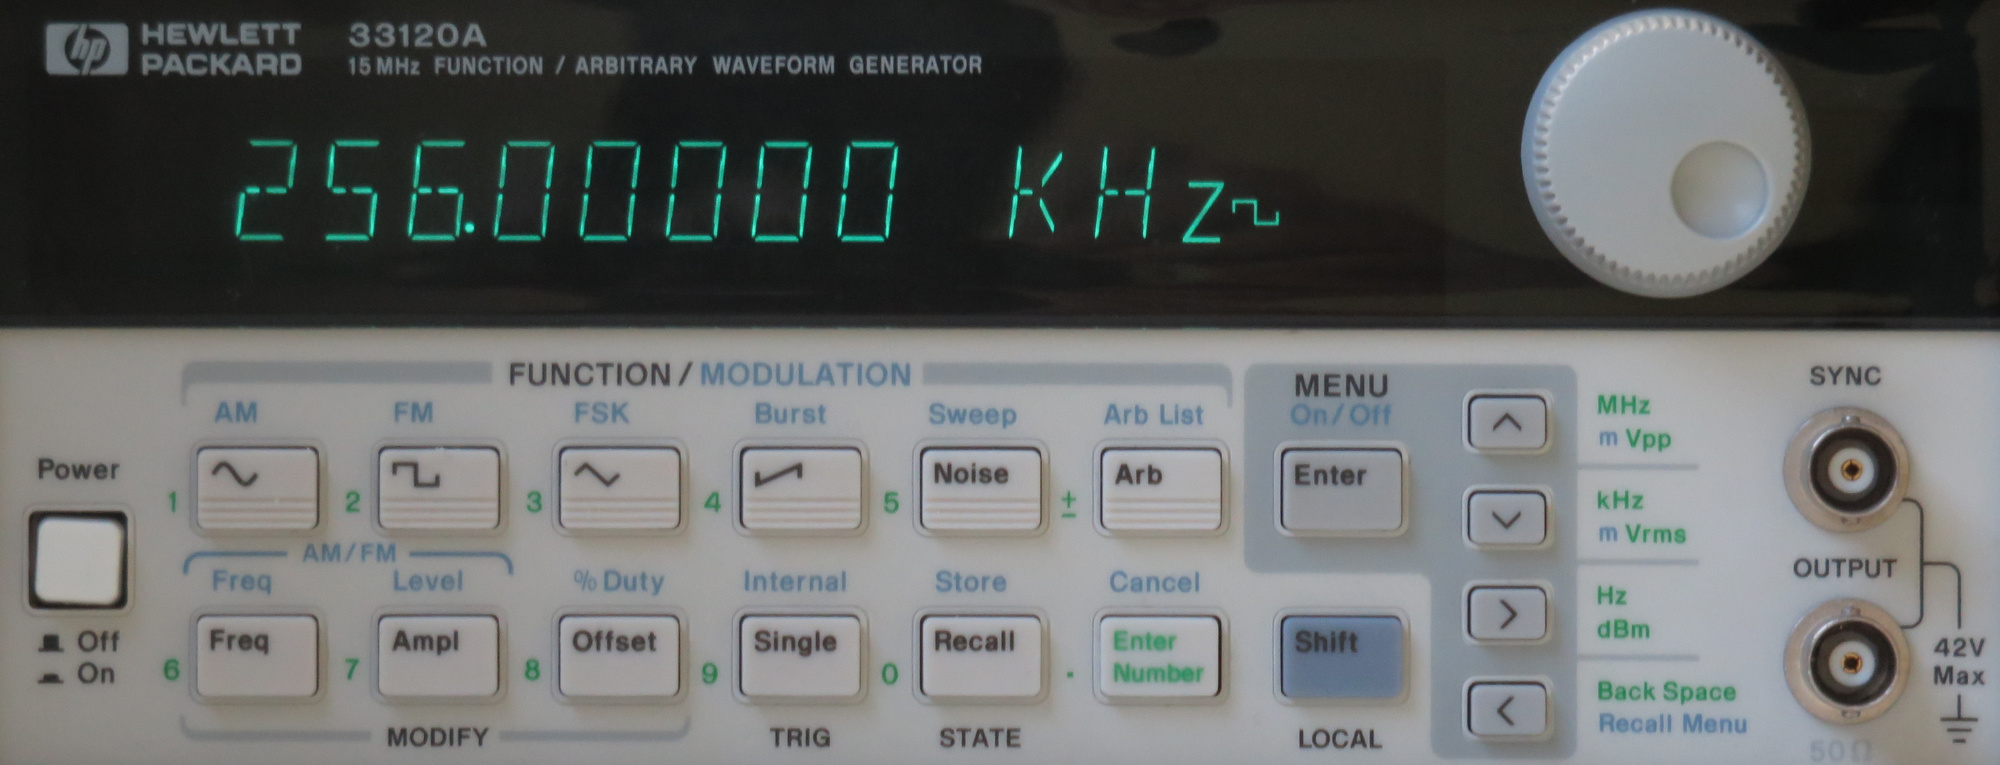
\includegraphics[width=0.67\textwidth]{images/funcGen/funcGen-06.jpg}
    \caption{Frequency configuration screen}
    \label{fig:HPwave:freq}
\end{figure}

\begin{figure}
    \centering
    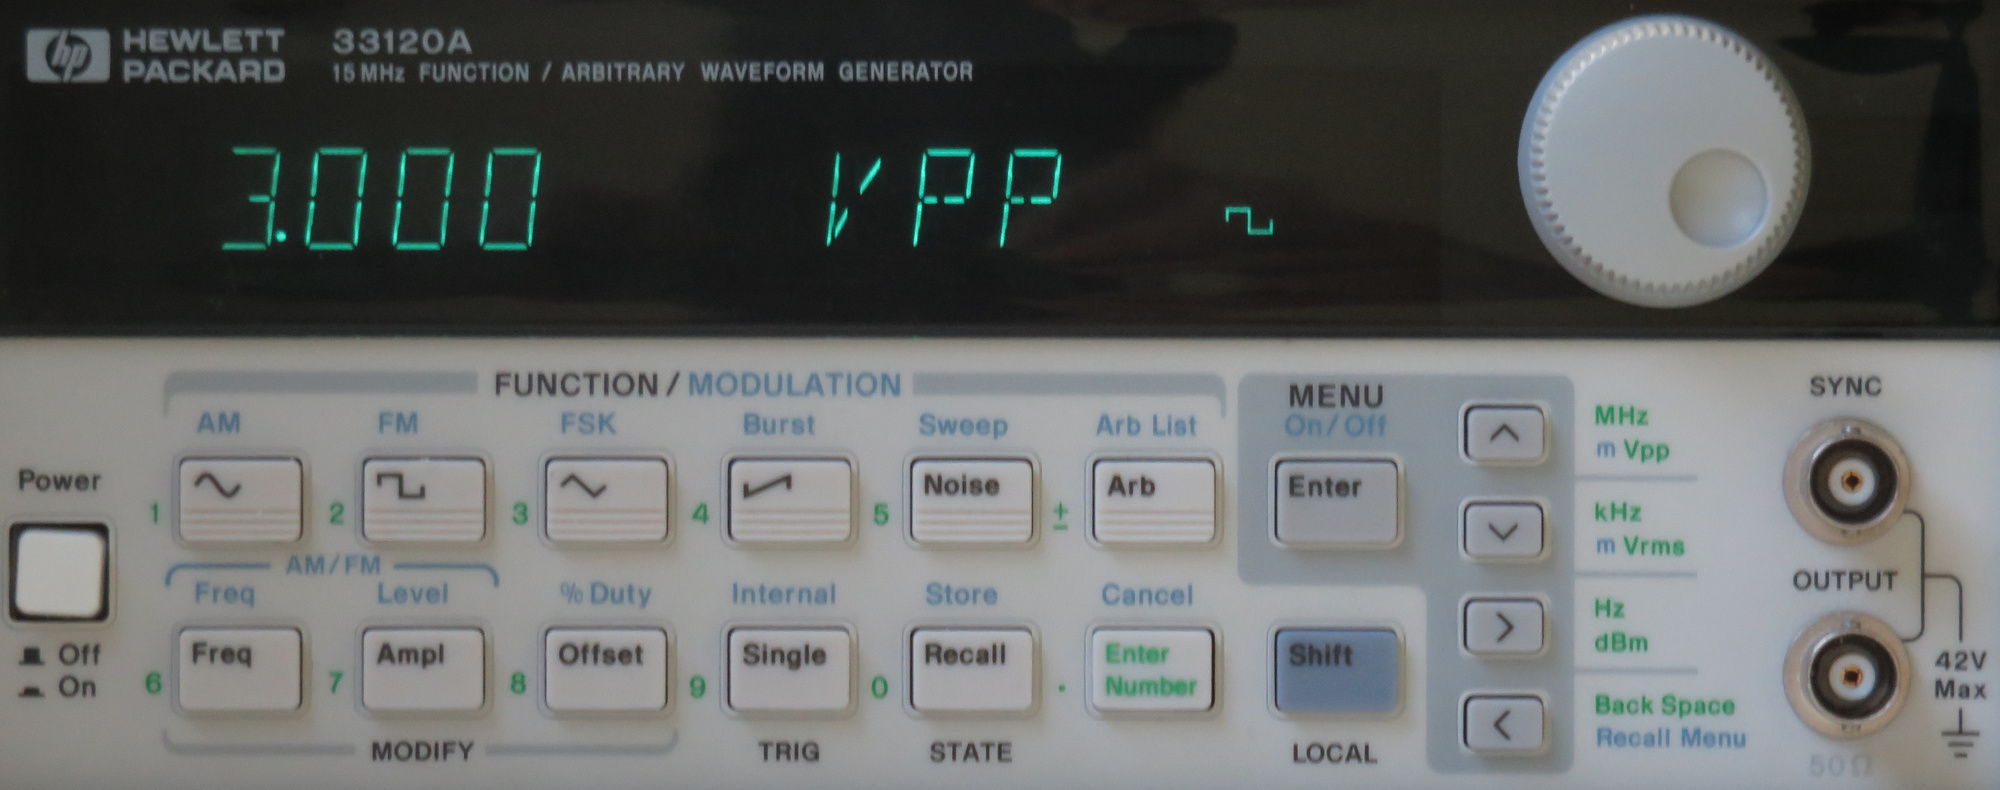
\includegraphics[width=0.67\textwidth]{images/funcGen/funcGen-07.jpg}
    \caption{VPP configuration}
    \label{fig:HPwave:vpp}
\end{figure}

\begin{figure}
    \centering
    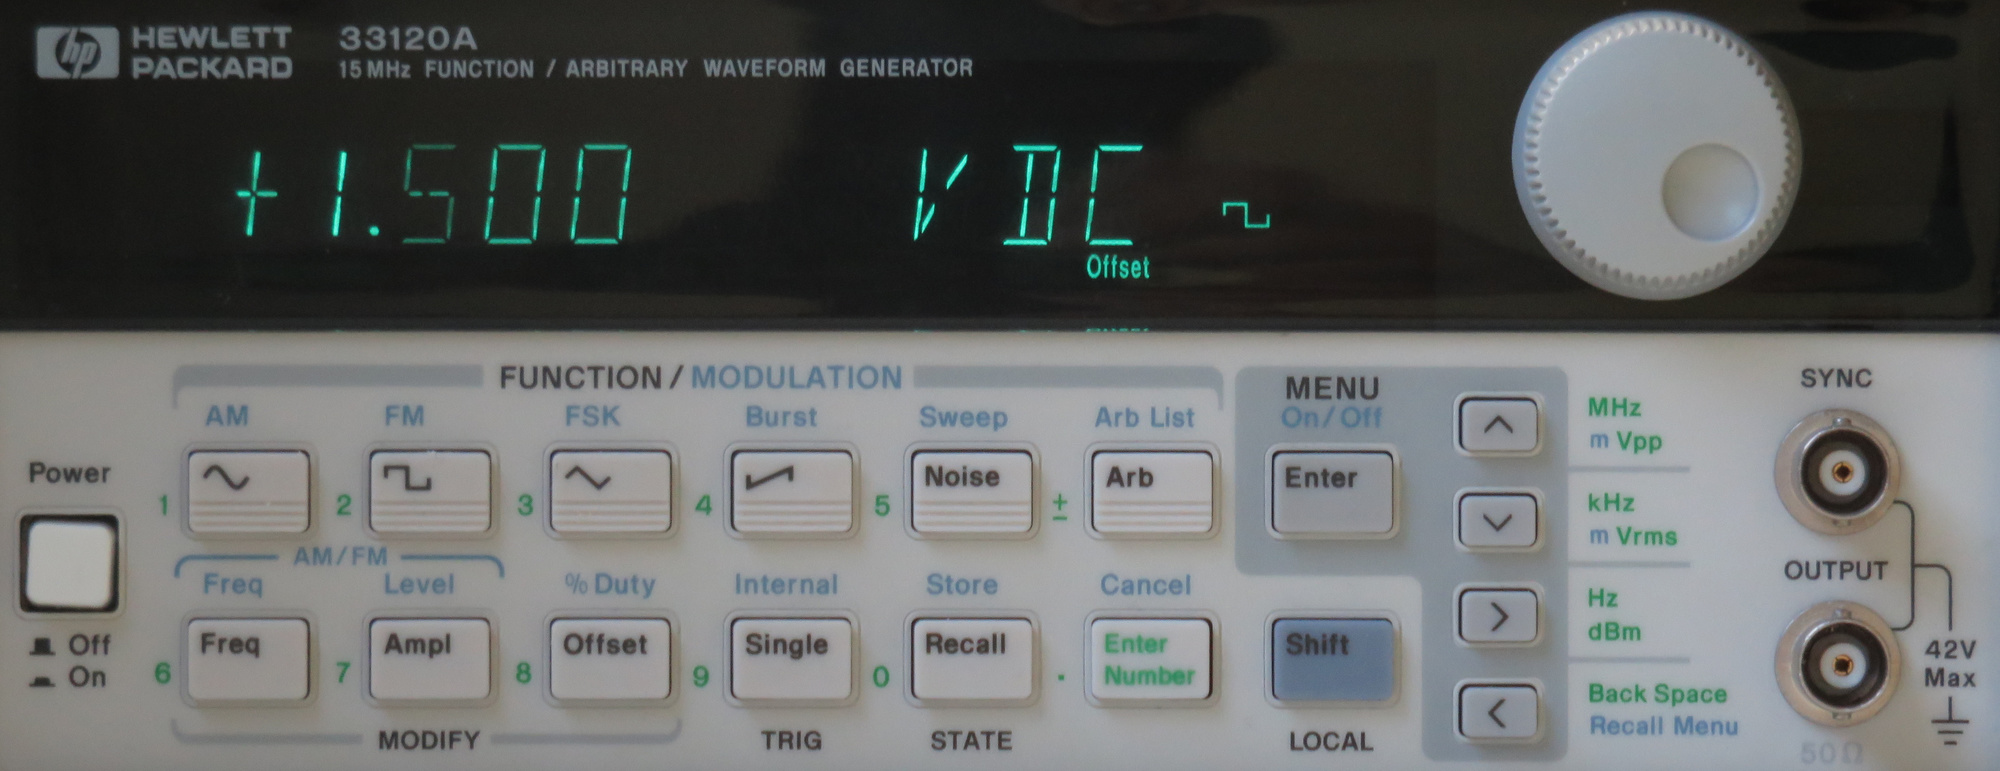
\includegraphics[width=0.67\textwidth]{images/funcGen/funcGen-08.jpg}
    \caption{Offset voltage configuration}
    \label{fig:HPwave:offset}
\end{figure}

\begin{figure}
    \centering
    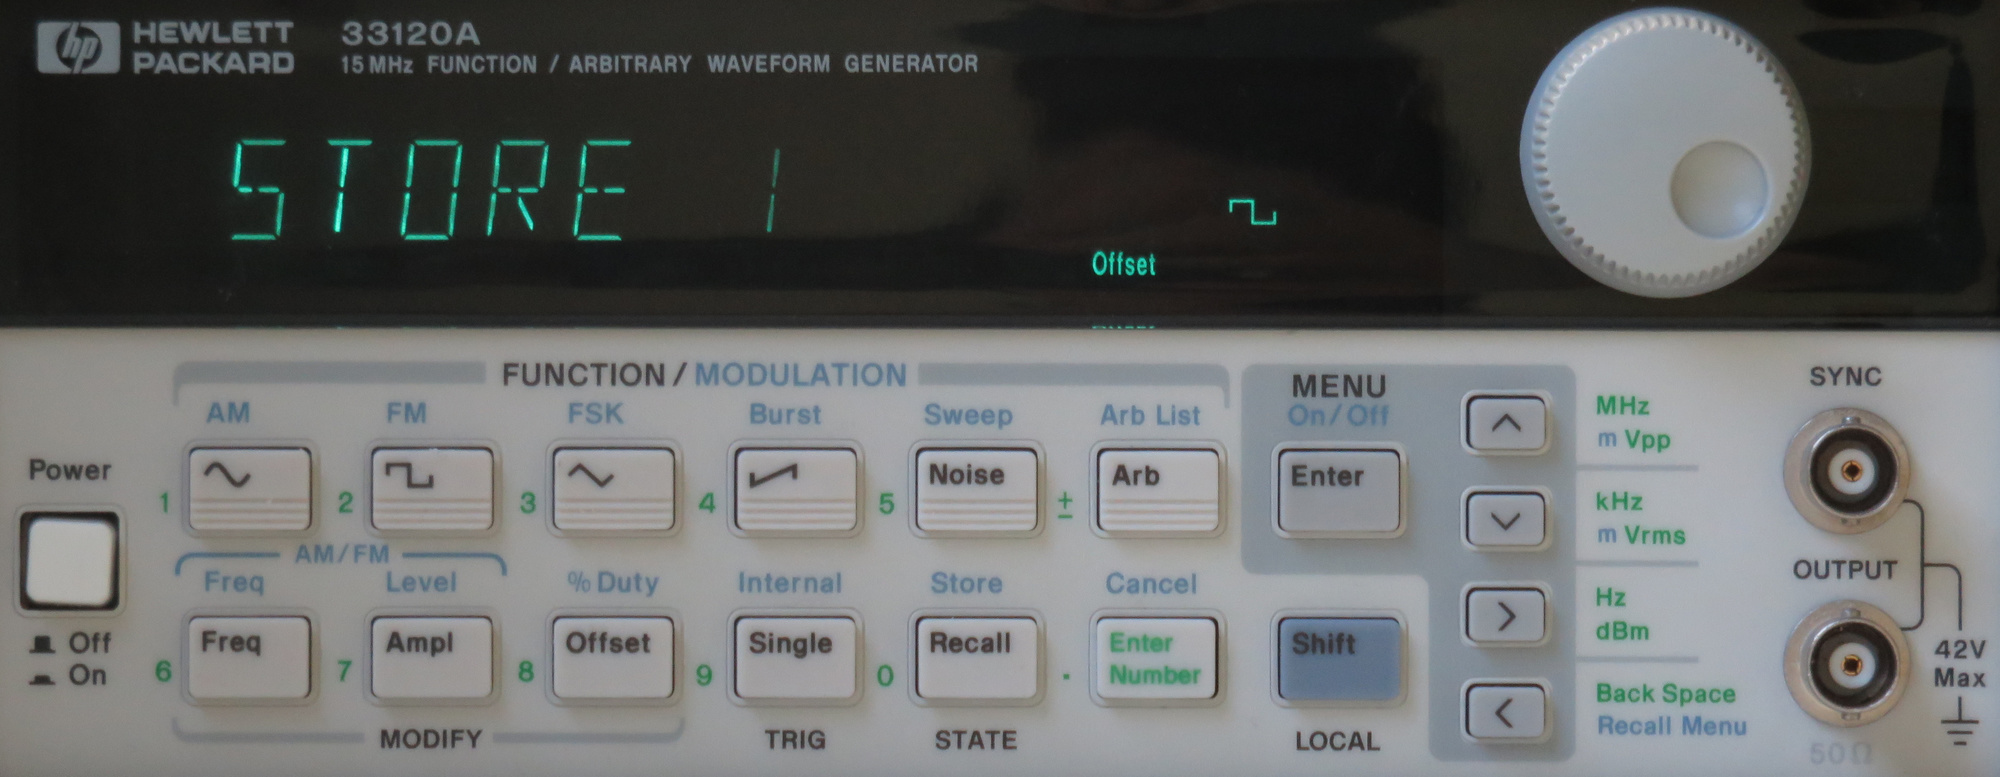
\includegraphics[width=0.67\textwidth]{images/funcGen/funcGen-09.jpg}
    \caption{Storing the configuration in slot 1}
    \label{fig:HPwave:store}
\end{figure}


% ---------------------------------------------------------------------------- %
\clearpage
\subsection{Restoring Configuration}
\label{subsec:HPwave:restoringConfig}
% ---------------------------------------------------------------------------- %

For restoring from a saved configuration, press \emph{RECALL}, select the slot
to be  restored (slot 1  in \fref{fig:HPwave:recall}) and confirm  by pressing
\emph{ENTER}.  The device should now be set to the saved configuration again.

%\begin{figure}
%    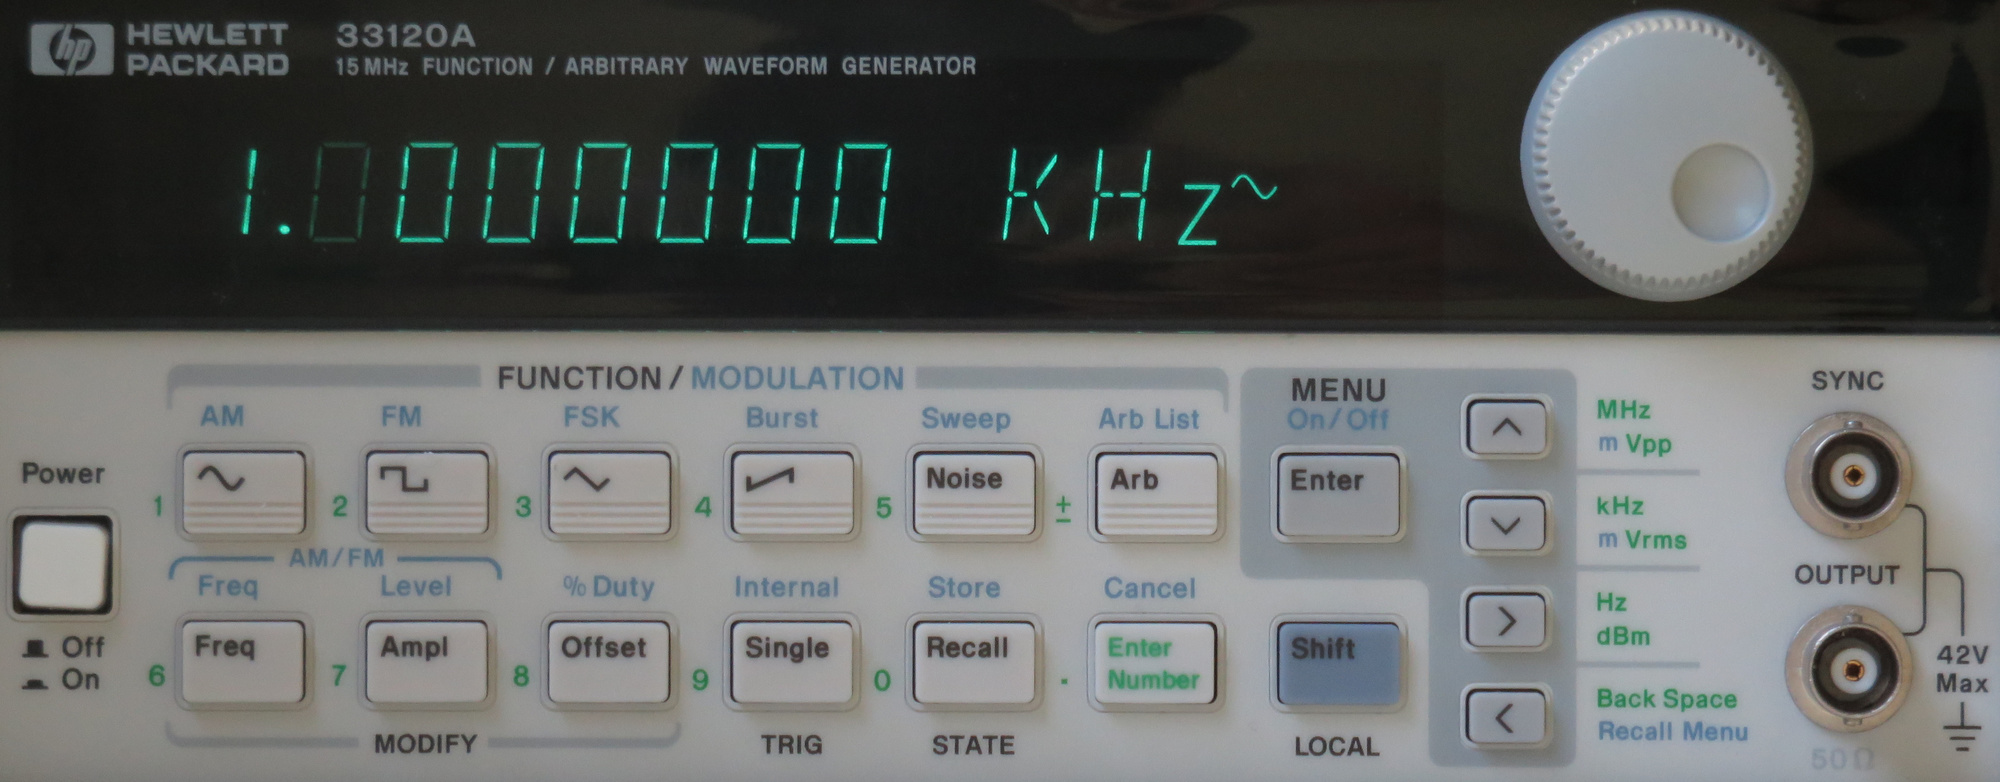
\includegraphics[width=0.67\textwidth]{images/funcGen/funcGen-10.jpg}
%    \caption{Initial screen after power-on}
%    \label{fig:HPwave:poweron}
%\end{figure}

\begin{figure}
    \centering
    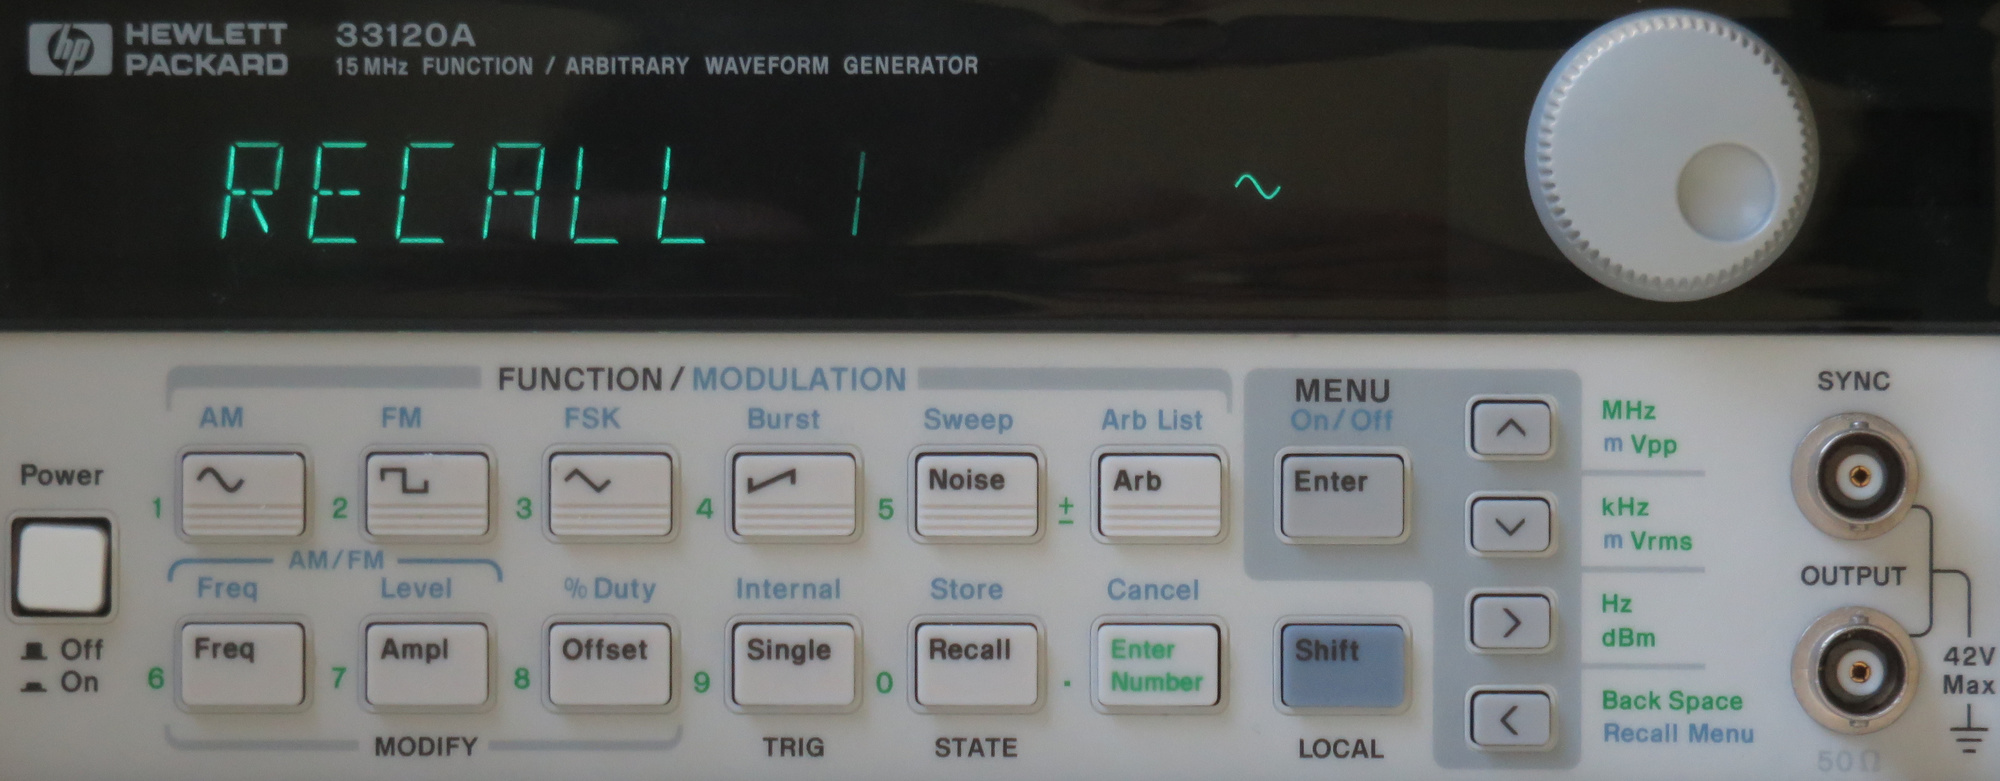
\includegraphics[width=0.67\textwidth]{images/funcGen/funcGen-11.jpg}
    \caption{Initial screen after power-on}
    \label{fig:HPwave:recall}
\end{figure}

%\begin{figure}
    \centering
%    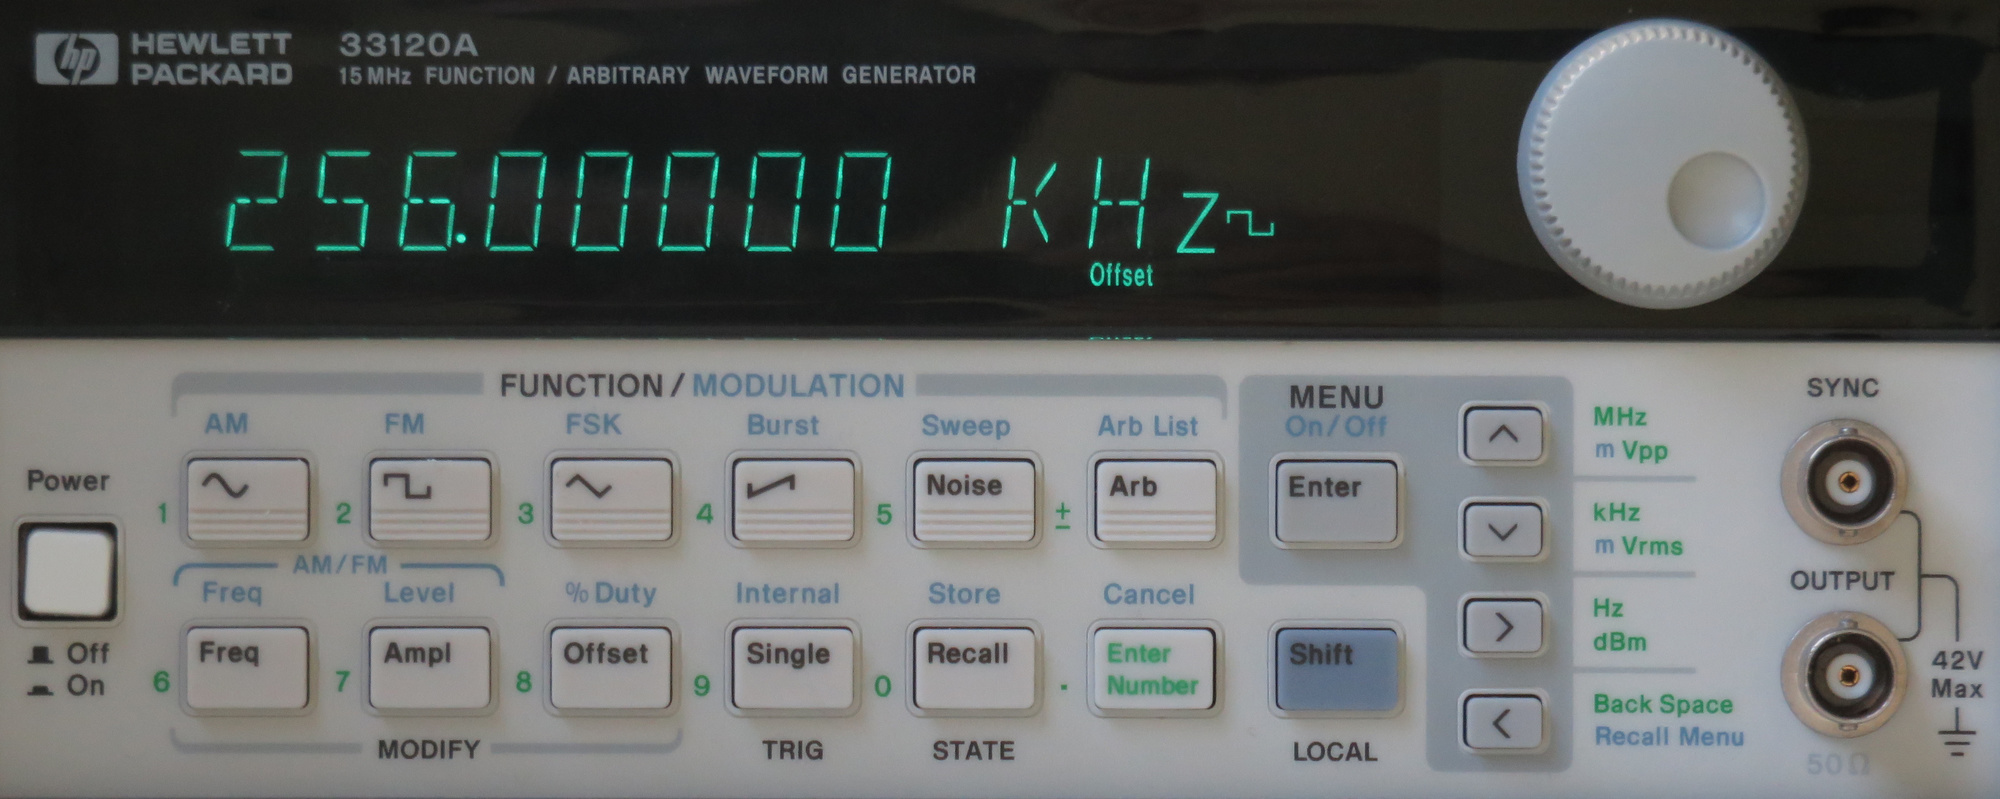
\includegraphics[width=0.67\textwidth]{images/funcGen/funcGen-12.jpg}
%    \caption{Initial screen after power-on}
%    \label{fig:HPwave:poweron}
%\end{figure}

% --------------------------------------------------------------------------- %
\chapter{Scripts}
\label{app:chap:scripts}
% --------------------------------------------------------------------------- %
\todo[inline]{Give locations in repository}
\todo[inline]{shorten/format scripts more sensibly}

This   section   contains   the   various  scripts   which   were   used   for
remote-controlling equipment and for processing data.

% --------------------------------------------------------------------------- %
\section{Waveform Generator Remote Control}
\label{sec:app:33120A}
% --------------------------------------------------------------------------- %
\inputminted{python}{code/33120A.py}

% --------------------------------------------------------------------------- %
\section{Bit Stream Acquisition Program}
\label{sec:app:bitstream:acquisition}
% --------------------------------------------------------------------------- %

\todo[inline]{Insert \raspi~scripts and stuff}

% --------------------------------------------------------------------------- %
\section{Bit Stream Acquisition Control Script}
\label{sec:app:bitstream:control}
% --------------------------------------------------------------------------- %

This script runs on a PC and
\begin{itemize}\tightlist
    \item
    sets the sampling frequency,
    \item
    sets the input voltage,
    \item
    starts the bit stream acquisition on the \raspi,
    \item
    and downloads the data back to the PC.
\end{itemize}

The measurement data can then be processed with the filter script from section
\todo[inline]{insert a section with the new bitstream plotting script}.

\inputminted{shell}{code/measure--sigdel--1-3-11.sh}

% --------------------------------------------------------------------------- %
\section{Bit Stream Evaluation Script}
\label{sec:app:bitstream:filter}
% --------------------------------------------------------------------------- %
\todo[inline]{bitstream python plotting script}

% --------------------------------------------------------------------------- %
\section{WaveRunner 6100A Configuration}
\label{sec:app:waveRunner:acquire}
% --------------------------------------------------------------------------- %
\inputminted{python}{code/configWaveRunner.py}

% --------------------------------------------------------------------------- %
\section{WaveRunner 6100A Data Acquisition}
\label{sec:app:waveRunner:acquire}
% --------------------------------------------------------------------------- %
\inputminted{python}{code/acquireWaveRunnerData.py}

% --------------------------------------------------------------------------- %
\section{Master Control Script for Analog Measurements}
\label{sec:app:masterScript}
% --------------------------------------------------------------------------- %
\inputminted{shell}{code/measure--gain01--1-1-3-11.sh}

%\include{appendices/costs}
%\include{appendices/datentrager}

% -------------------------------------------------------- %
% Page  numbering continues,  but chapter  numbers are  no %
% longer  displayed. See  memoir  documentation  for  more %
% information.                                             %
% -------------------------------------------------------- %
%\backmatter

\end{document}
